\documentclass{ieeeaccess}
\usepackage{cite}
\usepackage{amsmath,amssymb,amsfonts}
\usepackage{algorithm}
\usepackage{algorithmic}
\usepackage{graphicx}
\usepackage{textcomp}
\usepackage{subfigure}
\usepackage{epstopdf}
\usepackage{url}

\graphicspath{{../}}
\epstopdfsetup{
    program@epstopdf=epstopdf
}

\newcommand{\brho}{\boldsymbol{\rho}}
\newcommand{\brhop}{\boldsymbol{\rho^\prime}}
\newcommand{\Es}{\mathbf{E^S}}
\newcommand{\GS}{\mathbf{G^S}}
\newcommand{\X}{\boldsymbol{\chi}}
\newcommand{\E}{\mathbf{E}}
\newcommand{\Xo}{\boldsymbol{\bar{\chi}_o}}
\newcommand{\Xr}{\boldsymbol{\bar{\chi}_r}}


\usepackage{bm}
\makeatletter
\AtBeginDocument{\DeclareMathVersion{bold}
\SetSymbolFont{operators}{bold}{T1}{times}{b}{n}
\SetSymbolFont{NewLetters}{bold}{T1}{times}{b}{it}
\SetMathAlphabet{\mathrm}{bold}{T1}{times}{b}{n}
\SetMathAlphabet{\mathit}{bold}{T1}{times}{b}{it}
\SetMathAlphabet{\mathbf}{bold}{T1}{times}{b}{n}
\SetMathAlphabet{\mathtt}{bold}{OT1}{pcr}{b}{n}
\SetSymbolFont{symbols}{bold}{OMS}{cmsy}{b}{n}
\renewcommand\boldmath{\@nomath\boldmath\mathversion{bold}}}
\makeatother

\def\BibTeX{{\rm B\kern-.05em{\sc i\kern-.025em b}\kern-.08em
    T\kern-.1667em\lower.7ex\hbox{E}\kern-.125emX}}

%Your document starts from here ___________________________________________________
\begin{document}
\history{}
\doi{}

\title{Performance Indicators for Shape and Position Assessment in Electromagnetic Inverse Scattering}
\author{\uppercase{Andr\'e Costa Batista}\authorrefmark{1,2} and
\uppercase{Ricardo Adriano}\authorrefmark{2}}

\address[1]{Operations Research and Complex Systems Laboratory (ORCS Lab), Belo Horizonte, MG 31270-901,, Brazil.}
\address[2]{Department of Electrical Engineering, Universidade Federal de Minas Gerais, Belo Horizonte, MG 31270-901, Brazil.}
\tfootnote{This work was supported in part by the Brazilian agency CAPES (Coordination for the Improvement of Higher Education Personnel) under Grant 88887.463864/2019-00, the scholarship FAPEMIG-CNPQ (process APQ-06716-24), and CNPq (The National Council for Scientific and Technological Development).The Article Processing Charge for the publication of this research was funded by the Coordination for the Improvement of Higher Education Personnel - CAPES (ROR identifier: 00x0ma614). For open access purposes, the authors have applied the Creative Commons CC BY license to any accepted version of the article.}

\markboth
{Batista \& Adriano: Performance Indicators for Shape and Position Assessment in Electromagnetic Inverse Scattering}
{Batista \& Adriano: Performance Indicators for Shape and Position Assessment in Electromagnetic Inverse Scattering}

\corresp{Corresponding author: André Costa Batista (e-mail: andre-costa@ufmg.br).}


\begin{abstract}
Microwave imaging is a low-cost, non-invasive technique for detecting and characterizing objects in inaccessible media through electromagnetic field measurements. The evaluation of algorithms that solve the related electromagnetic inverse scattering problem typically relies on metrics such as Mean Square Error (MSE) or Structural Similarity (SSIM), which primarily assess contrast estimation accuracy but provide limited insight into the recovery of object geometry and position. To address this limitation, this paper introduces two novel performance indicators specifically designed to evaluate electromagnetic inverse scattering algorithms: a shape error indicator that quantifies geometric reconstruction accuracy, and a position error indicator that measures object localization precision. The proposed indicators are applicable to both qualitative and quantitative methods, even when they are combined in an experiment. Comprehensive experimental validation is conducted using traditional algorithms: Linear Sampling Method (LSM), Orthogonality Sampling Method (OSM), Born Iterative Method (BIM), Contrast Source Iterative Method (CSI), Subspace Optimization Method (SOM), and Circle Approximation (CA). Three distinct experimental frameworks are employed: shape recovery studies, position detection studies, and a realistic breast phantom study demonstrating their applicability. Supported by robust statistical analysis, the experiments revealed that: (a) in scenarios with a single scatterer and low Degree of Nonlinearity, BIM achieves the best average performance in object geometry recovery; (b) in scenarios with a single small-sized, high-contrast scatterer, SOM and OSM achieve the best average performance in target localization; and (c) the proposed indicators are less sensitive to contrast estimation errors compared to traditional metrics like MSE and SSIM and to shape reconstruction errors when location detection is considered. These indicators provide useful tools for algorithm development, benchmarking studies, and performance assessment in electromagnetic inverse scattering applications.
\end{abstract}

\begin{keywords}
Algorithm evaluation, electromagnetic inverse scattering, microwave imaging, performance indicators.
\end{keywords}

\titlepgskip=-21pt

\maketitle

\section{Introduction}\label{sec:introduction}

    \PARstart{M}{icrowave} Imaging is an important technique for the detection and characterization of objects in inaccessible media \cite{pastorino2010microwave}. This low-cost technique uses low-power electromagnetic waves to obtain information about the internal structure of materials in a non-invasive manner \cite{godinho2025evaluation}. The applications of this method are diverse, including medical diagnostics \cite{mojabi2025microwave}, structural inspection \cite{fedeli2025mild}, through-wall imaging \cite{fedeli2020through}, remote sensing \cite{salucci2017multifrequency}, among others.

    This technique is based on solving the inverse electromagnetic scattering problem \cite{chen2018computational}. Specifically, electromagnetic field measurements collected outside the Domain of Interest (DOI) are used to recover the properties of the internal medium. This problem is inherently ill-posed, meaning that small variations in measurements can lead to large variations in the solution \cite{colton2019inverse}. Furthermore, the problem is both nonlinear and non-convex due to multiple scattering effects \cite{chen2018computational}. The problem can be formulated in either two or three dimensions, with two-dimensional formulations being more commonly used for algorithm development due to their computational simplicity and efficiency.

    A wide range of algorithms exists for solving the inverse electromagnetic scattering problem. These algorithms can be broadly classified into two main categories: qualitative methods \cite{pastorino2010ch5}, which reconstruct images without estimating the electrical properties of the medium, and quantitative methods \cite{pastorino2010ch7}, which estimate these properties. 

    Among qualitative methods, notable examples include the Linear Sampling Method (LSM) \cite{chen2017lsm} and the Orthogonality Sampling Method (OSM) \cite{harris2020orthogonality}. Among quantitative methods, prominent approaches include the Born Iterative Method (BIM) \cite{wang1989iterative}, Contrast Source Inversion (CSI) \cite{berg1997contrast}, the Distorted Born Inversion Method (DBIM) \cite{chew1990reconstruction}, and the Subspace Optimization Method (SOM) \cite{chen2010subspace}.

    Specialized algorithms have been developed to address specific problem characteristics. These include the DORT method (Decomposition of the Time-Reversal Operator) \cite{chen2018computational} for electromagnetic signal time reversal, Multiple Signal Classification (MUSIC) \cite{zhong2007music} for small scatterers, and Compressive Sensing \cite{massa2015compressive} for phaseless field data. For weak scatterer problems, effective approaches include First-Order Born Approximation, Backpropagation, and Rytov approximation \cite{chen2018computational}. 

    Additional relevant techniques include Virtual Experiments \cite{isernia2024some,bevacqua2021simple}, which recombine scattered field data to explore conditions that alleviate nonlinearity, and efficient equation reformulations \cite{isernia2024some,bevacqua2021effective} that share the same objective of reducing nonlinearity.

    Recently, machine learning-based algorithms have emerged as promising solutions \cite{chen2020review}. Among these approaches, data-driven methods such as the Direct Inversion Scheme \cite{yao2020enhanced,wei2019solving} enable direct inference of scatterer physical parameters from measured fields, minimizing preprocessing requirements. However, these methods often demand extensive training datasets and exhibit significant limitations in generalization, reliability, and interpretability. 

    To address these deficiencies, physics-driven methods have been proposed that incorporate physical laws and information to guide the reconstruction process \cite{wei2019physics,wang2023push,hu2023more,liu2025exploring}. Another approach involves constructing surrogate models for recovering scatterer position, geometry, and contrast through optimization problems \cite{salucci2022learned,zardi2025physics}. Despite overcoming some limitations of purely data-driven approaches, their effectiveness may depend on system parameters such as the Green's function, whose determination in complex or inhomogeneous media represents a significant challenge.

    In most of these studies, the proposed algorithms are tested and evaluated using metrics such as the Mean Square Error (MSE) of pixel-by-pixel contrast estimation or similar approaches \cite{yin2023subspace,zhang2023iterative,salucci2022learned,wang2023push,liu2022som,bevacqua2021simple,bevacqua2021effective}. This type of approach directly considers the precision of contrast estimation and can indirectly provide perspective on how well the reconstruction of object position and geometry might be, since errors in geometry and positioning can affect this metric. However, a highly accurate geometry with poor contrast estimation can result in considerable error in this type of metric, for example. Therefore, aspects of comparing performance regarding how well object geometry and position are recovered are not adequately addressed by this type of metric. Furthermore, the MSE metric is not suitable for evaluating qualitative algorithms, since these do not estimate the medium's contrast.

    It is also worth highlighting the Structural Similarity (SSIM) metric \cite{wang2004image} for quantifying reconstruction visual quality, which is designed to compute the mismatch between reconstructed contrast results and corresponding ground truths, both at the pixel-wise level and perceptual level \cite{wang2023push,liu2025exploring}. Instead of performing a pixel-by-pixel comparison, this metric considers aspects of luminance, contrast (in the sense of the difference among the pixels values), and structure of any given image. Therefore, while it provides a deeper quantification of overall reconstruction quality, it does not directly measure isolated aspects such as geometry and position. In fact, errors in the dielectric properties estimation can affect this metric, even when the geometry and position are accurately recovered.

    Specifically for breast imaging, a set of metrics has been proposed in the literature that considers not only the precision in estimating electrical properties, but also the accuracy of the reconstructed tissue geometry \cite{kurrant2021evaluating}. Each geometry (original and reconstructed) is converted into vectors, and the metric is calculated using a formula that performs the dot product and norm of these vectors. To the best of the authors' knowledge, this is the only metric that can independently consider the geometry aspect of the scatterer, even though it is designed specifically for breast imaging.

    The objective of this work is to provide additional metrics to assist in evaluating algorithm performance. With a broader range of indicators, it becomes possible to obtain a more comprehensive understanding of algorithm capabilities across different scenarios. Therefore, our contribution is based on proposing two novel indicators for evaluating algorithm performance in recovering scatterer geometry and position. The first indicator quantifies shape error, while the second quantifies position error. 

    The originality of this work lies in the fact that these indicators can measure these two relevant aspects of electromagnetic inverse scattering algorithm performance in a more isolated manner than the existing metrics. Furthermore, these indicators are designed to be applicable to any algorithm that reconstructs images, regardless of whether it estimates contrast or not.

    The remainder of this paper is organized as follows. Section \ref{sec:problemstatement} presents the problem statement and the mathematical formulation of the electromagnetic inverse scattering problem. Section \ref{sec:indicators} introduces the proposed indicators for evaluating algorithm performance. Section \ref{sec:results} presents numerical results demonstrating the effectiveness of the proposed indicators. Finally, Section \ref{sec:conclusion} concludes the paper and discusses future work.

\section{Problem Statement}\label{sec:problemstatement}
    
    Let $D \in \mathbb{R}^2$ denote the DOI embedded within a homogeneous, isotropic, nonmagnetic ($\mu = \mu_0 = 4\pi \times 10^{-7}$ H/m), and lossless ($\sigma = \sigma_0 = 0$ S/m) background medium with permittivity $\epsilon_b = \epsilon_{rb}\epsilon_0$, where $\epsilon_0 \approx 8.85 \times 10^{-12}$ F/m. We consider a 2D Transverse Magnetic (TMz) polarization where the DOI is illuminated by incident plane waves and assume the time convention $e^{j\omega t}$. All scatterers are located within the DOI, and the scattered field $E^s_z$ at point $\brho \in S$ outside $D$ is evaluated according to the following integral equation \cite{harrington2001time}:
    \begin{equation}
        E^s_z (\brho) = -\frac{k_b^2}{4} \int_D H_0^{(2)}(k_b|\brho-\brhop|)\chi(\brhop)E_z(\brhop) dS^\prime
    \end{equation}
    
    \noindent where $k_b = \omega\sqrt{\epsilon_b\mu_0} = 2\pi/\lambda_b$ is the background wave number, $\lambda_b$ is the wavelength of the incident wave, $H_0^{(2)}$ is the zero-order Hankel function of the second kind, $E_z$ is the total electric field in the DOI, and $\chi$ is the contrast function given by
    \begin{equation}
        \chi(\brho) = \frac{\epsilon_r(\brho)}{\epsilon_{rb}} - 1 - j\frac{\sigma(\brho)}{\omega\epsilon_b},
    \end{equation}
    
    \noindent which maps the relative permittivity $\epsilon_r(\brho)$ and conductivity $\sigma(\brho)$ distributions within $D$. It should be noted that the term $(-jk_b^2/4) H_0^{(2)}(k_b|\brho-\brhop|)$ corresponds to the Green's function in free space.
    
    In electromagnetic inverse scattering problems, we aim to recover the contrast function $\chi$ using a set of $N_M$ measurements of the scattered field collected for each of the $N_S$ sources. Additionally, $E_z$ is also unknown in $D$ and must be solved. For our formulation, the $N_S$ sources correspond to $N_S$ incidence angles of the plane wave, and the $N_M$ measurements are taken at $N_M$ points in $S$, arranged in a circular, equidistant array situated far from the center of the DOI by a radius $R_O$. By discretizing the DOI into $N_X \times N_Y = N$ pixels, the inverse problem is solved numerically according to the following equation:
    \begin{equation}
        E^s_{ms} = - \sum\limits_{n=1}^{N} G^S_{mn}\chi_{n}E_{ns} \label{eq:numerical}
    \end{equation}
    
    \noindent where $G^S$ is given according to the Richmond discretization \cite{richmond1965scattering, pastorino2010ch3}. Equation \eqref{eq:numerical} can also be expressed in matrix form:
    \begin{equation}
        \Es = \GS\X\E
    \end{equation}
    
    \noindent where $\Es$ is the $N_M \times N_S$ scattered field matrix, $\GS$ is the $N_M \times N$ Green's function matrix, $\X$ is the $N \times N$ contrast diagonal matrix, and $\E$ is the $N \times N_S$ total electric field matrix.
    
    It is important to highlight that, although assumptions are made regarding the scattered field domain and the incident field, the proposed indicators do not depend on these assumptions. They can be applied in any scenario where these entities are defined, and the assumptions in this paper serve only to clearly establish the context in which the indicators are tested.

\section{Indicators}\label{sec:indicators}

    Once the result of the contrast function reconstruction is obtained by a given algorithm, the error in recovering the shape and location of the objects can be measured by comparing it with the original images. This means that the application of these metrics is relevant in studies where the exact response is known. Although in many real-world scenarios the imaged scatterer is unknown, applying these metrics to known cases can be valuable for comparing the performance of different algorithms and for estimating a confidence interval for the average performance of an algorithm in a given configuration. Therefore, these metrics are relevant tools that can contribute to the investigation and evaluation of algorithms for the problem.
    
    For the two indicators that will be explained below, the image of the original contrast function of the problem and the image reconstructed by any algorithm will be denoted by the matrices $\Xo$ and $\Xr$, both of size $N_X \times N_Y$. In other words, the elements of these matrices represent the pixels of the images.

    \subsection{Shape Error}\label{sec:indicators:shapeerror}

        The contrast function has complex values when the medium or the scatterers have losses. Therefore, the first step is to account for the possibility that the elements of the matrices $\Xo$ and $\Xr$ have real and imaginary parts. The simplest approach is to use the magnitude of the complex variables as the value of each pixel. This choice does not eliminate the possibility that objects with different contrasts might have the same magnitude. However, in cases involving only lossless materials, this approach is not problematic because the contrast is purely real. Since the primary objective is to verify the shape of the scatterers, the critical aspect is distinguishing between the background medium and the scatterer, with the background medium having zero contrast. Thus, this approach to simplifying the methodology for measuring shape error should not have significant consequences in performance verification scenarios for the algorithm.

        The contrast function reconstructed by many algorithms -- such as BIM, DBIM, CSI, SOM, among others -- is commonly a discretized approximation of a continuous surface. Therefore, even if the original image contains only objects with well-defined boundaries and homogeneous contrast, the image of these objects obtained by the algorithms will frequently have smooth edges, i.e., the contrast value gradually varies between the background medium and the object's value. Consequently, identifying a contour in the resulting image is heuristic because it requires selecting a criterion to define the contrast value at which a pixel can be considered as belonging to the object. For simplicity, the threshold $T$ for considering a pixel in the recovered image to be within an object's contour will be defined as half of the total contrast variation in the image, i.e.:
        \begin{equation}
            T = \min(|\Xr|) + \frac{1}{2} \left[\max(|\Xr|)-\min(|\Xr|)\right]
        \end{equation}

        This approach has advantages and disadvantages. If the reconstructed image contains multiple scatterers where one or more has a contrast below this threshold, the methodology will fail to detect the contour of these objects. However, in scenarios with a single scatterer, this approach is simple and effective. Single scatterer scenarios represent the most objective way to test an algorithm's geometry recovery potential, since multiple scatterers can degrade performance due to mutual current induction effects between objects.

        This approach poses no issues for algorithms capable of accurately capturing contours, such as machine learning-based methods. Furthermore, using only values from the reconstructed image (rather than the original image) helps isolate contrast estimation errors and enables metric application to qualitative methods that do not estimate contrast. When the original contrast function involves soft object boundaries, the threshold may also be applied to the original image for consistency.

        Once the thresholding step is applied, the contours of the scatterers can be determined. One of the techniques suitable for this task is the Marching Squares algorithm \cite{lorensen1987marching}. This algorithm efficiently returns a set of points that delineate each contour. It is important to note that hollow objects may have two or more contours. Additionally, if the imaging algorithm fails to detect an object, a discrepancy will arise in the number of contours between the original and reconstructed images.
        
        For these reasons, instead of comparing the geometries through calculations based on the points of each contour, we prefer to perform the comparison based on the number of pixels that were misclassified. Specifically, after identifying which pixels fall within each contour in each image, we can determine which pixels belonged to the scatterers in the original image but were not captured in the reconstructed image (false negatives) and which pixels did not belong to the scatterers in the original image but were classified as such in the reconstructed image (false positives).
        
        A potential question that may arise from this choice is why not directly calculate false positives and false negatives immediately after thresholding. One reason is that original and reconstructed images typically have different resolutions. While the nearest neighbor interpolation method is an alternative for addressing this issue, the chosen approach may be more effective for capturing and preserving object contours, particularly when the resolution of the reconstructed image is significantly lower. This is illustrated in Fig. \ref{fig:contourmotivation}.

        \begin{figure}[!t]
            \centering
            \subfigure[]{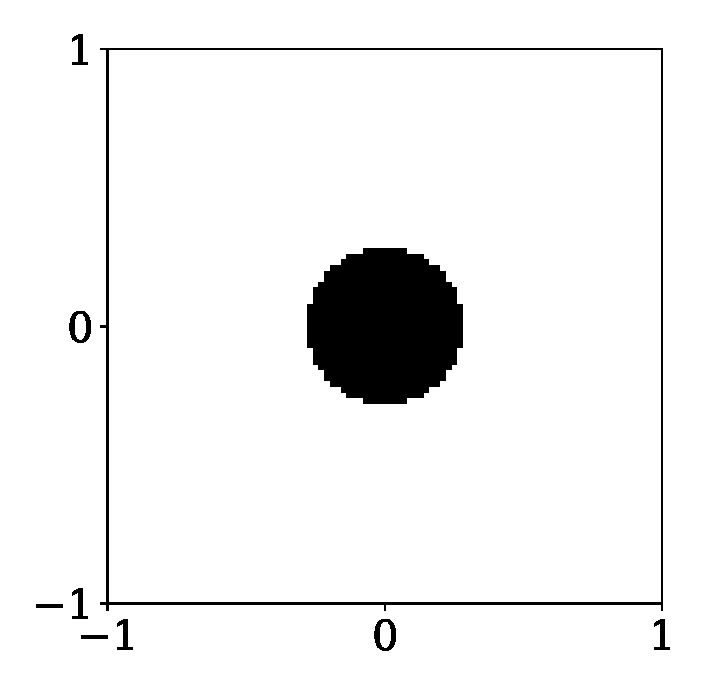
\includegraphics[width=.49\columnwidth]{./figs/batis01}}
            \subfigure[]{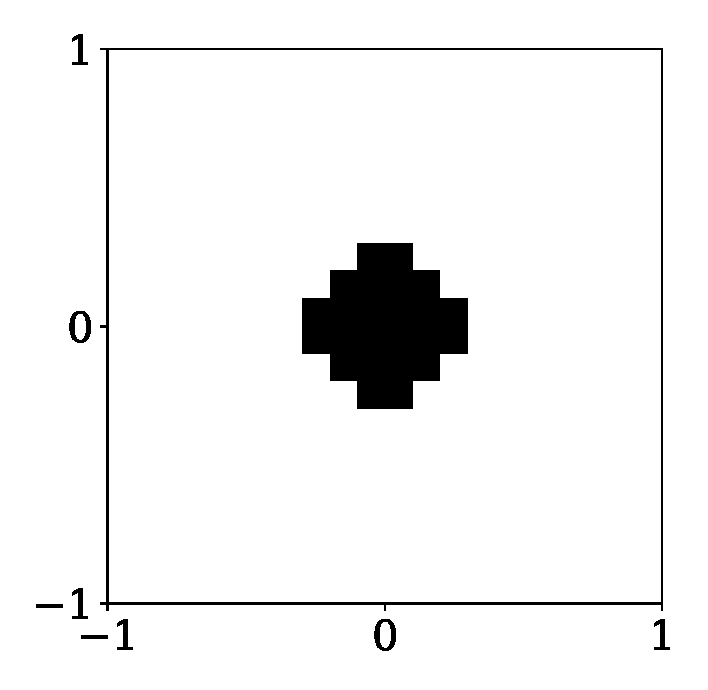
\includegraphics[width=.49\columnwidth]{./figs/batis02}} \\
            \subfigure[]{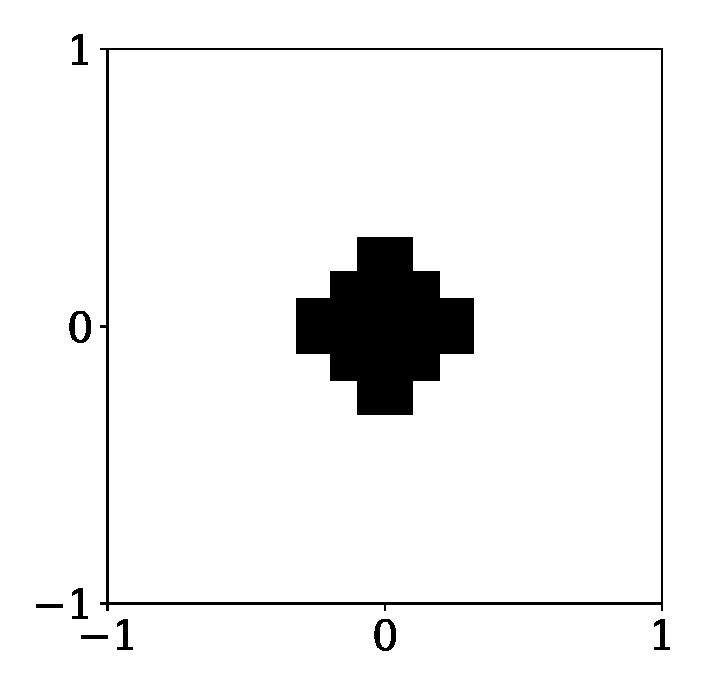
\includegraphics[width=.49\columnwidth]{./figs/batis03}}
            \subfigure[]{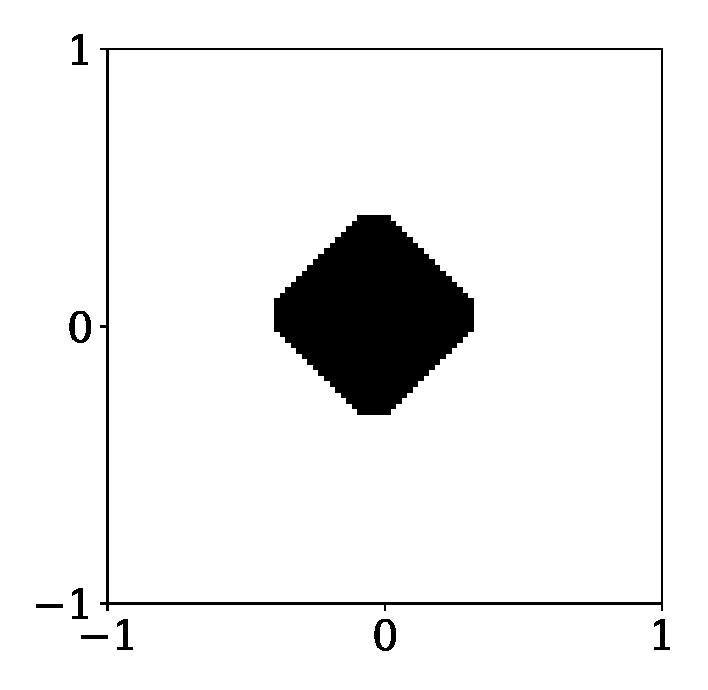
\includegraphics[width=.49\columnwidth]{./figs/batis04}}
            \caption{An example illustrating the differences between nearest neighbor interpolation and the adopted contour detection methodology. (a) Original image of the scatterer (resolution 100x100); (b) Image reconstructed by an imaging algorithm after thresholding (20x20); (c) Image reconstructed to the original resolution using nearest neighbor interpolation; (d) Image reconstructed to the original resolution using contour identification.}
            \label{fig:contourmotivation}
        \end{figure}

        The sum of false negatives and false positives can be easily obtained by applying the XOR operation between the two images. Then, we can compute the shape error as the ratio between the number of incorrectly classified pixels and the total number of pixels that are part of the scatterers in the original image. Additionally, if we consider the shape error in percentage values, we can then define the indicator $\zeta_S$ as
        \begin{equation}
            \zeta_S = \frac{\text{FP} + \text{FN}}{\text{TP}} \times 100\%, \label{eq:shapeerror}
        \end{equation}

        \noindent where $\text{FP}$ and $\text{FN}$ are the numbers of false-positive and false-negative pixels, respectively, and $\text{TP}$ is the total number of pixels that are part of the scatterers in the original image. Therefore, the indicator assumes values greater than or equal to zero. Note that values greater than 100\% are also possible, indicating that the reconstructed image has more incorrectly classified pixels than the total number of pixels that make up the scatterers in the original image. This can occur more frequently when the number of pixels of the scatterer in the original image is small. 

        It is important to note that the minimum value of $\text{TP}$ is constrained to 1, since a value of 0 would imply the absence of scatterers in the original image, which is not presumed in performance evaluation scenarios. This constraint ensures numerical stability in the indicator calculation. When dealing with very small scatterers (few pixels), the shape error indicator may produce large percentage values. However, this behavior is meaningful rather than problematic, as even small absolute errors in shape reconstruction represent significant relative errors for small targets. For instance, if a scatterer occupies only 10 pixels and the reconstruction incorrectly classifies 15 pixels, the resulting 150\% error accurately reflects that the reconstruction has more misclassified pixels than the actual object size, providing relevant information about algorithm performance in challenging scenarios.
        
        For scenarios involving small targets where shape reconstruction is particularly challenging, the position error indicator $\zeta_P$ (described in Section \ref{sec:indicators:positionerror}) provides a complementary and more stable performance measure. Algorithm \ref{alg:compute_zeta_s} summarizes the steps for calculating the shape error indicator.

        \input{algorithms/zetas.tex}

    \subsection{Position Error}\label{sec:indicators:positionerror}

        The methodology for calculating the position detection error shares similarities with that of shape error calculation. As it is done when computing the shape error, the position error calculation also uses the absolute value of the image contrasts and applies the same thresholding operation. The reasons for this approach are the same.

        The key difference lies in the method of position error calculation, which is based on comparing the centroid of pixels classified as objects by the thresholding operation in each image. Specifically, the centroid for each image is determined by averaging the coordinates of the pixels that constitute the objects. This method does not require contour detection, as the coordinate points are within the same boundaries for both images, even when resolutions differ.

        The position error indicator is then defined as the Euclidean distance between the centroids in the two images. It is important to note that these centroids are normalized within a range of 0 to 1, where 0 represents the image's origin and 1 represents its end. By multiplying this distance by 100, the error can be interpreted as a percentage relative to the image size. Thus, the indicator quantifies the error in object localization relative to the image size, allowing its application across test sets with varying domain sizes. Therefore, the position error indicator $\zeta_P$ is defined as:
        \begin{equation}
            \zeta_P = \sqrt{(x_c^R - x_c^O)^2 + (y_c^R-y_c^O)^2} \times 100\%, \label{eq:positionerror}
        \end{equation}

        \noindent where $(x_c^R, y_c^R)$ and $(x_c^O, y_c^O)$ are the centroids of the reconstructed and original images, respectively.

        It should be noted that inaccuracies in the reconstructed geometry of objects can significantly influence the position error calculation. For example, if a star-shaped object with five points is reconstructed with one point distorted, this distortion will affect the object's centroid, thereby impacting the position error. However, this effect is expected, as any criterion for determining an object's position inherently considers the pixels defining it, just as it does for its geometry. Furthermore, the proposed indicator is straightforward and versatile, applicable even in scenarios involving images with multiple objects. The Algorithm \ref{alg:compute_zeta_p} summarizes the steps for calculating the position error indicator.

        \input{algorithms/zetap.tex}

\section{Computational Experiments}\label{sec:results}

    The experiments presented in this article are intended to illustrate the application of the proposed indicators. The design of these experiments focuses on demonstrating the potential utility of these indicators, rather than achieving pioneering results in the field. Nevertheless, the findings from these experiments can still provide a foundation for further research by the scientific community.

    The experiments were conducted using the open-source library EISPY2D \cite{batista2025eispy2d}, specifically developed to design and evaluate algorithms for the inverse electromagnetic scattering problem. Both indicators will be analyzed, with each approach featuring two case studies (one fundamental and the other exploring a particular aspect) as well as a benchmarking study. The case studies aim to assess performance in specific scenarios, while the benchmarking study facilitates broader generalization of the results. Additionally, an experiment considering a breast imaging scenario was conducted to illustrate the applicability of the proposed indicators in a realistic scenario. For both indicators, a comparison against communly used metrics, such as MSE and SSIM, will be presented to highlight the differences in the information provided by each metric.

    For all experiments in Section \ref{sec:results:shape} and \ref{sec:results:position}, the following common parameters were used: background wavelength $\lambda_b = 1$ m, noise level of 5\%, relative permittivity of the background medium $\epsilon_{rb} = 1$, and incident wave amplitude of 1 V/m. 

    Data synthesis was performed using the MoM-CG-FFT algorithm \cite{su1987calculation} with 5000 iterations. The measurement configuration consisted of 80 measurement points ($N_M$) and 80 incidence angles ($N_S$), with measurement points arranged in a circular array at distance $R_O = 4\lambda_b$ from the DOI center. 

    The DOI dimensions were set to $2\lambda_b \times 2\lambda_b$, and all reconstructions were performed using a $40 \times 40$ pixel discretization. All implementations necessary for this work are available in the repository at \url{https://github.com/andre-batista/PISPAEIS} for reproducibility purposes.

    \subsection{Shape Recovering Study}\label{sec:results:shape}

        To evaluate shape error, two case studies were conducted. The first case study involves a single scatterer with homogeneous contrast, while the second case study involves a scatterer with variable contrast. These case studies were selected to demonstrate the application of the proposed indicator in typical scenarios encountered in electromagnetic scattering problems. Additionally, a benchmarking study was performed to assess the average performance of algorithms in more general situations. Finally, the proposed shape error indicator was compared with the MSE and SSIM metrics to highlight the differences in the information provided by each metric.

        \subsubsection{Single scatterer}\label{sec:results:shape:star}

            The first case study was designed to evaluate the applicability of the proposed indicator in a straightforward scenario where various algorithms could be applied. This case study features a scatterer shaped like a five-pointed star, centrally positioned within the image. This choice was made to select a geometry that, while symmetric and well-defined, has more vertices compared to more common shapes such as squares or triangles. The contrast was set to 0.25, and the radius from the center of the scatterer to the farthest vertices was set to 0.9$\lambda_b$. Under these conditions, the Degree of Nonlinearity (DNL) for the test is 0.12, which is significantly lower than the threshold beyond which the Born Approximation becomes inapplicable, i.e., 1 \cite{bucci2001degree}. The scattered field was synthesized using a discretization of 120$\times$120 pixels for the original image.

            For this experiment, the following algorithms were considered: LSM, OSM, BIM, CSI, and SOM. Their parameters were chosen after empirical tests that aimed to achieve their best performance. The configurations for each algorithm are as follows:
            \begin{itemize}
                \item Linear Sampling Method (LSM):
                \begin{itemize}
                    \item Threshold: 0.7;
                    \item Regularization Method: Conjugate Gradient with 300 iterations.
                \end{itemize}
                \item Orthogonality Sampling Method (OSM):
                \begin{itemize}
                    \item Threshold: 0.35;
                \end{itemize}
                \item Born Iterative Method (BIM):
                \begin{itemize}
                    \item Regularization Method: Conjugate Gradient with 300 iterations.
                    \item Stopping Criterion: 30 iterations.
                \end{itemize}
                \item Contrast Source Inversion (CSI):
                \begin{itemize}
                    \item Stopping Criterion: 300 iterations.
                \end{itemize}
                \item Subspace Optimization Method (SOM):
                \begin{itemize}
                    \item Stopping Criterion: 30 iterations.
                    \item Eigenvalue Cutoff Index: 5.
                \end{itemize}
            \end{itemize}

            The images reconstructed by each algorithm are shown in Fig. \ref{fig:shape:single:recons}. For the qualitative methods, OSM exhibited contrast variation within the object, which is consistent with the inherent characteristics of the method. Additionally, OSM recovered a larger area with more defined vertices compared to LSM. Regarding the quantitative methods, CSI demonstrated the lowest performance in recovering the object's contrast value close to the ground truth. Moreover, the quantitative methods produced more accurate contours than their qualitative counterparts.

            \begin{figure*}[!htb]
                \centering
                \subfigure[Ground-Truth]{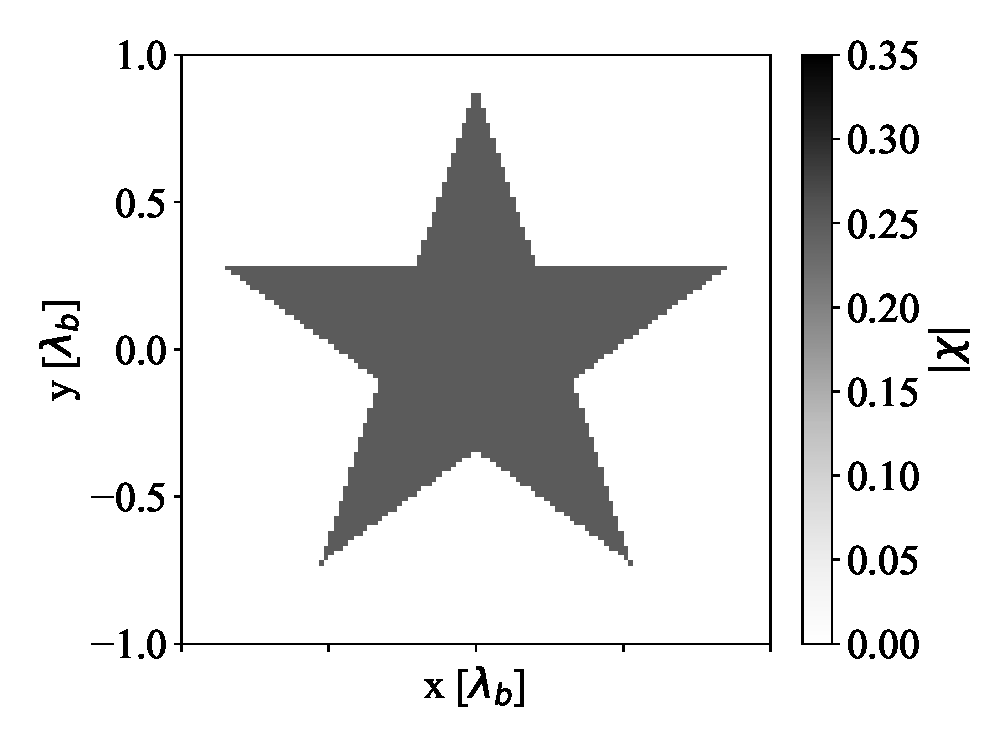
\includegraphics[width=0.3\textwidth]{./experiments/shape/star/figs/0.eps}}
                \subfigure[LSM]{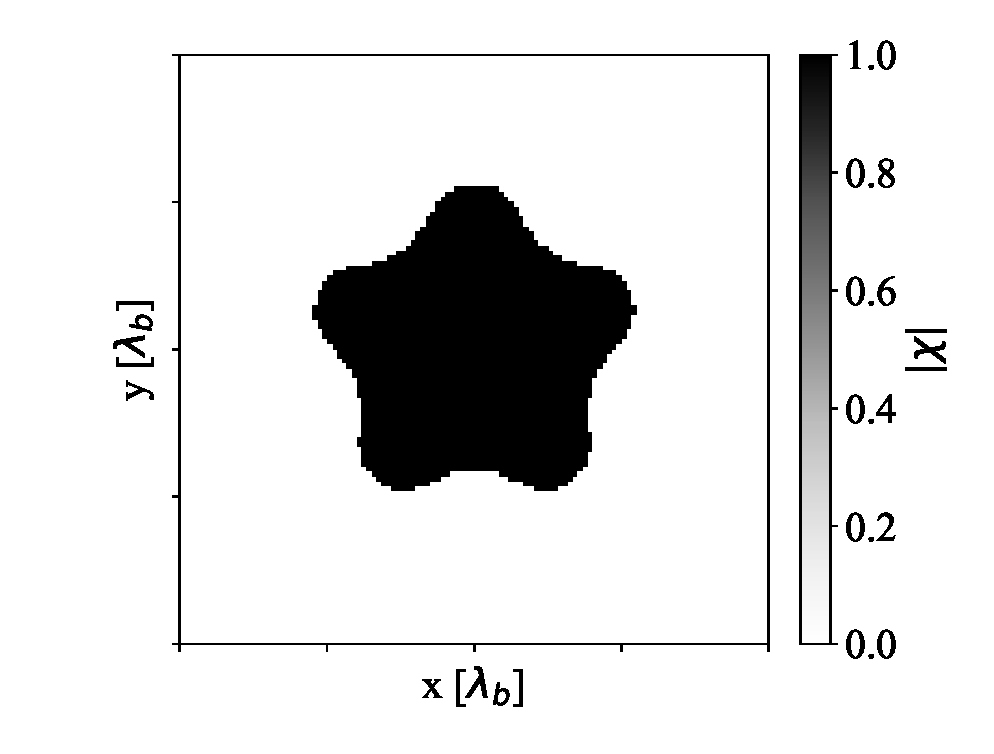
\includegraphics[width=0.3\textwidth]{./experiments/shape/star/figs/1.eps}}
                \subfigure[OSM]{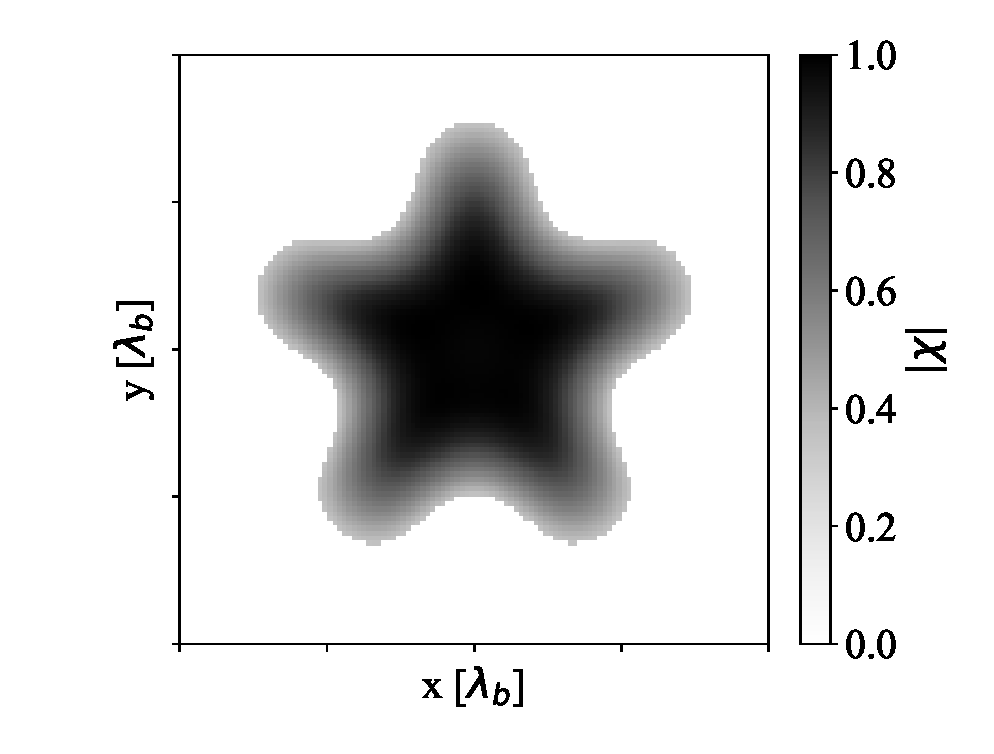
\includegraphics[width=0.3\textwidth]{./experiments/shape/star/figs/2.eps}} \\
                \subfigure[BIM]{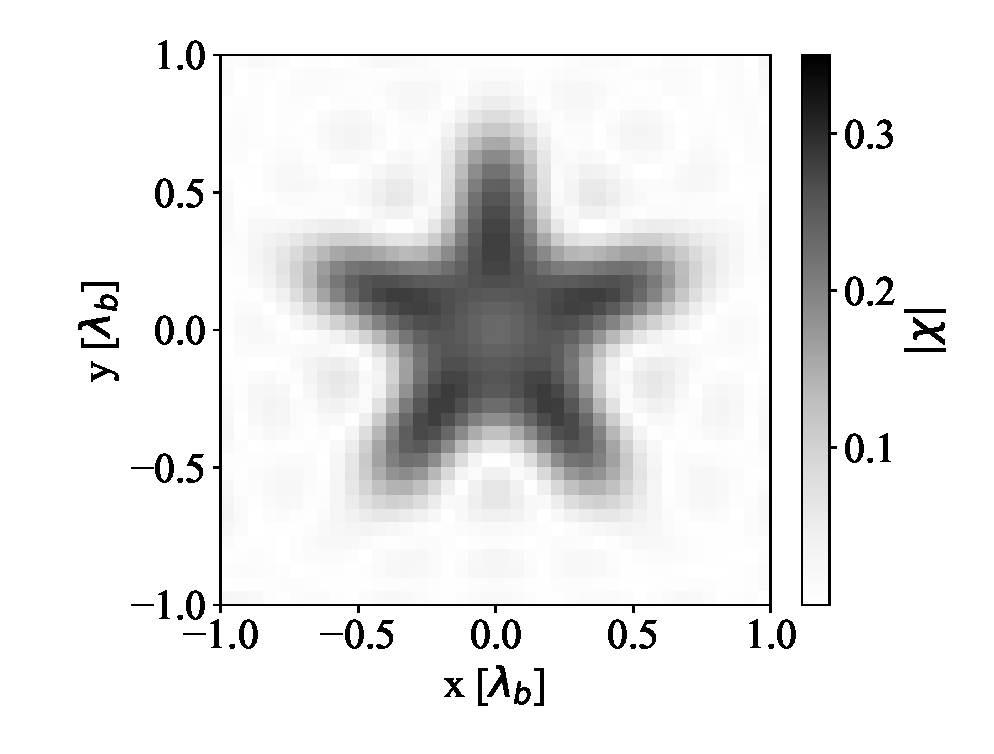
\includegraphics[width=0.3\textwidth]{./experiments/shape/star/figs/3.eps}}
                \subfigure[CSI]{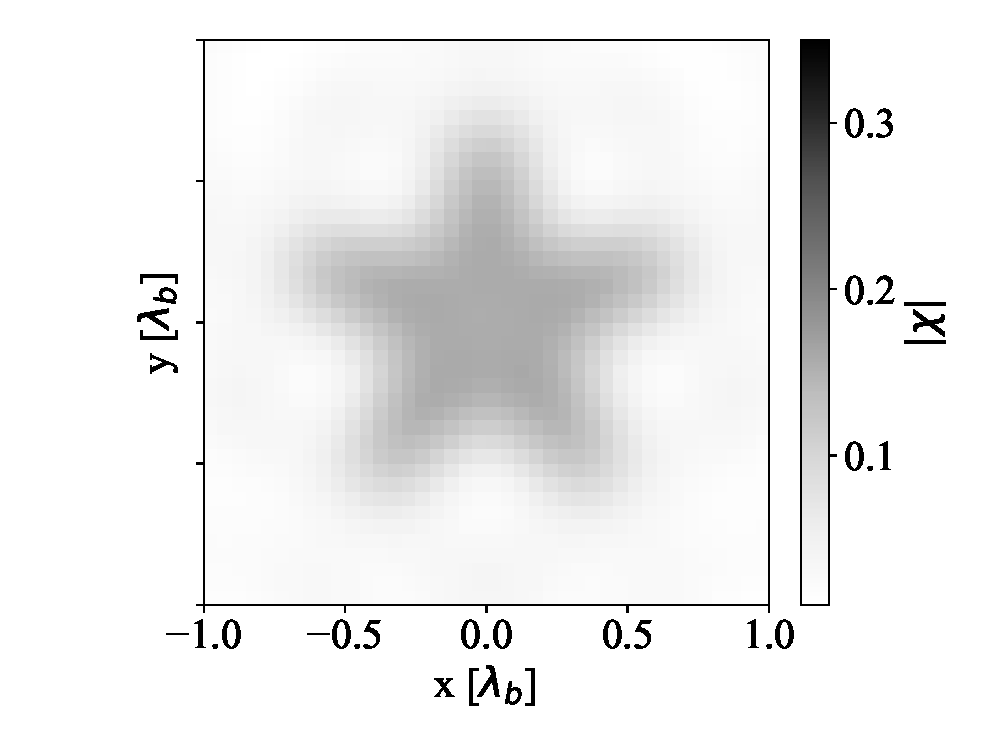
\includegraphics[width=0.3\textwidth]{./experiments/shape/star/figs/4.eps}}
                \subfigure[SOM]{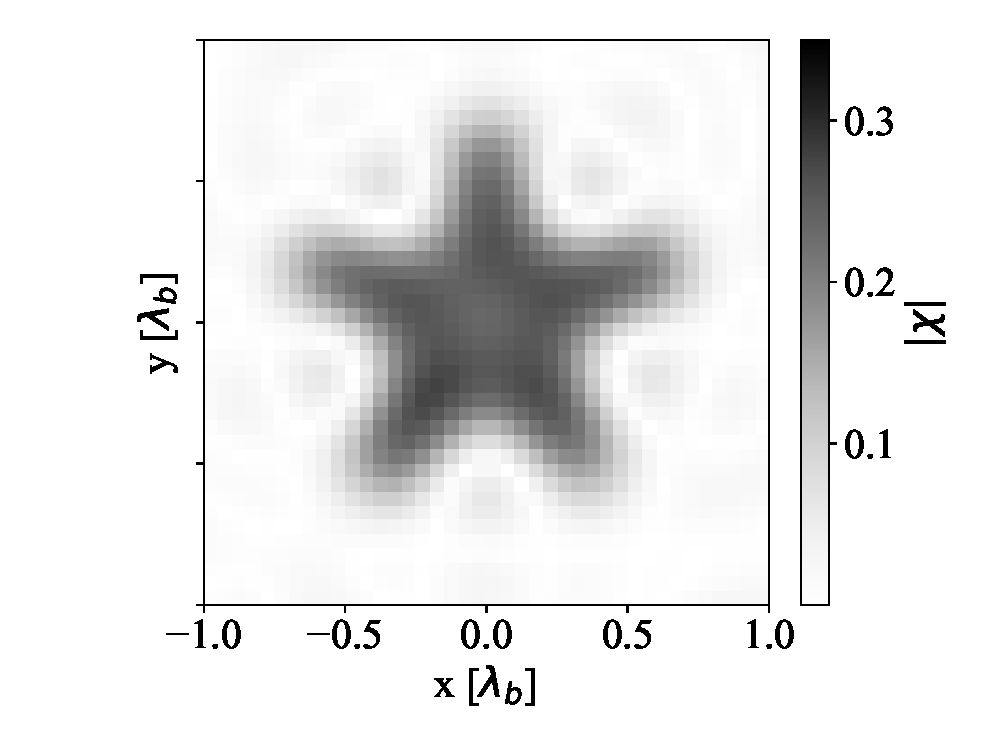
\includegraphics[width=0.3\textwidth]{./experiments/shape/star/figs/5.eps}}
                \caption{Shape recovering study, single scatterer: ground-truth and reconstructed images by each algorithm.}
                \label{fig:shape:single:recons}
            \end{figure*}
    
            Table \ref{tab:star} summarizes the results of the shape error indicator for each algorithm. The results indicate that BIM and SOM achieved the best performance, while CSI, LSM and OSM performed similarly. This is consistent with the observations from Fig. \ref{fig:shape:single:recons}, since the quantitative methods had a greater ability to capture the object's contours compared to the qualitative methods. This was not true for CSI, which, due to its greater difficulty in quantifying the object's contrast, had more difficulty in capturing the object's contours.           

            \begin{table}[!htb]
                \centering
                \renewcommand{\arraystretch}{1.5}
                \caption{Shape recovering study, single scatterer: shape error indicator $\zeta_S$ for each algorithm.}
                \label{tab:star}
                \begin{tabular}{cccccc}
                    Method & LSM & OSM & BIM & CSI & SOM \\\hline
                    $\zeta_S$ (\%) & 29.2 & 24.5 & 14.9 & 26.3 & 15.4 \\
                \end{tabular}   
            \end{table}
        
        \subsubsection{Varying contrast}\label{sec:results:shape:varying}

            Another type of study that can complement the analysis of algorithm performance in object geometry reconstruction is the observation of indicator performance with varying object contrast. Specifically, for a given scatterer, as its contrast value increases, the DNL increases, and consequently, algorithms may lose performance since the problem becomes more challenging. To demonstrate this relationship, the same scatterer from the previous study was considered with identical scenario configurations. The only modification was that the original image resolution was increased to 160$\times$160 pixels to ensure precision in field calculations for high contrast scenarios. 

            The scatterer was reconstructed using five contrast values: 0.25, 0.5, 0.75, 1.0, and 1.5. Fig. \ref{fig:shape:vary:dnl} shows the corresponding DNL for each contrast value. For this study, the OSM and SOM methods were employed with the same configurations as the previous study. While the method parameters could be optimized for each contrast value, they were kept constant across all contrast values to demonstrate the indicator's applicability in a controlled manner.

            \begin{figure*}[!htb]
                \centering
                \subfigure[OSM, $\chi=0.25$]{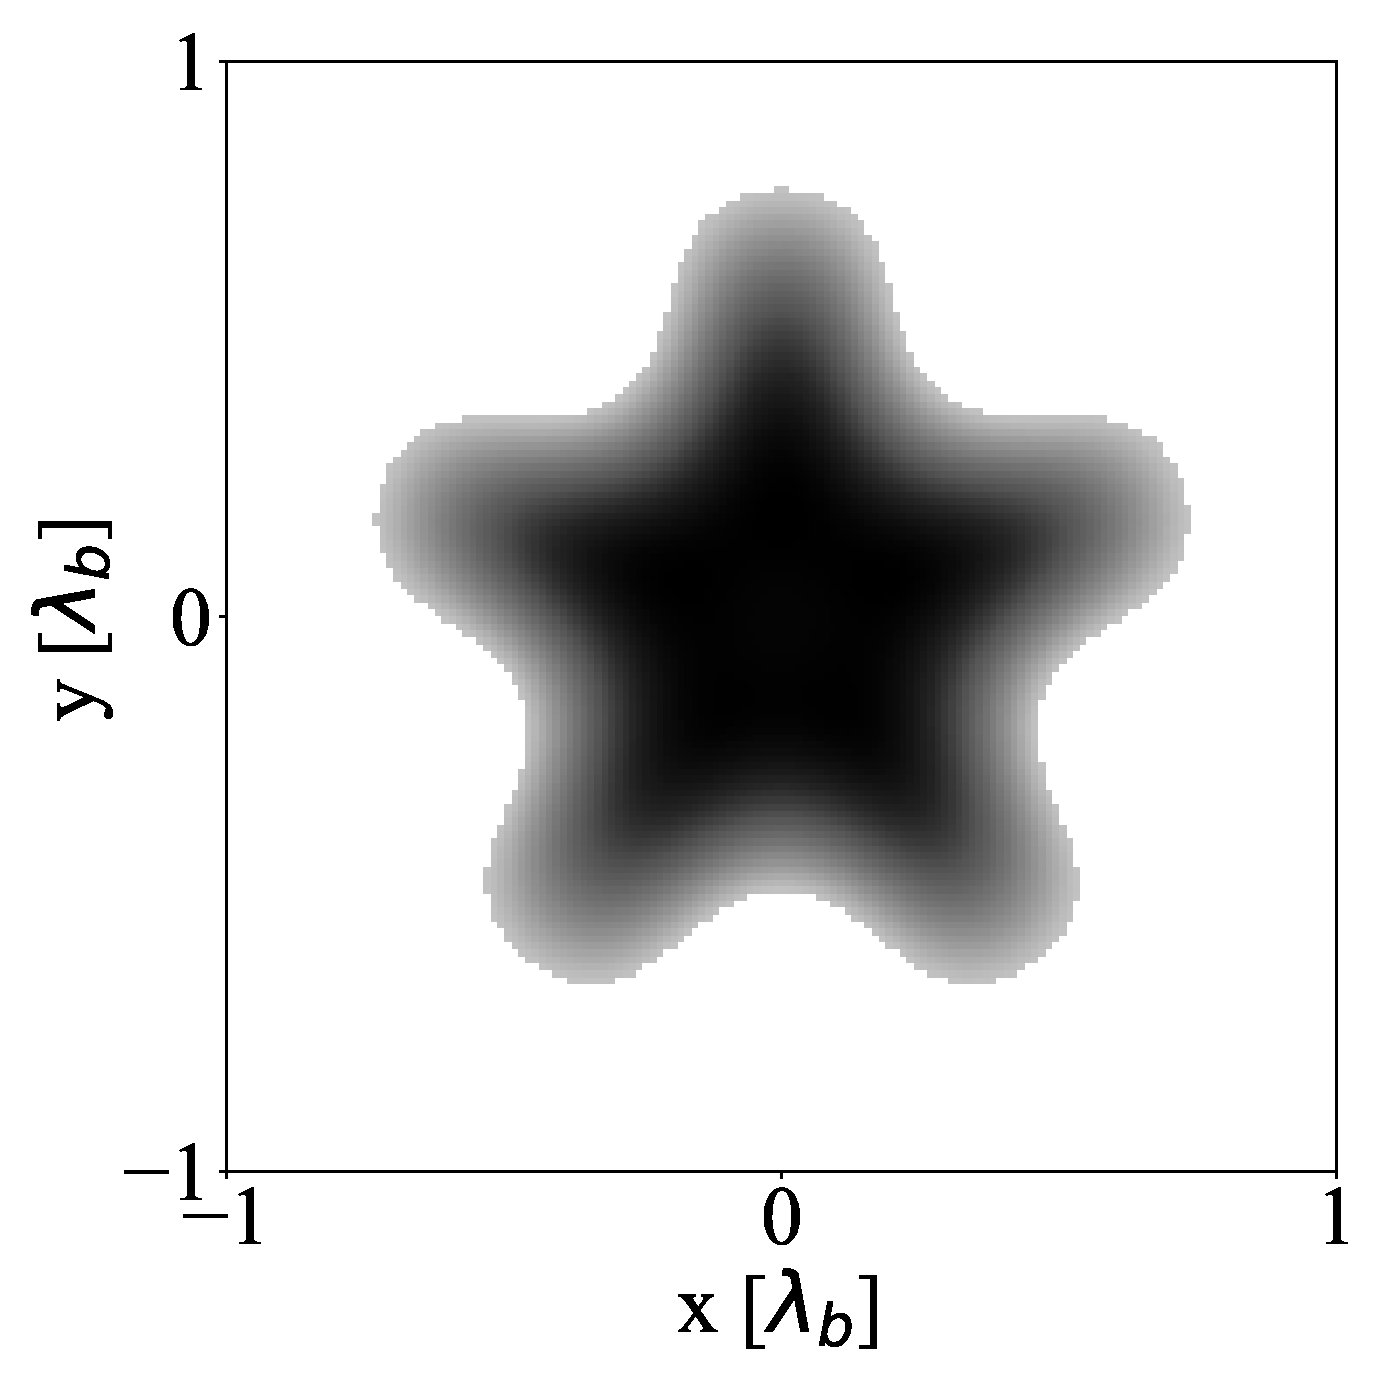
\includegraphics[height=1.2in]{./experiments/shape/vary/figs/osm_0.eps}}
                \subfigure[OSM, $\chi=0.5$]{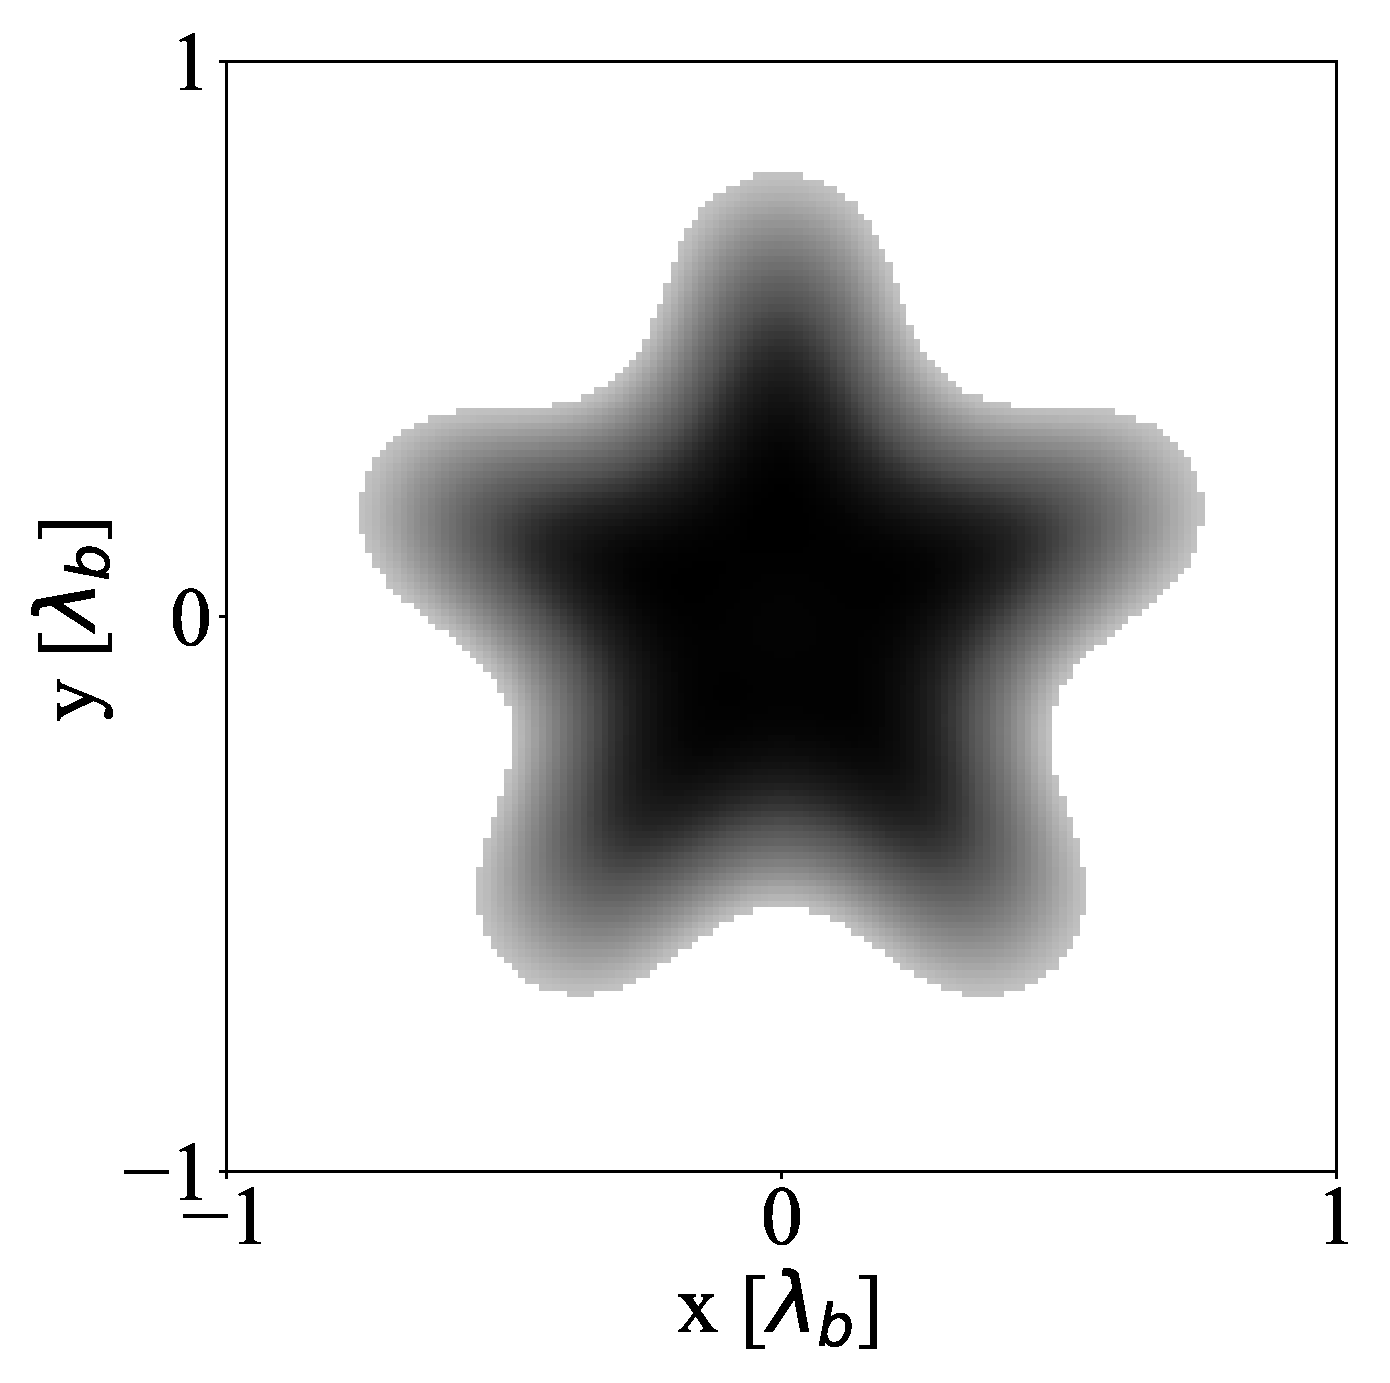
\includegraphics[height=1.2in]{./experiments/shape/vary/figs/osm_1.eps}}
                \subfigure[OSM, $\chi=0.75$]{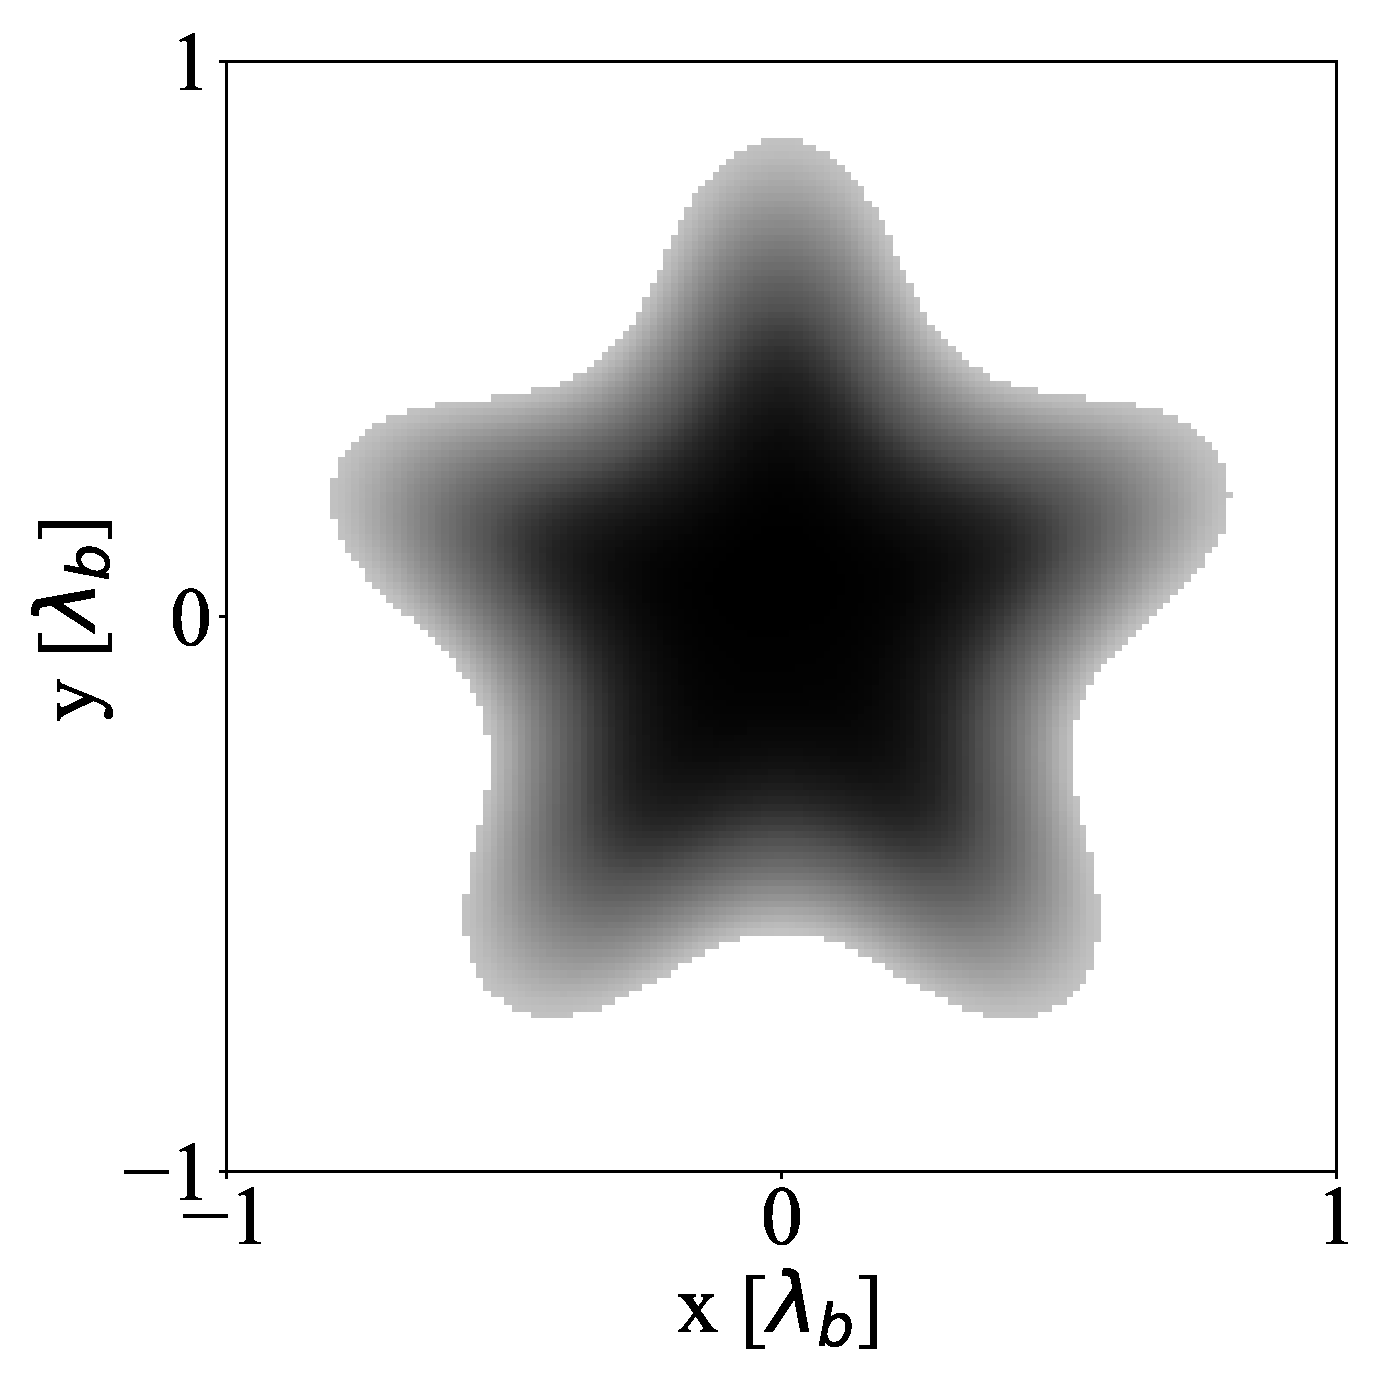
\includegraphics[height=1.2in]{./experiments/shape/vary/figs/osm_2.eps}}
                \subfigure[OSM, $\chi=1$]{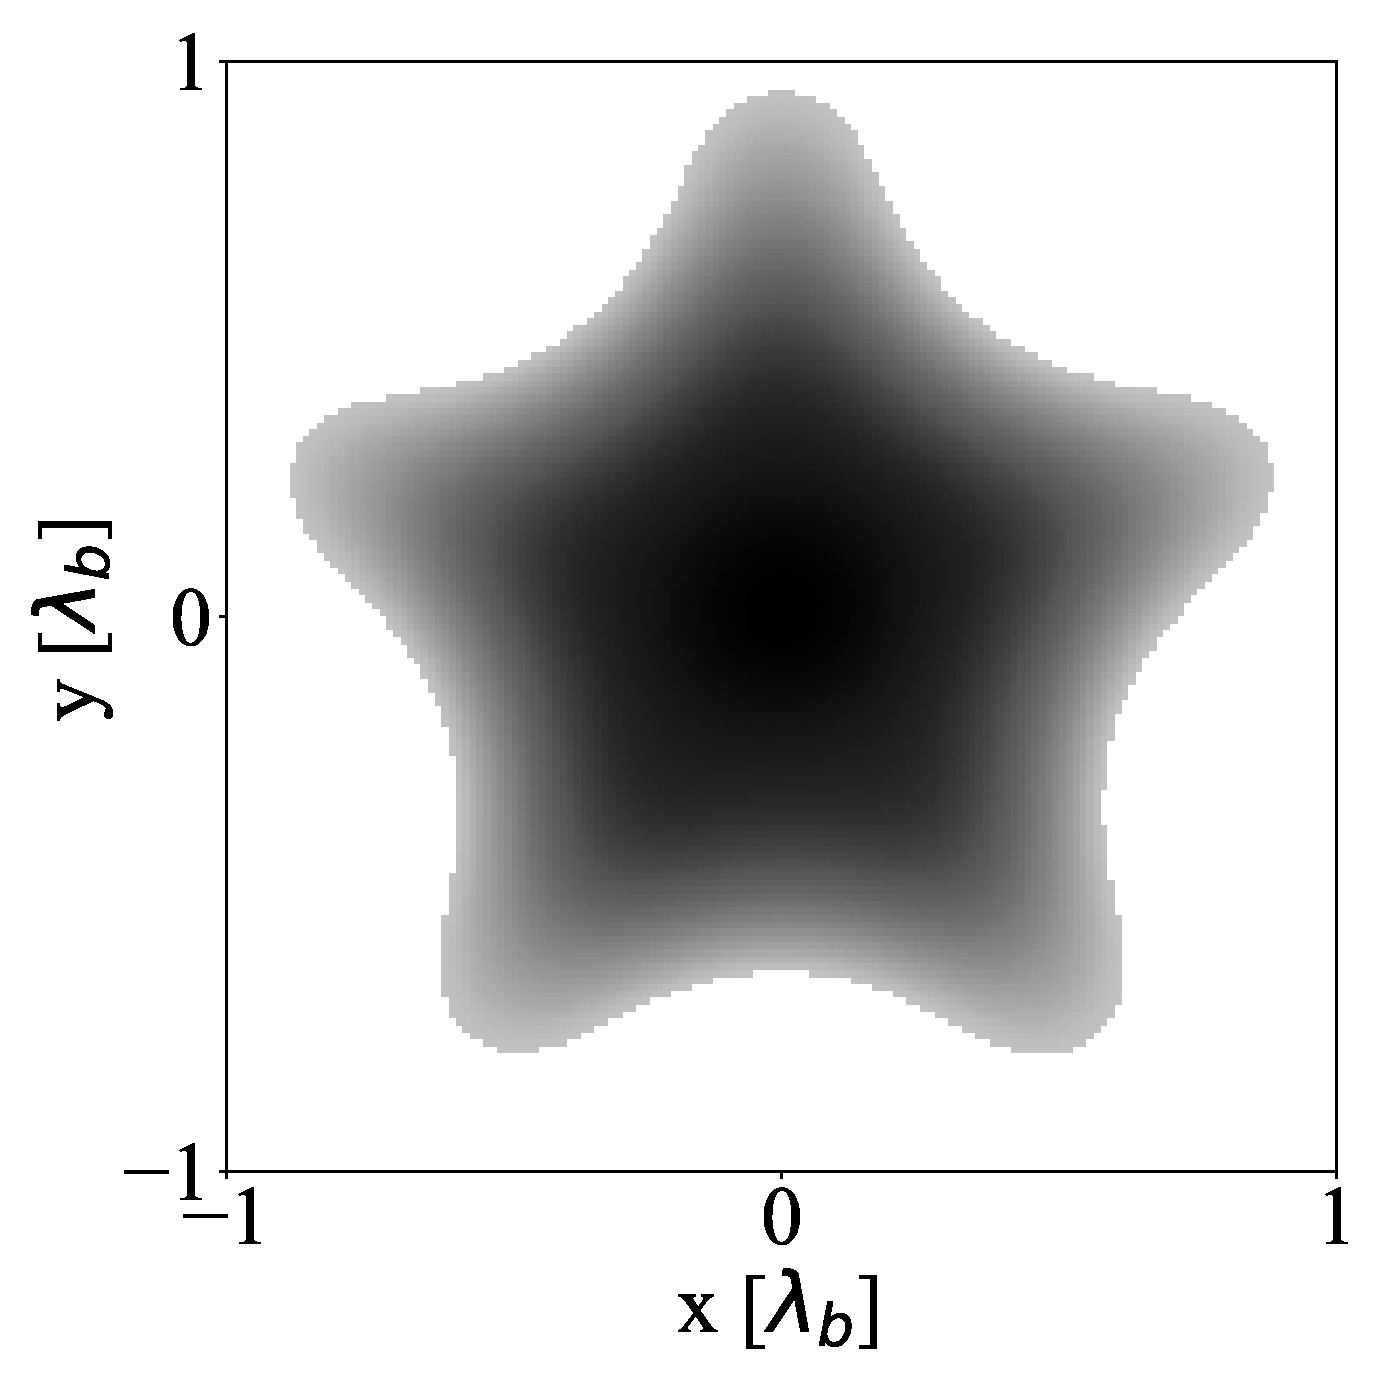
\includegraphics[height=1.2in]{./experiments/shape/vary/figs/osm_3.eps}}
                \subfigure[OSM, $\chi=1.5$]{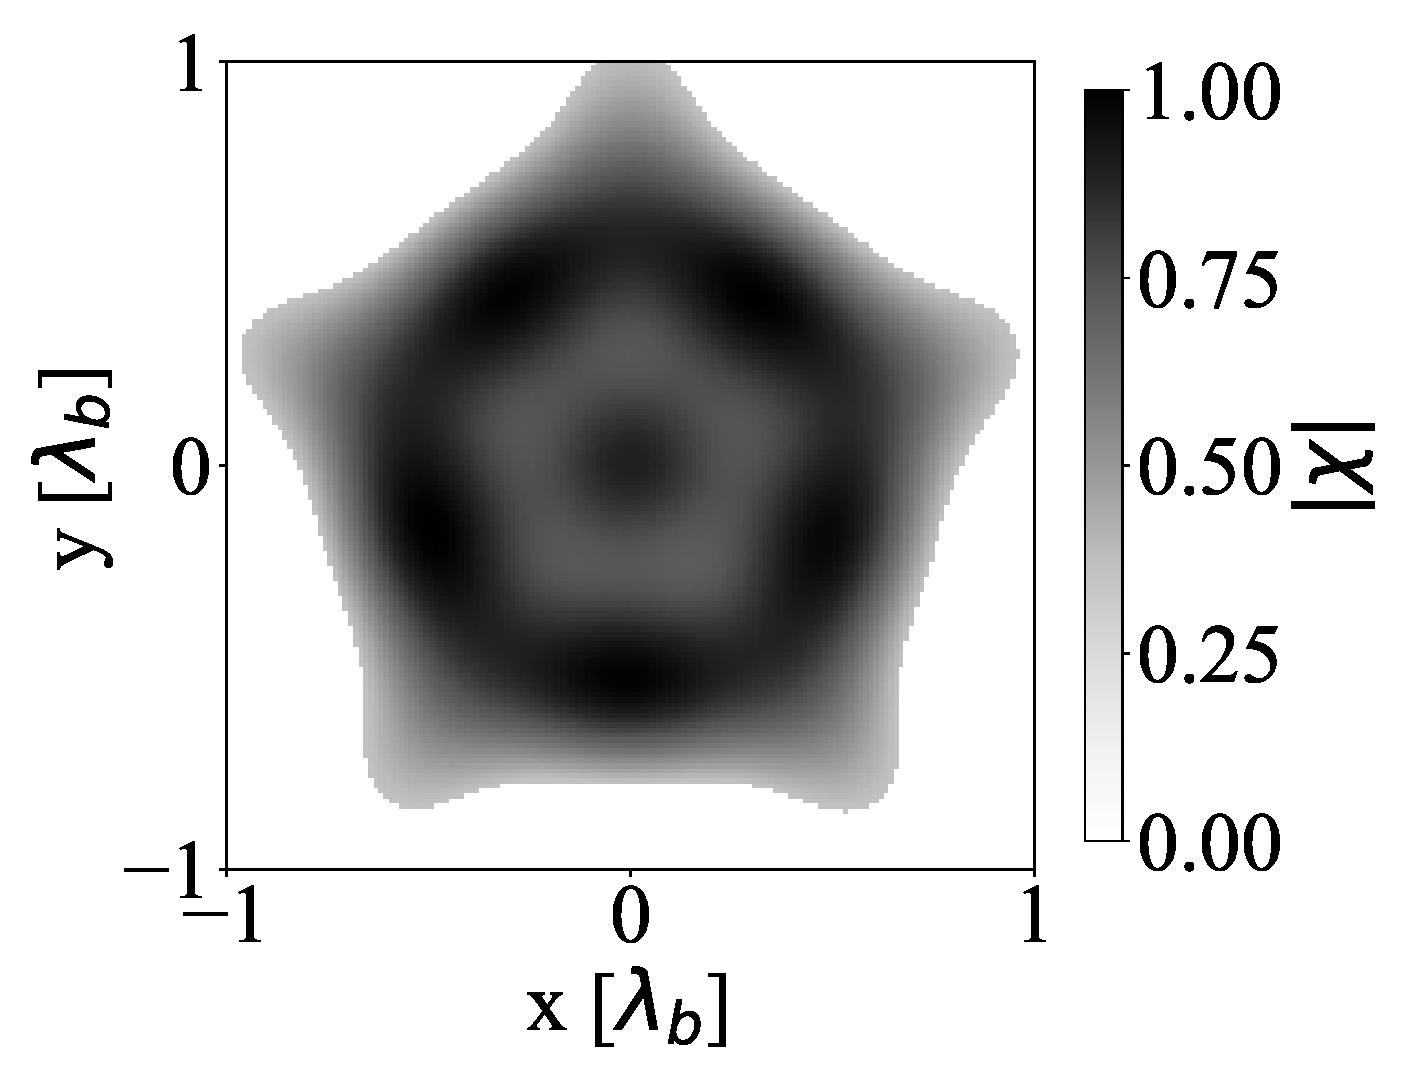
\includegraphics[height=1.2in]{./experiments/shape/vary/figs/osm_4.eps}} \\
                \subfigure[SOM, $\chi=0.25$]{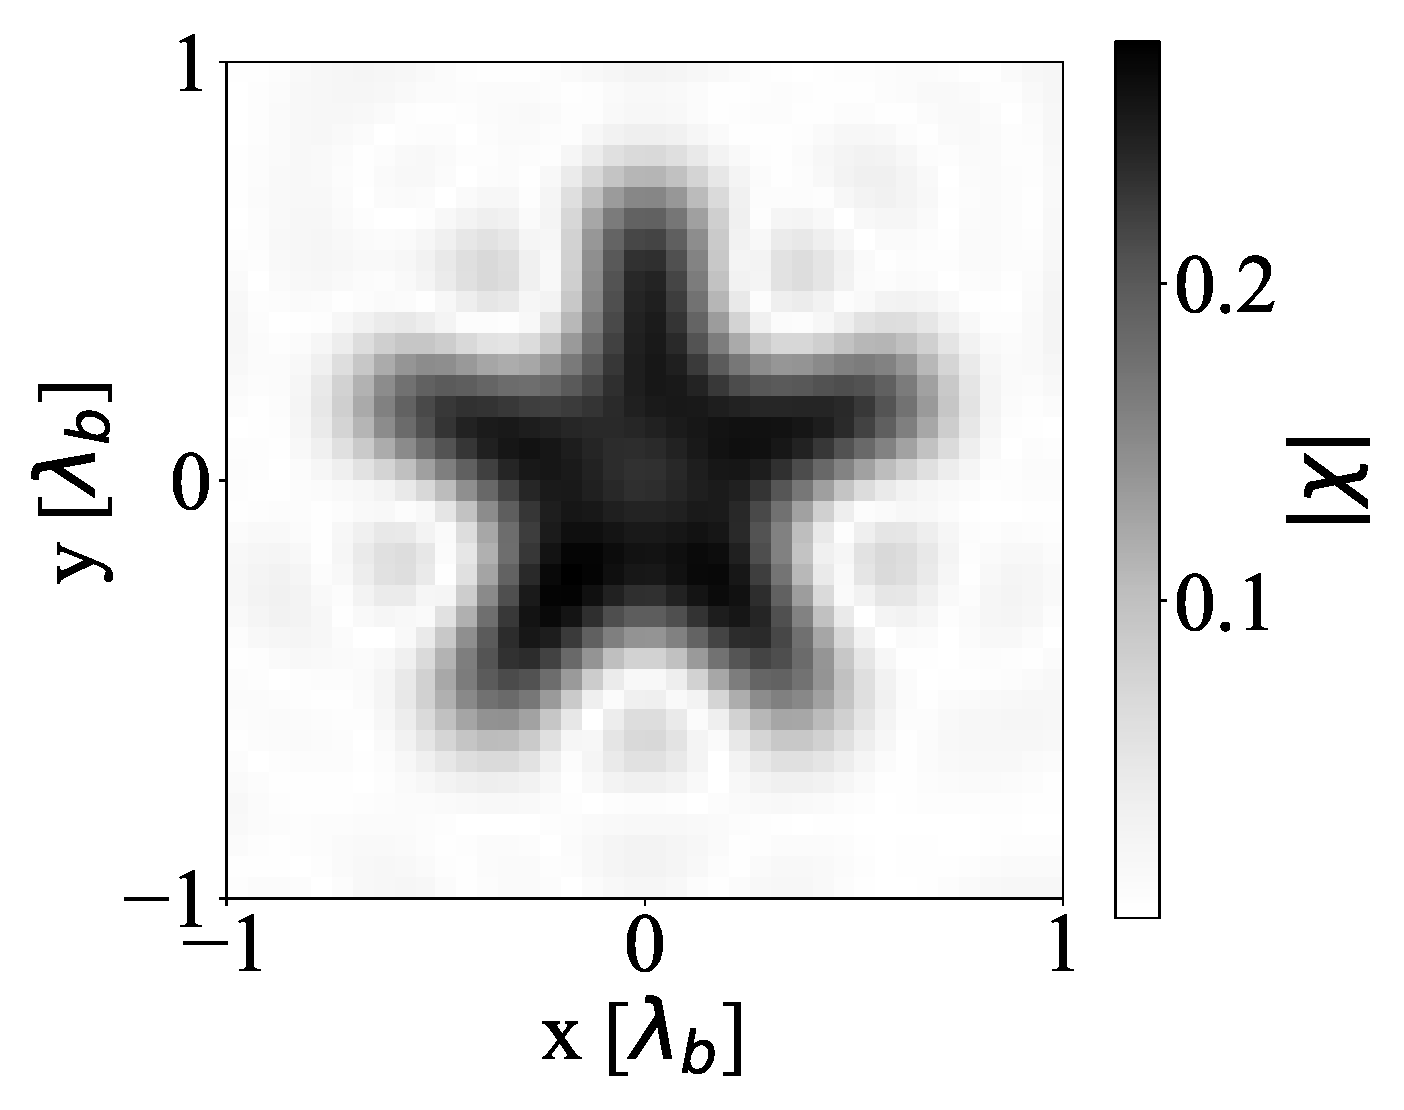
\includegraphics[height=1.in]{./experiments/shape/vary/figs/som_0.eps}}
                \subfigure[SOM, $\chi=0.5$]{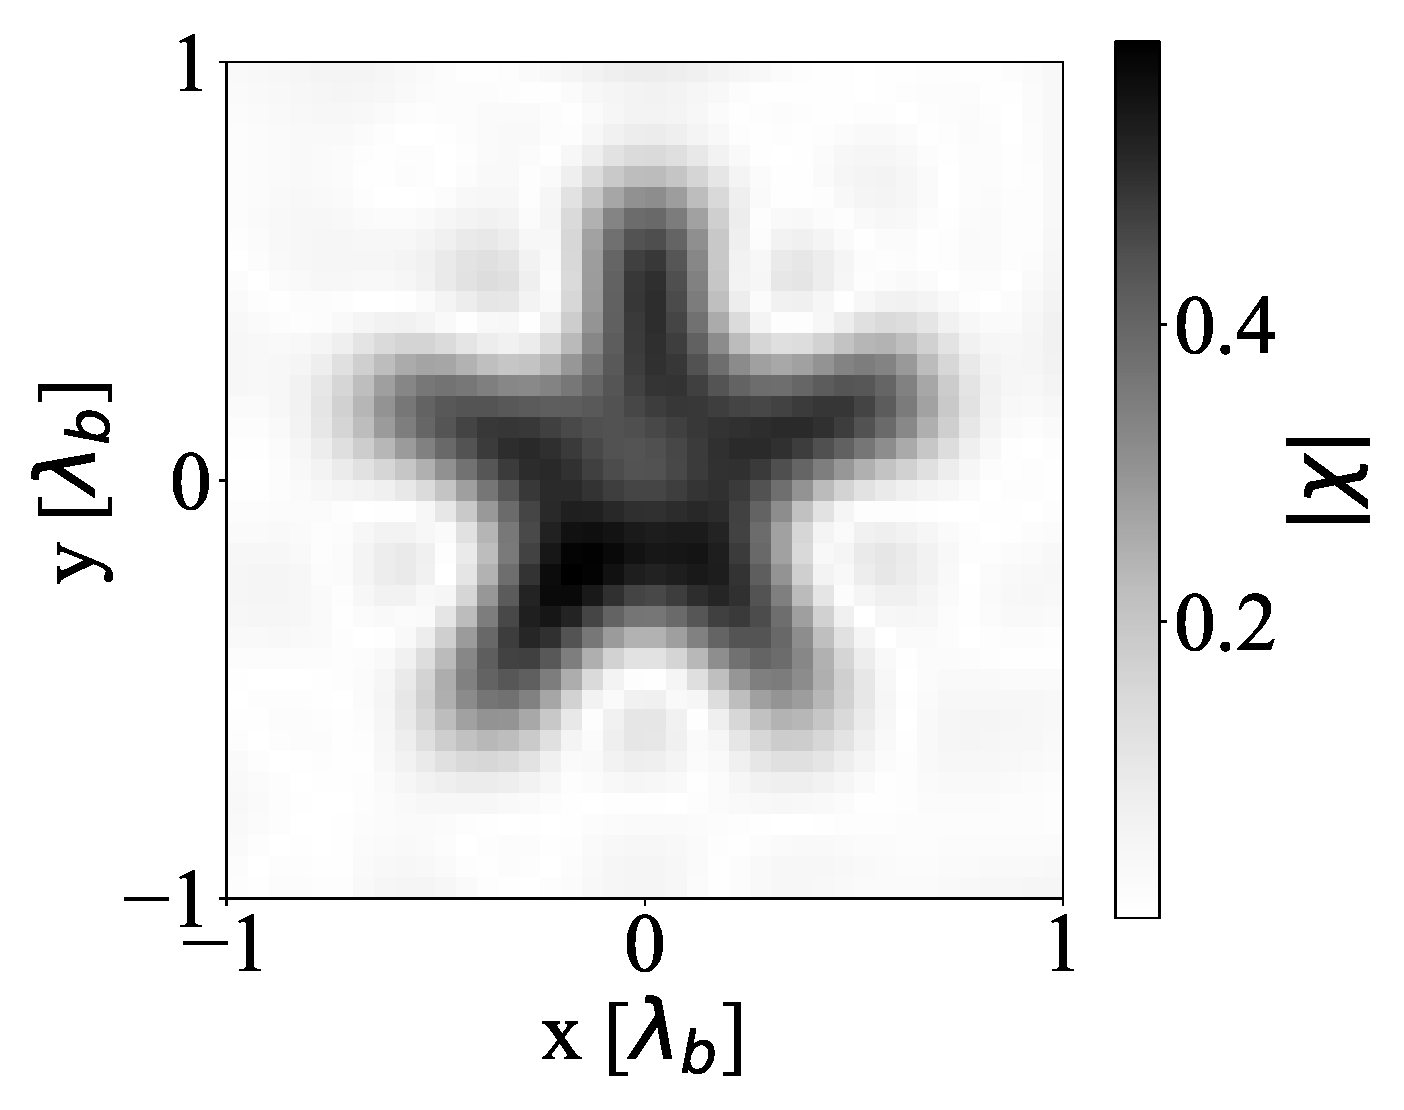
\includegraphics[height=1.in]{./experiments/shape/vary/figs/som_1.eps}}
                \subfigure[SOM, $\chi=0.75$]{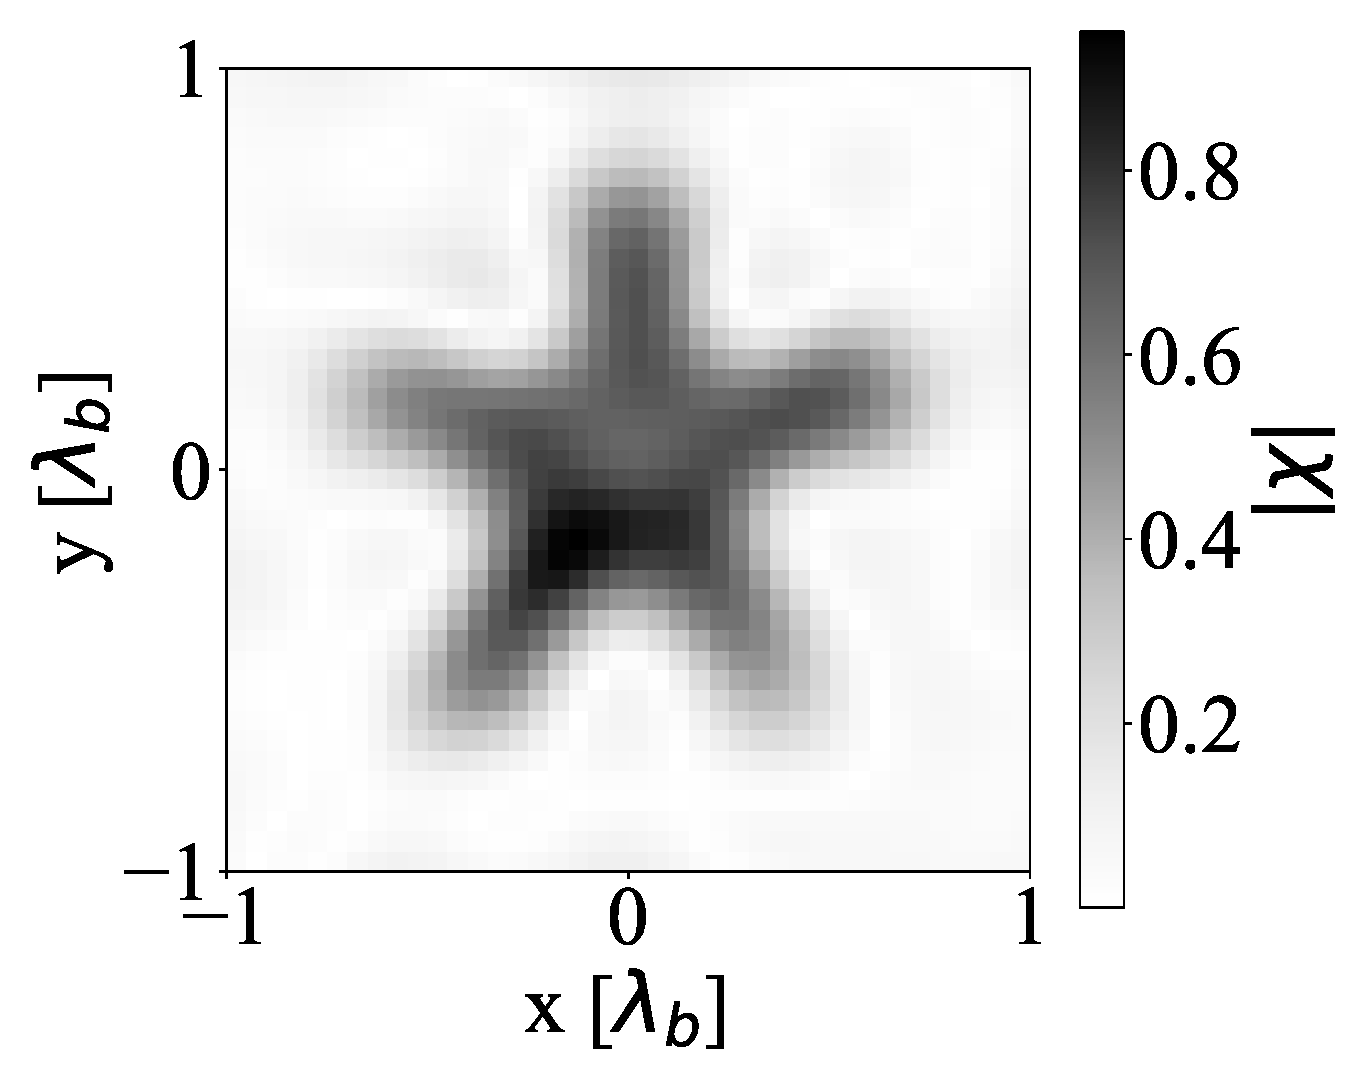
\includegraphics[height=1.in]{./experiments/shape/vary/figs/som_2.eps}}
                \subfigure[SOM, $\chi=1$]{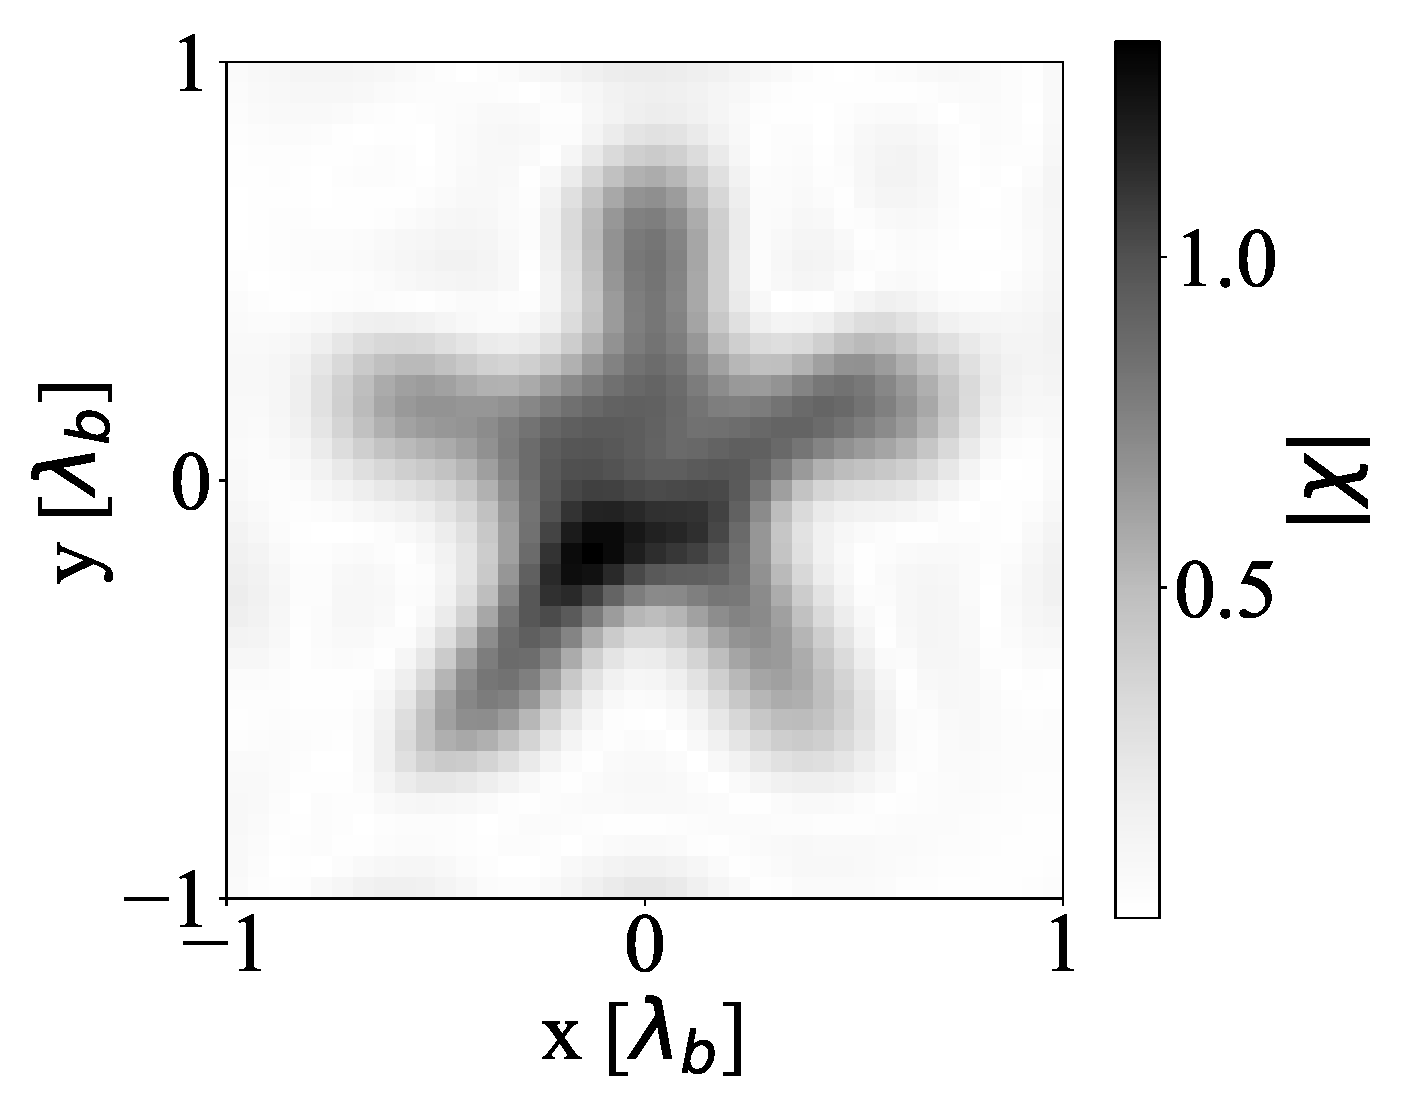
\includegraphics[height=1.in]{./experiments/shape/vary/figs/som_3.eps}}
                \subfigure[SOM, $\chi=1.5$]{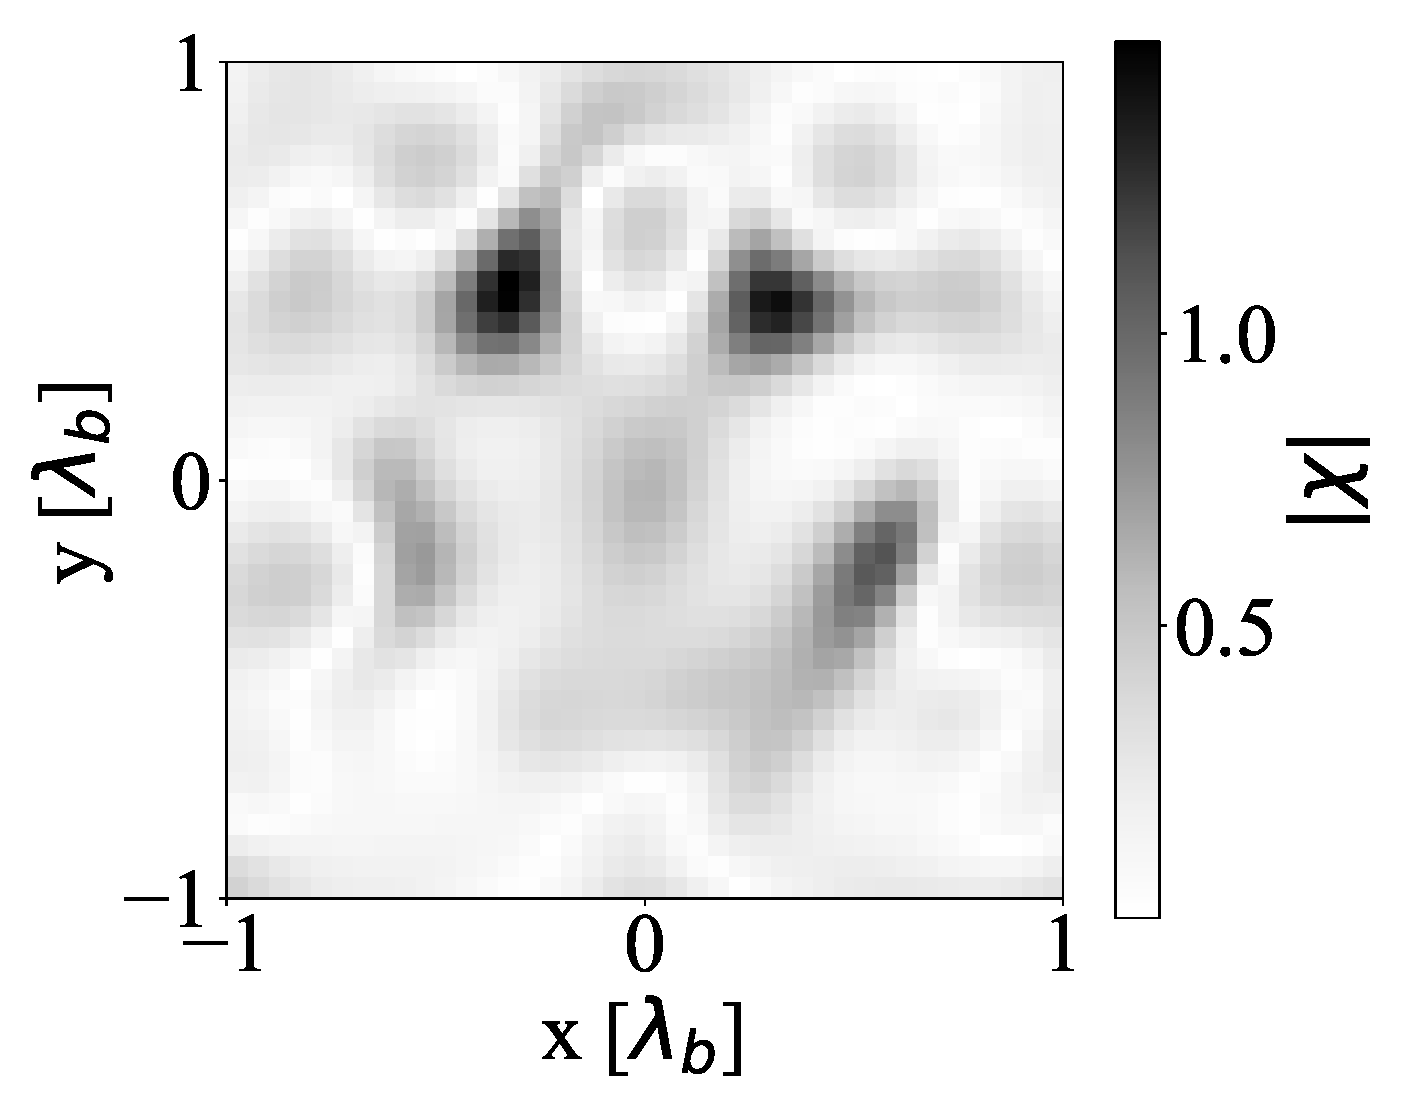
\includegraphics[height=1.in]{./experiments/shape/vary/figs/som_4.eps}}
                \caption{Shape recovering study, varying contrast: reconstructed images by OSM and SOM for different contrast values.}
                \label{fig:shape:vary:recons}
            \end{figure*}

            Fig. \ref{fig:shape:vary:recons} shows the images reconstructed by OSM and SOM for each contrast value. As expected, reconstruction precision decreased with increasing contrast, reaching a point where the geometry was no longer correctly recovered for the highest contrast value (1.5), particularly in the case of SOM. Notably, SOM was able to estimate the scatterer's contrast with reasonable precision up to $\chi = 1$, where the DNL is approximately 2.

            Fig. \ref{fig:shape:vary:indicators:zeta_s} presents the shape error indicator $\zeta_S$ for both OSM and SOM methods. The results demonstrate that the shape error increases proportionally with contrast value, which is consistent with the expected algorithmic behavior. Furthermore, for $\chi = 1.5$, the indicator $\zeta_S$ exceeds 100\%, indicating that the number of incorrectly classified pixels surpasses the number of pixels composing the scatterer in the original image. This observation aligns with the finding that geometry recovery fails at this contrast level. Additionally, the difference between the OSM and SOM indicators remains relatively constant up to $\chi = 1$.

            \begin{figure}[!htb]
                \centering
                \subfigure[]{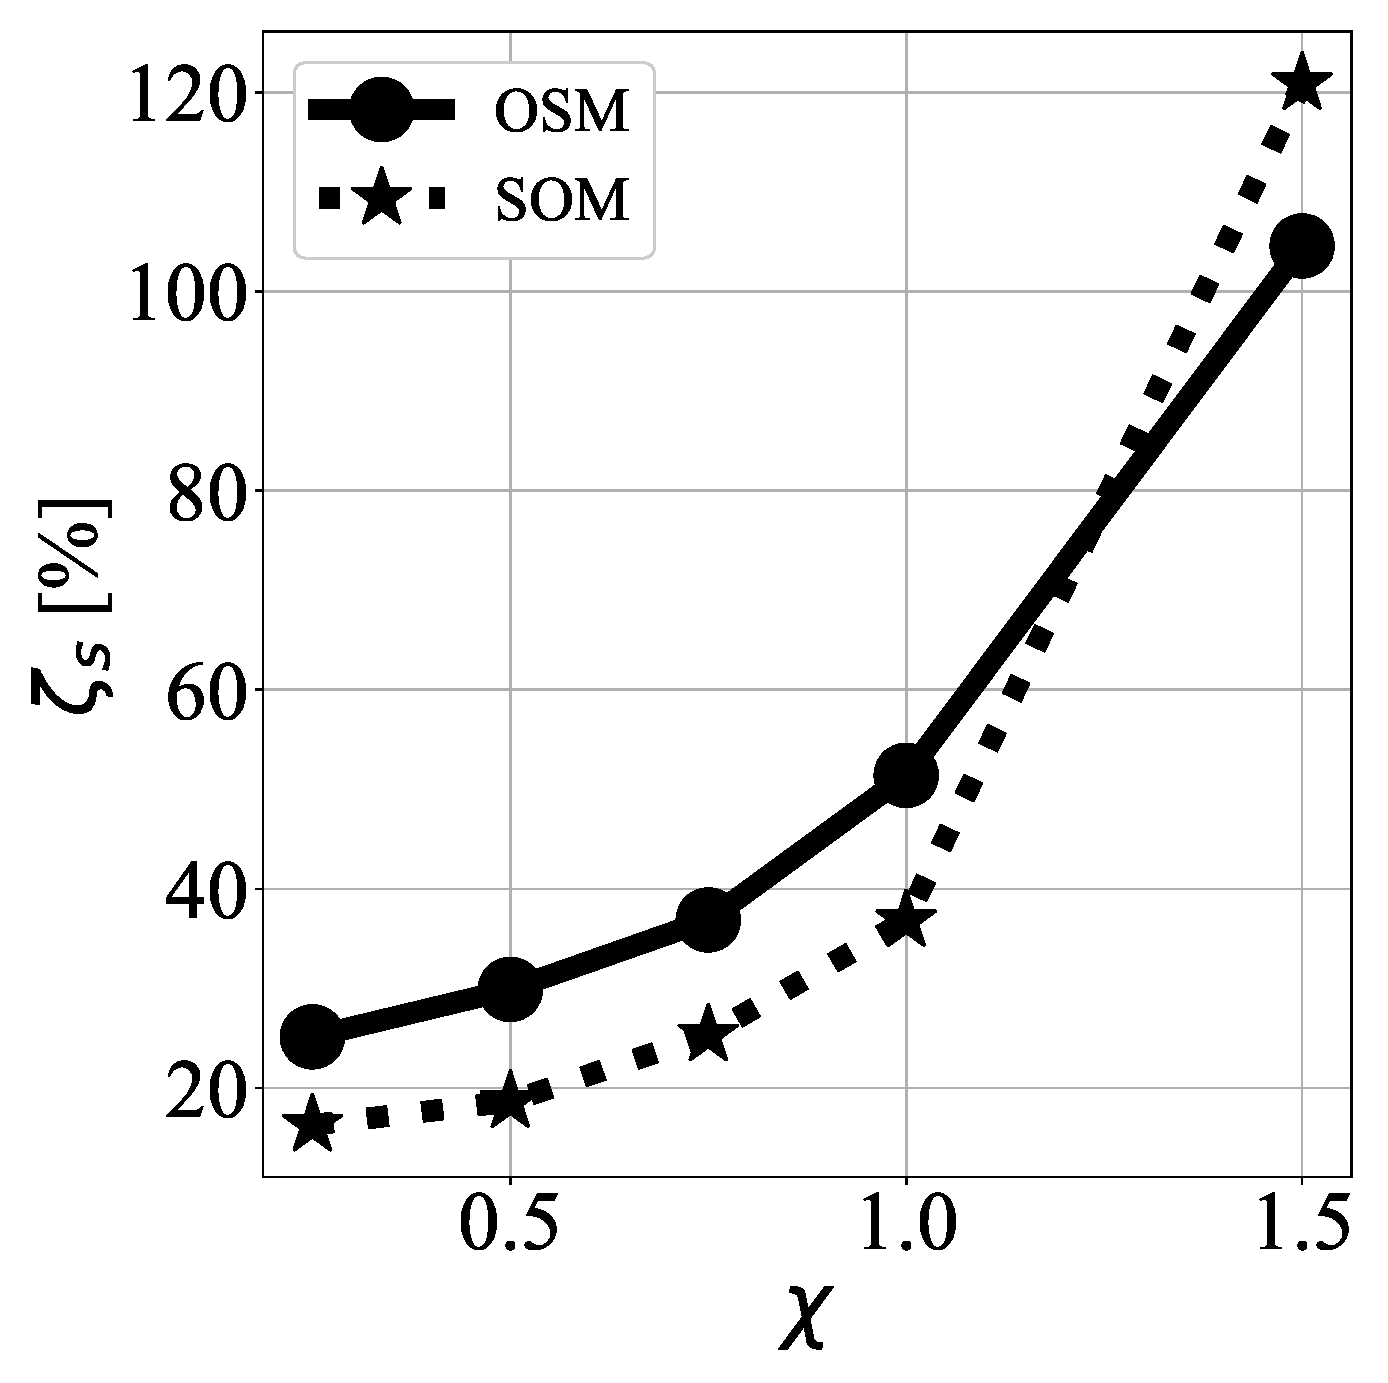
\includegraphics[width=0.48\columnwidth]{./experiments/shape/vary/figs/zeta_s.eps}\label{fig:shape:vary:indicators:zeta_s}} \hspace{0.01\columnwidth}
                \subfigure[]{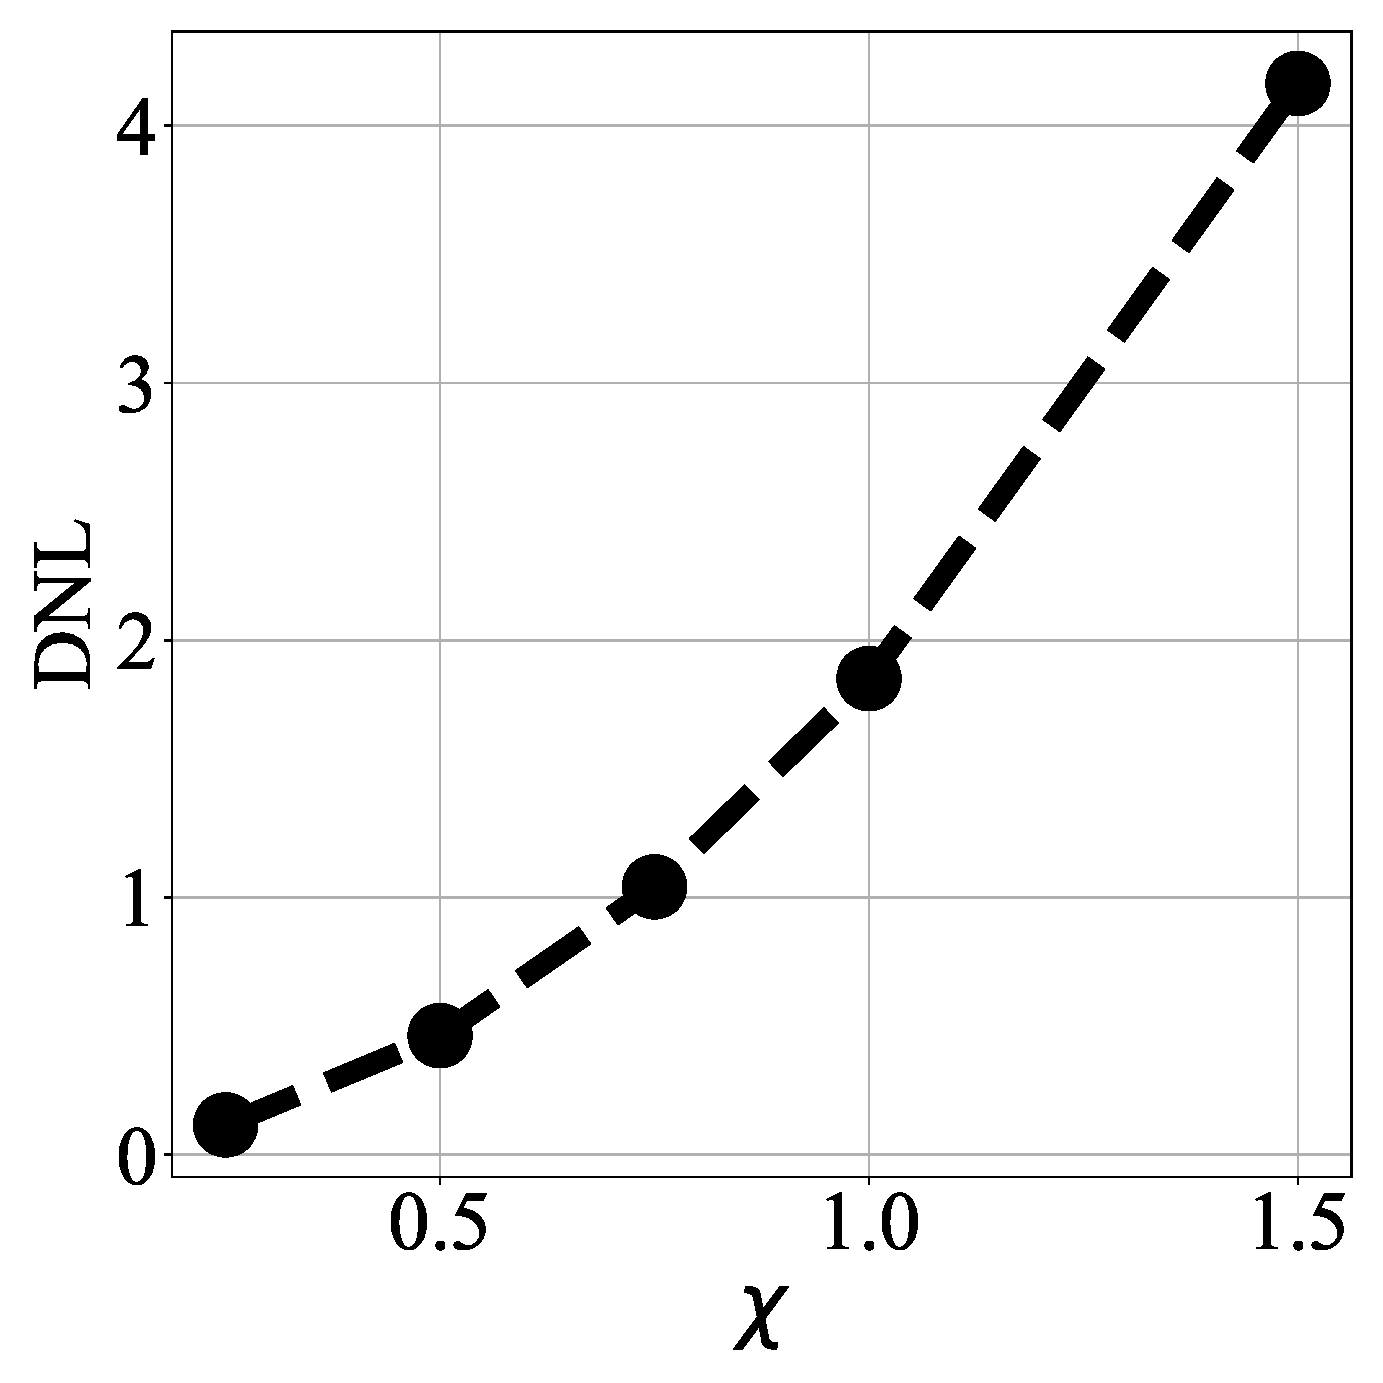
\includegraphics[width=0.48\columnwidth]{./experiments/shape/vary/figs/dnl.eps}\label{fig:shape:vary:dnl}}
                \caption{Shape recovering study, varying contrast: (a) shape error indicator $\zeta_S$ for OSM and SOM; (b) Degree of Nonlinearity (DNL) for each contrast value.}
                \label{fig:shape:vary:indicators}
            \end{figure}

        \subsubsection{Average performance}\label{sec:results:shape:average}

            When comparing multiple algorithms, it is advantageous to conduct case studies using test sets that represent specific problem classes. This approach enables the measurement and statistical comparison of average algorithm performance, thereby supporting more robust and reliable conclusions regarding their relative effectiveness.

            Following such an approach, an experiment was conducted to compare the LSM, OSM, BIM, CSI, and SOM algorithms. This experiment utilized 30 scatterer images with varying geometries to provide a more comprehensive assessment of algorithm performance across different shape configurations.

            The scatterers were randomly generated as polygons with 4 to 15 vertices, where the radius from the center to the farthest vertices ranged between 0.45$\lambda_b$ and 0.9$\lambda_b$. The contrast was fixed at 0.25 for all scatterers, and the data synthesis parameters from Section \ref{sec:results:shape:star} were maintained for consistency. 

            Due to the geometric variations, the DNL for each instance varies accordingly, as illustrated in Fig. \ref{fig:shape:average:dnl}. The median DNL exceeds the value from the experiment in Section \ref{sec:results:shape:star}, though both remain significantly below the threshold of 1, above which the Born Approximation becomes inapplicable \cite{bucci2001degree}. This experimental design enables the assessment of statistical evidence supporting the superiority of any algorithm within this problem class.

            \begin{figure}[!htb]
                \centering
                \subfigure[]{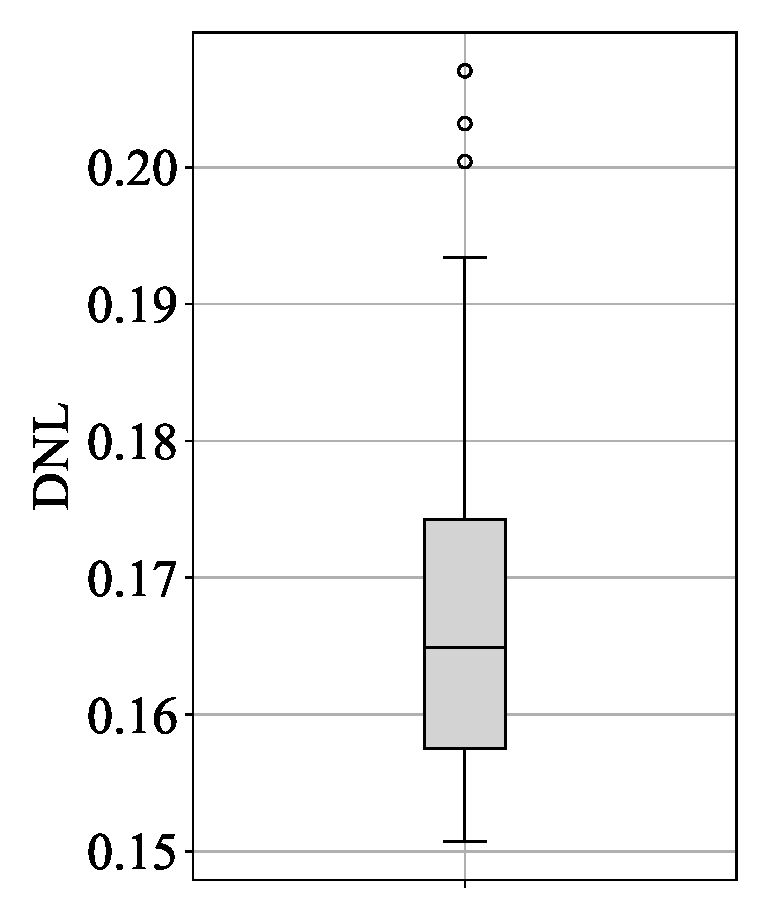
\includegraphics[width=.5\columnwidth]{./experiments/shape/average/figs/dnl.eps}\label{fig:shape:average:dnl}} \\
                \subfigure[]{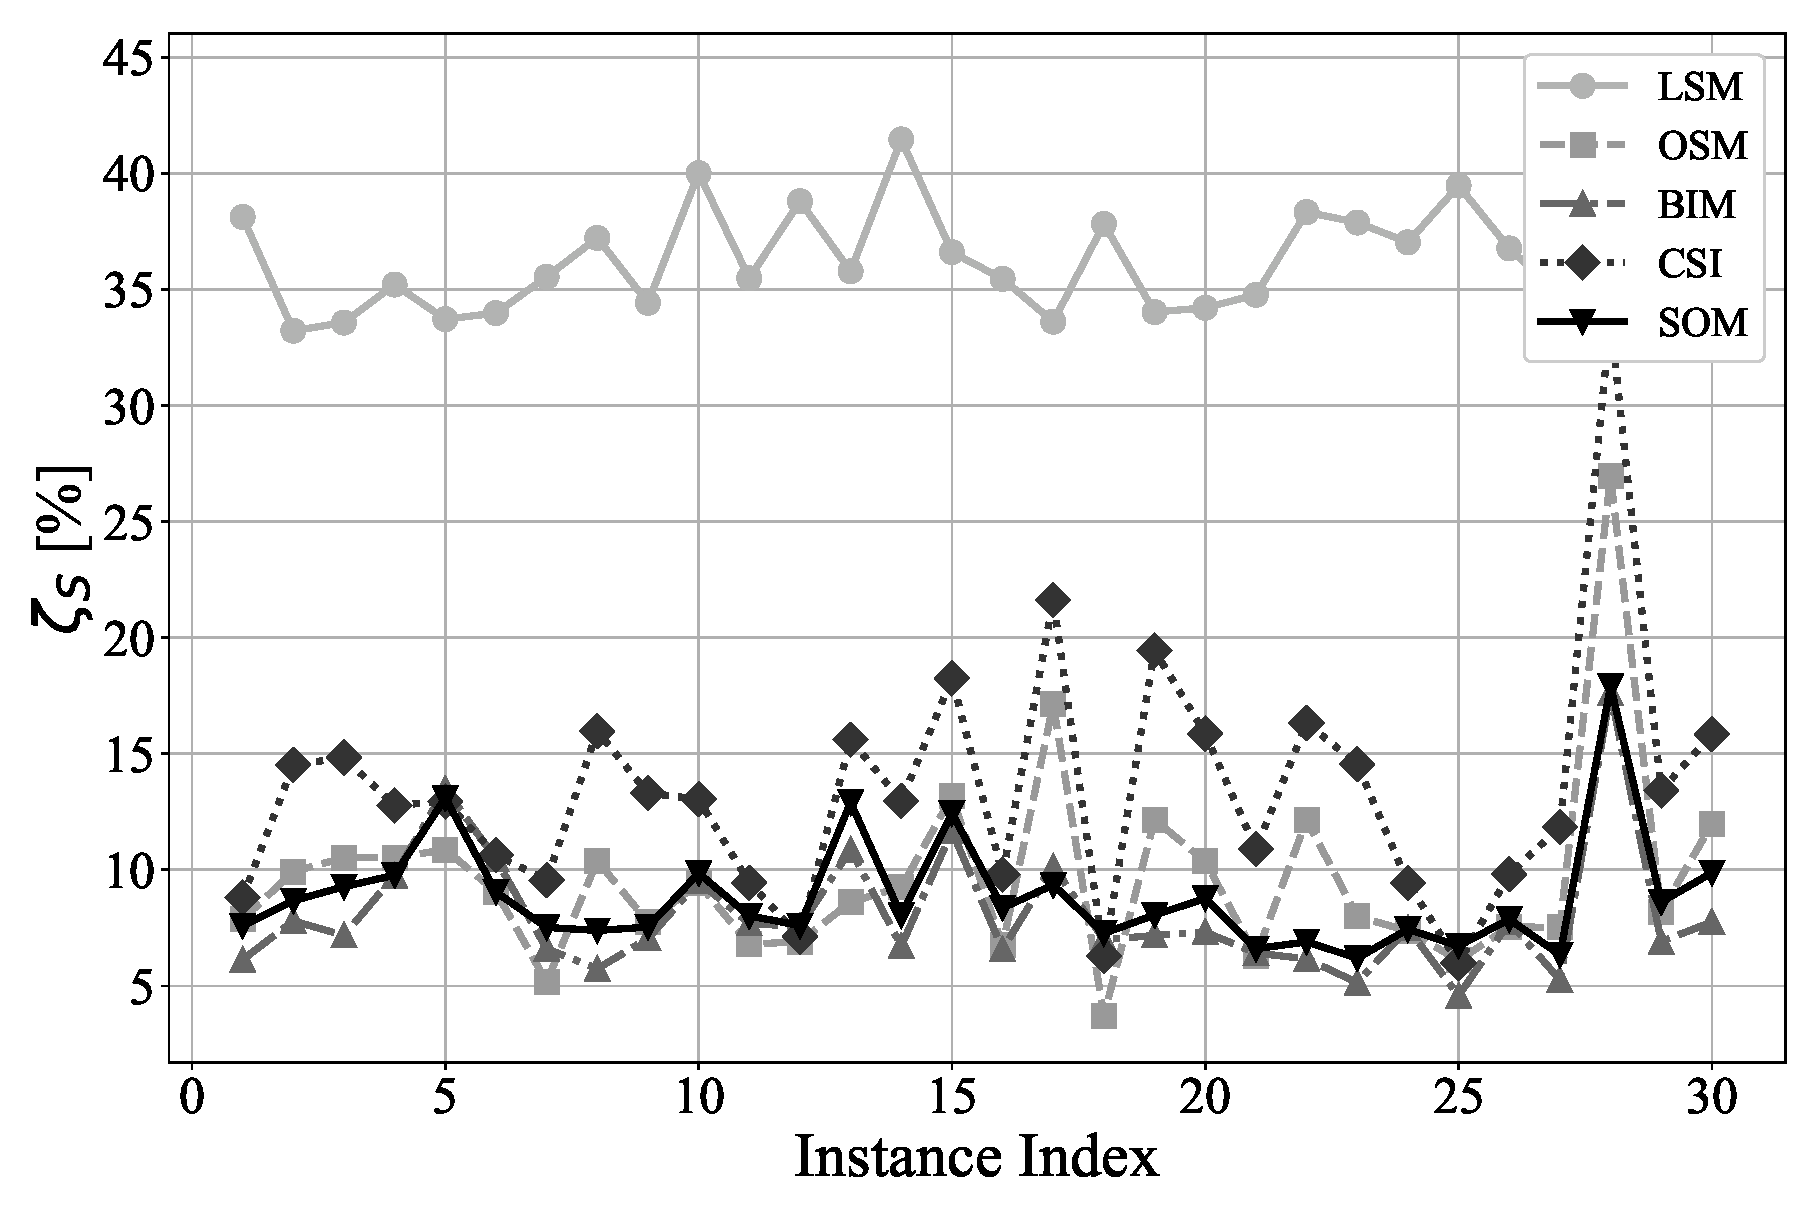
\includegraphics[width=\columnwidth]{./experiments/shape/average/figs/plot.eps}\label{fig:shape:average:zeta_s}}
                \caption{Shape recovering study, average performance: (a) Degree of Nonlinearity (DNL) for each scatterer; (b) shape error indicator $\zeta_S$ for each algorithm in each instance.}
                \label{fig:shape:average}   
            \end{figure}

            Fig. \ref{fig:shape:average:zeta_s} presents the shape error indicator $\zeta_S$ for each algorithm across all test instances. The results reveal a clear performance distinction when considering LSM, which demonstrates significantly worse performance compared to the other methods. Among the remaining algorithms, while overall performance levels appear similar, some patterns emerge: CSI exhibits higher error rates across a significant number of instances, whereas BIM demonstrates superior performance in a significant portion of the test cases.

            While Fig. \ref{fig:shape:average:zeta_s} provides initial insights into the results, statistical testing is important to validate the conclusions rigorously. To this end, Randomized Complete Block Design (RCBD) was applied to assess whether significant paired differences exist among the algorithms. RCBD is a statistical test which is used to evaluate significant paired differences between three or more related groups when the data meet the assumptions for parametric tests. In this context, the groups correspond to the algorithms, and the measurements are the $\zeta_S$ indicator values for each algorithm across all instances. Given that LSM demonstrated substantially inferior performance compared to the other algorithms, it was excluded from the statistical analysis to focus on the more competitive methods.

            After validating normality assumption, the p-value computed by RCBD result was less than $10^{-15}$, indicating that at least one pair of algorithms shows a significant mean paired difference. Subsequently, multiple paired T-Test with Bonferroni correction were applied to identify which algorithms have significant mean paired differences between them. The p-values obtained from these tests are presented in Table \ref{tab:shape:average:pvalue}. As shown in the table, the null hypothesis that algorithms have equal performance is rejected for all algorithm pairs, except for OSM-SOM, indicating that OSM and SOM do not exhibit a significant difference in their average performance.

            \begin{table*}
                \centering
                \renewcommand{\arraystretch}{1.5}
                \caption{Shape recovering study, average performance: $p$-values for the paired T-Test with Bonferroni correction.}
                \label{tab:shape:average:pvalue}
                \begin{tabular}{ccccccc}
                    Pairs & OSM-BIM & OSM-CSI & OSM-SOM & BIM-CSI & BIM-SOM & CSI-SOM \\\hline
                    $p$-value & $<10^{-2}$ & $<10^{-11}$ & 0.15 & $<10^{-7}$ & $<10^{-4}$ & $<10^{-6}$ \\  
                \end{tabular}
            \end{table*}

            To complement the analysis, Fig. \ref{fig:shape:average:confidence_intervals} presents the 95\% confidence intervals for the mean paired differences of the shape error indicator $\zeta_S$ for each algorithm pair. As observed, the differences consistently favor BIM, providing evidence for BIM's superiority over the other algorithms. Additionally, CSI performs significantly worse than both BIM, OSM and SOM. However, all differences in average performance are less than 7\%.

            Furthermore, it is noteworthy that BIM also achieved the best performance in the study from Section \ref{sec:results:shape:star}. However, while the difference between SOM and OSM was significant in the experiment from Section \ref{sec:results:shape:star}, this benchmarking study provided evidence for performance equivalence between these two methods. In other words, if conclusions were drawn based solely on the case study, this could lead to a misconception about the performance of these two methods in this problem configuration. Therefore, this reinforces the importance of conducting benchmarking studies combined with statistical analyses to obtain more robust conclusions about algorithm performance.

            \begin{figure}
                \centering
                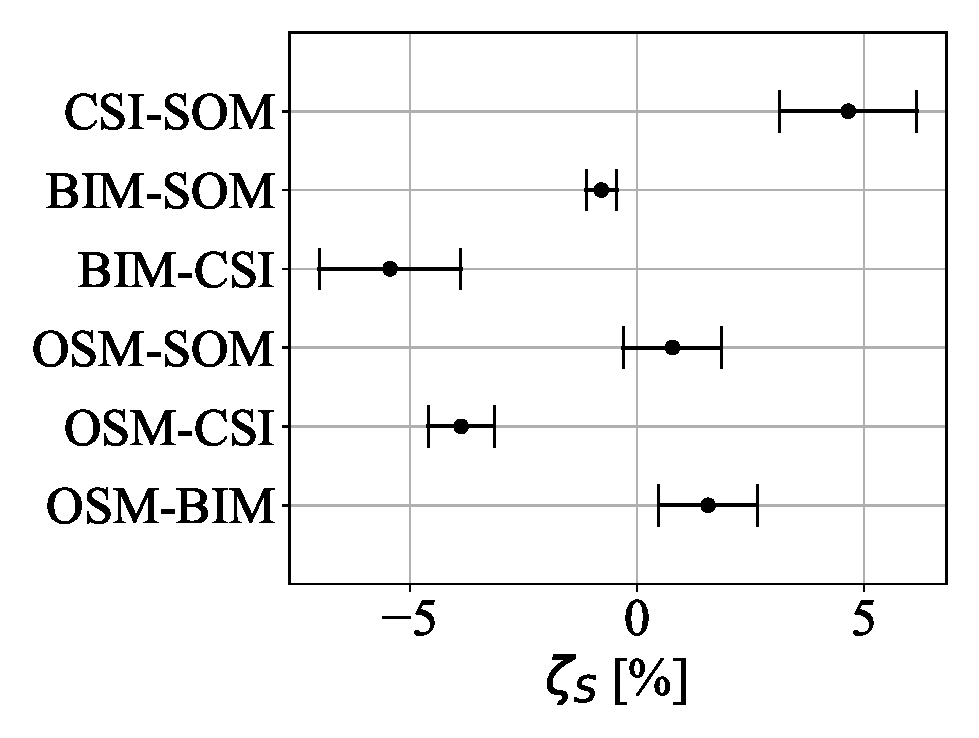
\includegraphics[width=.8\columnwidth]{./experiments/shape/average/figs/confidence_intervals.eps}
                \caption{Shape recovering study, average performance: Confidence intervals (95\%) for the shape error indicator $\zeta_S$ for each pair of algorithms.}
                \label{fig:shape:average:confidence_intervals}
            \end{figure}

        \subsubsection{Indicator Comparison}\label{sec:results:shape:indicatorcomparison}

            To further illustrate the application of the proposed shape error indicator, an experiment was conducted to compare its behavior with other commonly used indicators in the literature. Specifically, the Root Mean Square Error (RMSE) between the original and reconstructed images, denoted as $\zeta_{\epsilon PAD}$ according to \cite{batista2025eispy2d}, and the Structural Similarity Index Measure (SSIM) \cite{wang2004image} were considered for comparison.

            The experiment involved reconstructing a star-shaped scatterer, as described in Section \ref{sec:results:shape:star}, using the SOM algorithm. The reconstruction process was performed over 100 iterations, with images saved at iterations 10, 20, 30, and 100. 

            \begin{figure*}[!htb]
                \centering
                \subfigure[Ground-Truth]{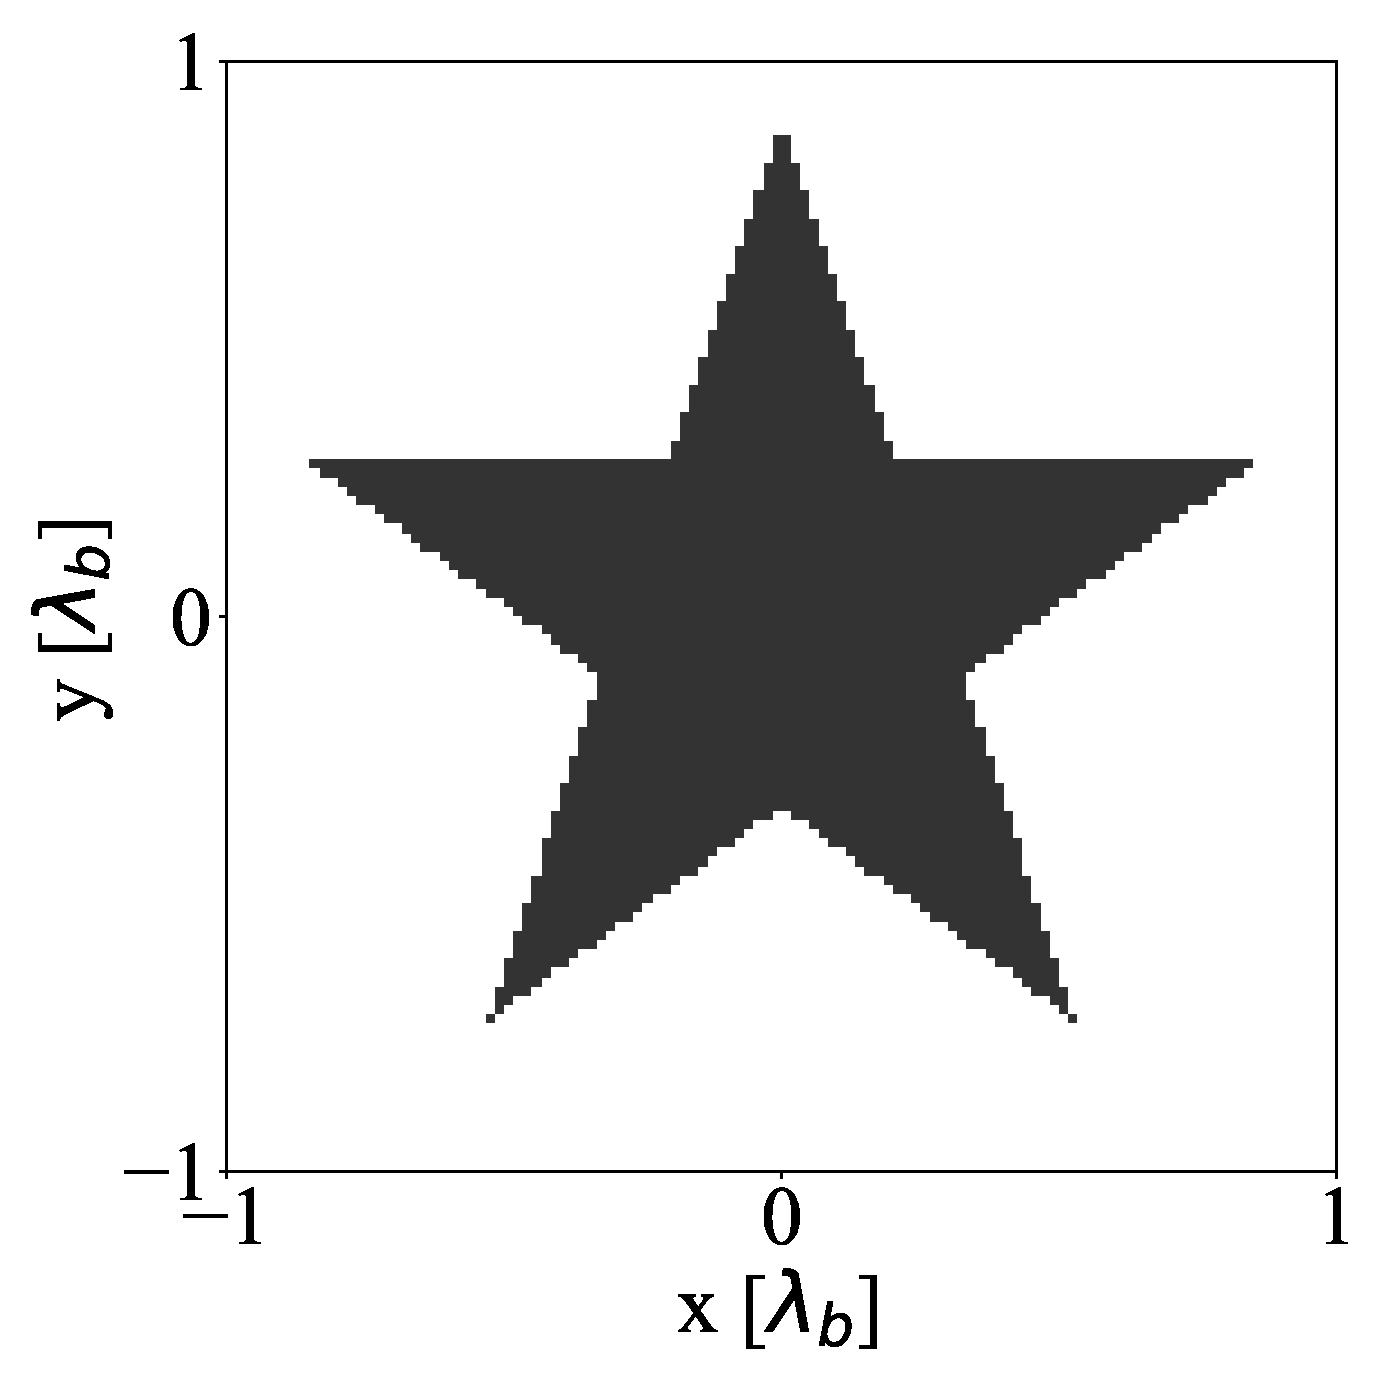
\includegraphics[width=.205\textwidth]{./experiments/indicatorcomparison/shape/figs/groundtruth.eps}\label{fig:shape:indicatorcomparison:groundtruth}}
                \subfigure[SOM: 10 iterations]{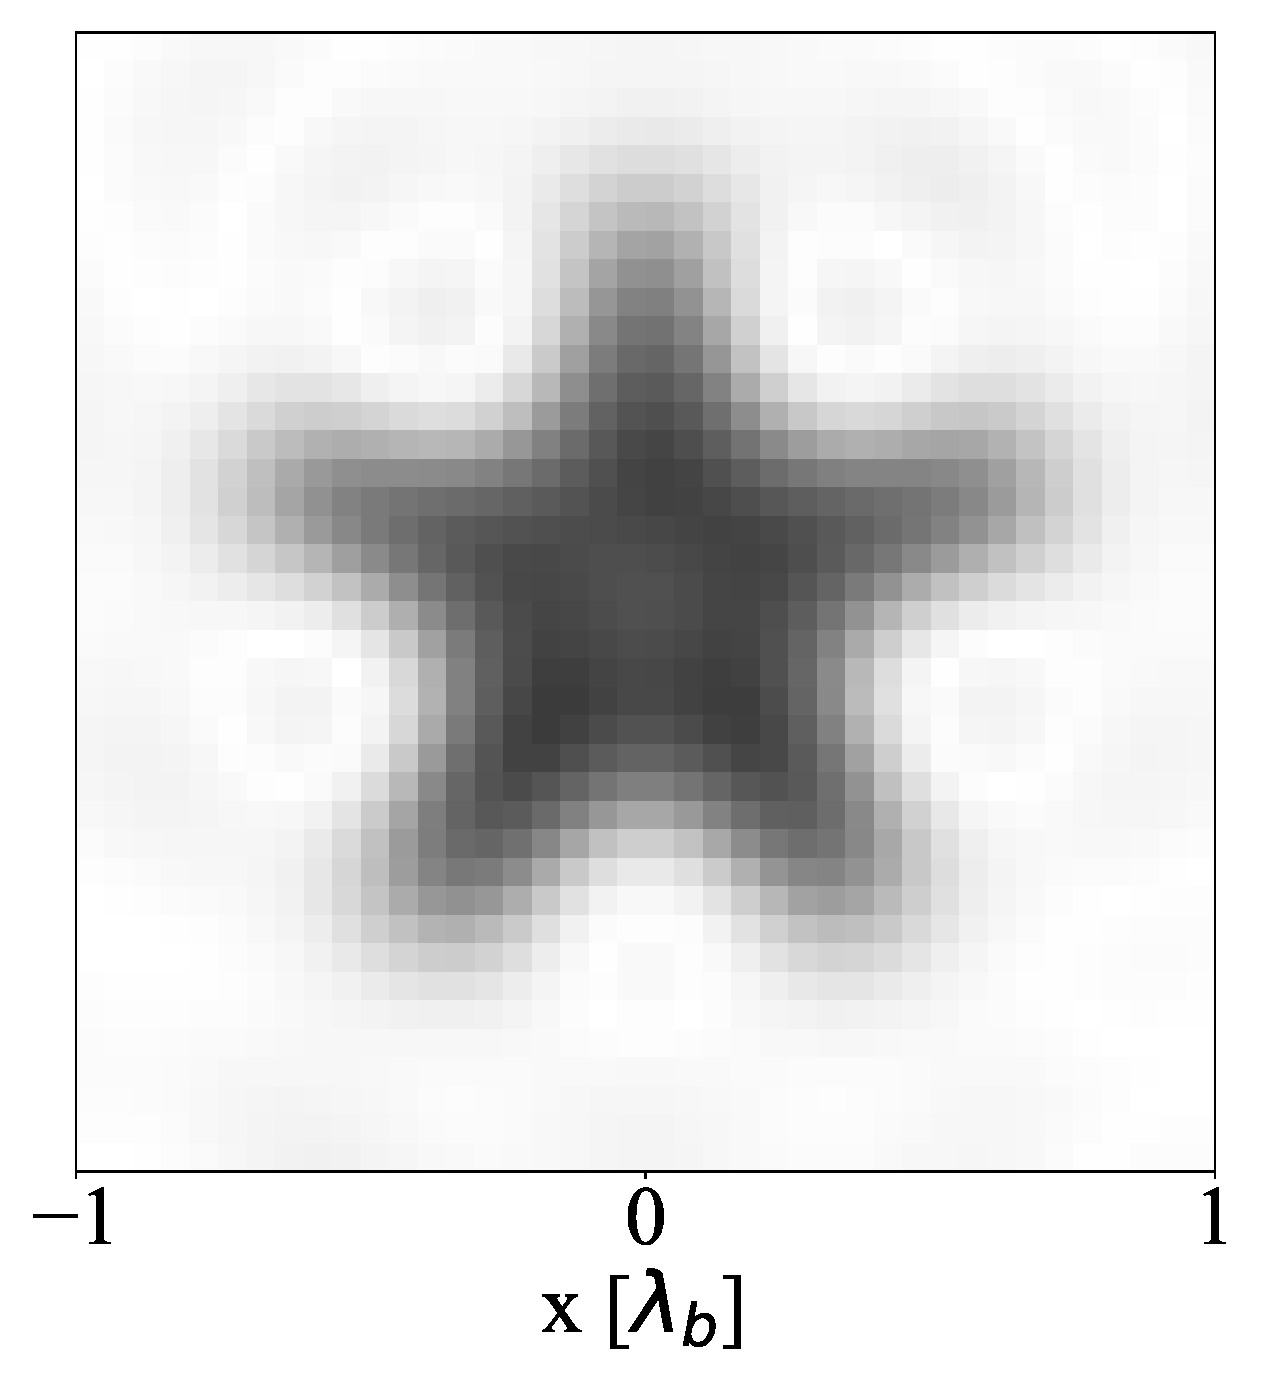
\includegraphics[width=.18\textwidth]{./experiments/indicatorcomparison/shape/figs/som10.eps}\label{fig:shape:indicatorcomparison:som:10}}
                \subfigure[SOM: 20 iterations]{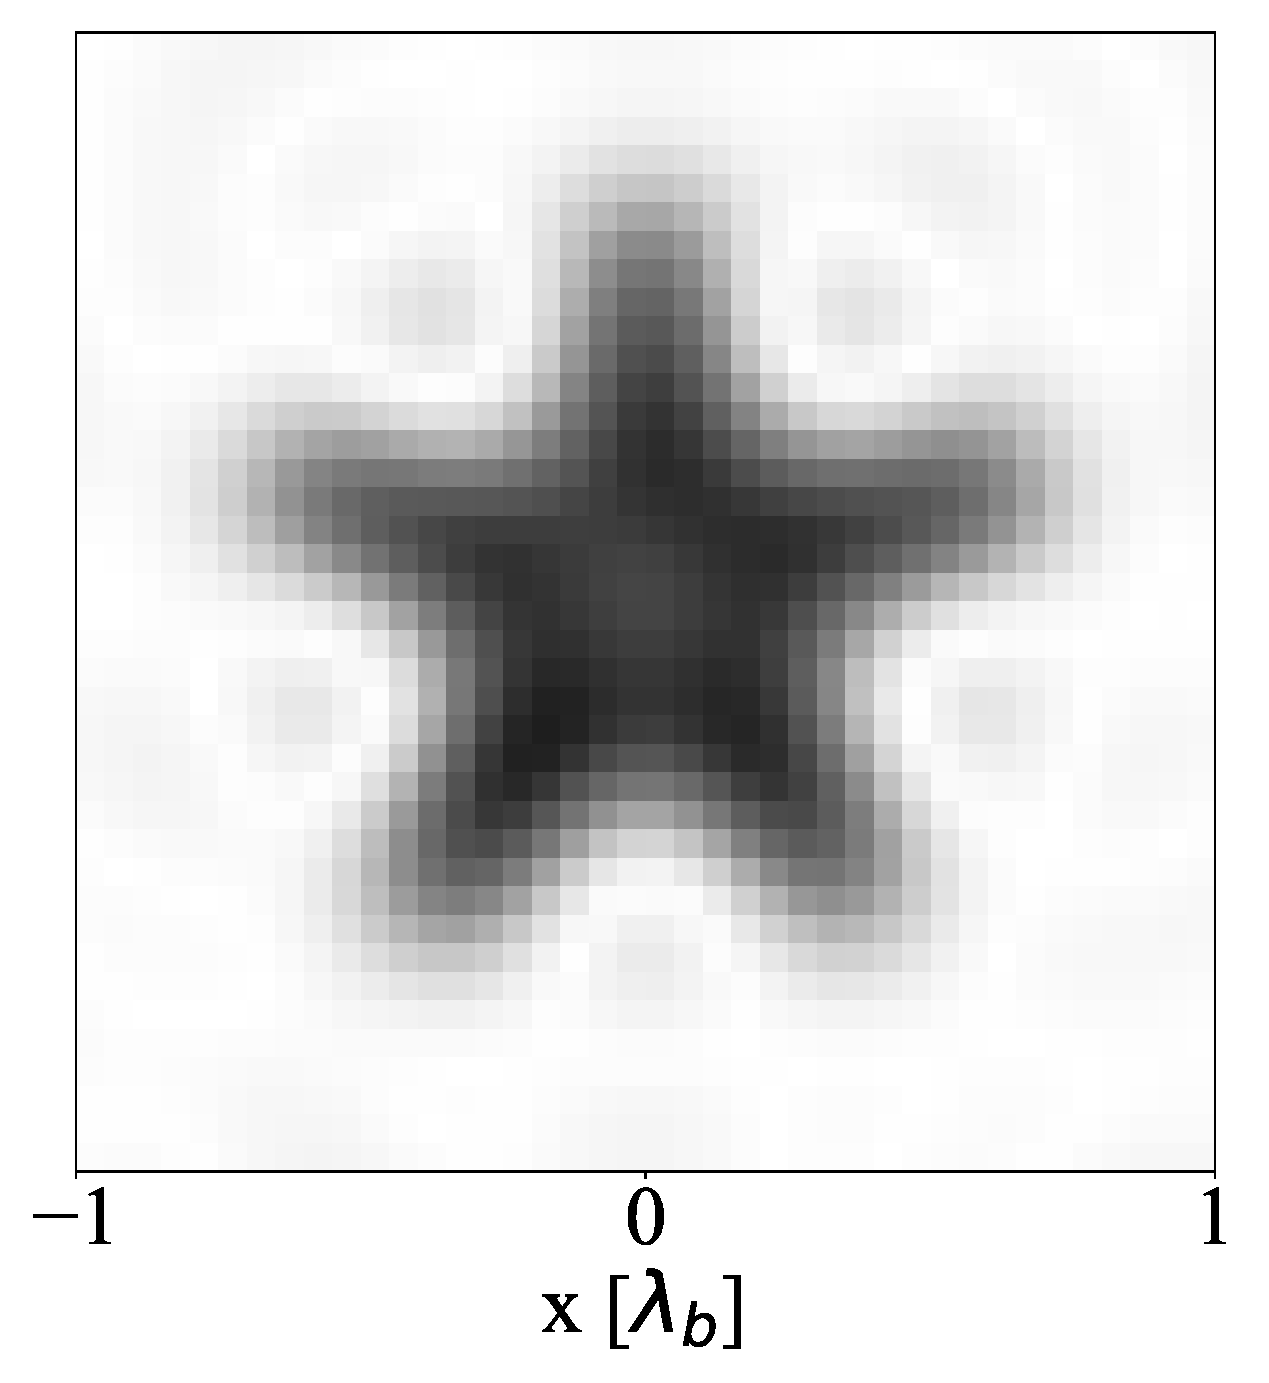
\includegraphics[width=.18\textwidth]{./experiments/indicatorcomparison/shape/figs/som20.eps}\label{fig:shape:indicatorcomparison:som:20}} 
                \subfigure[SOM: 30 iterations]{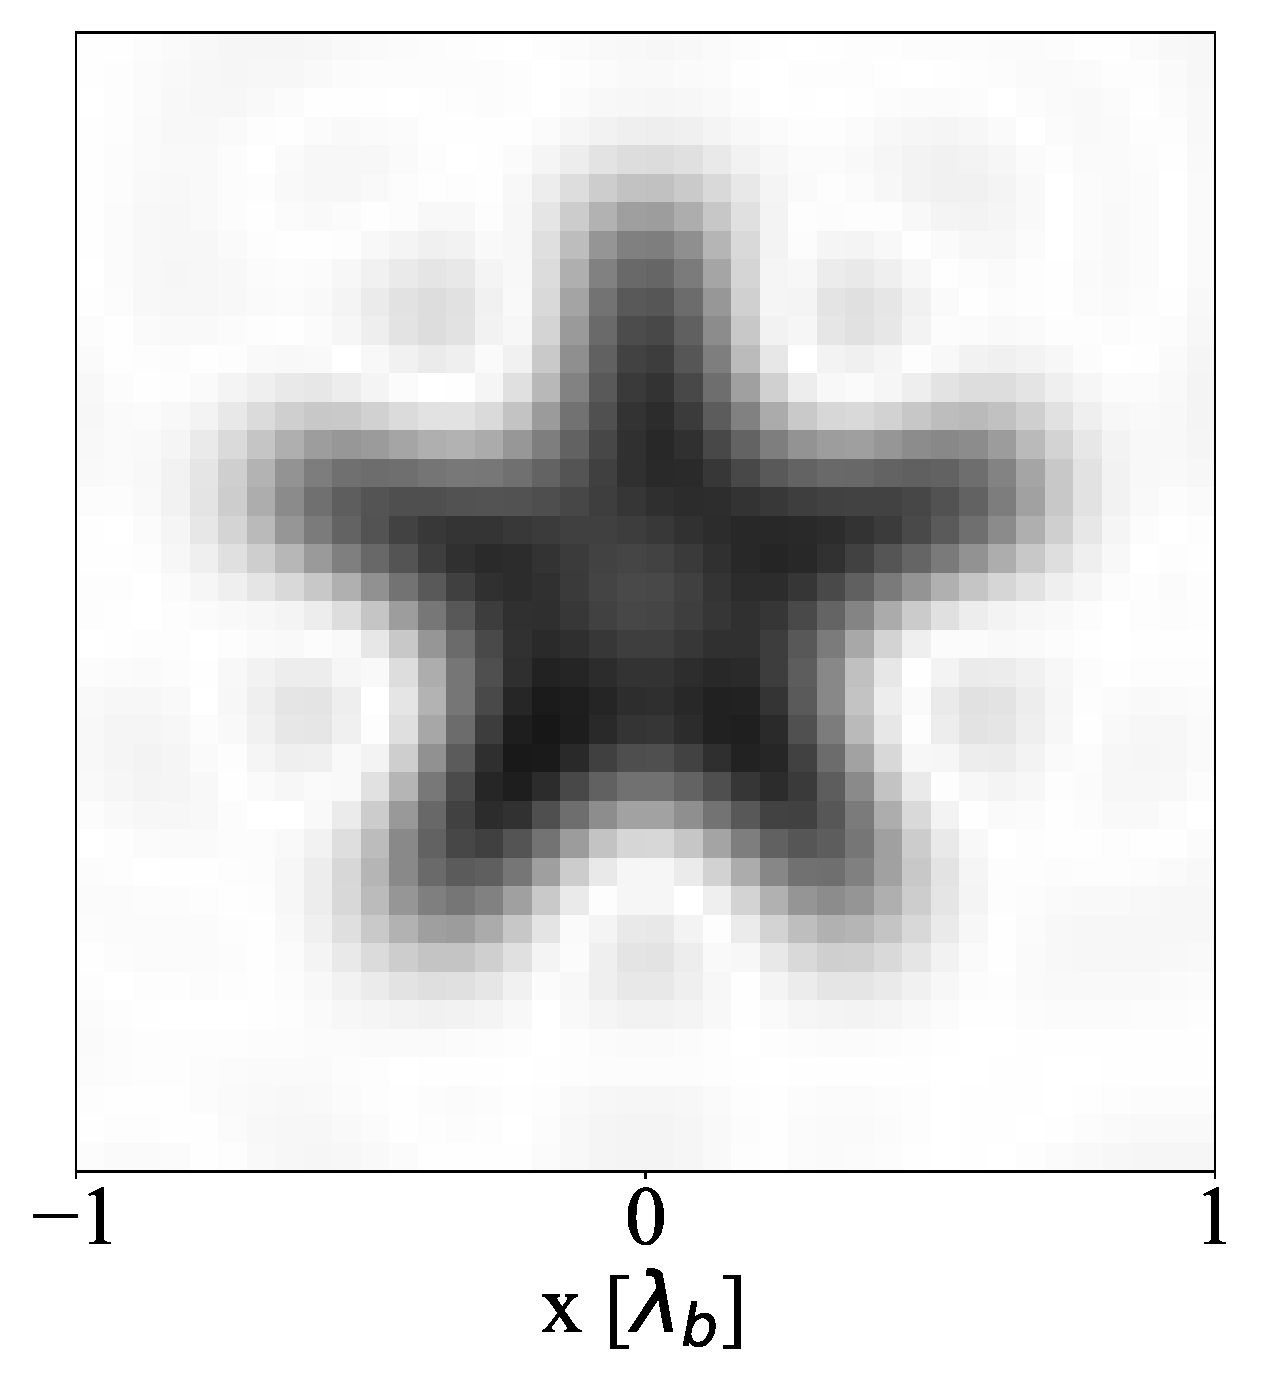
\includegraphics[width=.18\textwidth]{./experiments/indicatorcomparison/shape/figs/som30.eps}\label{fig:shape:indicatorcomparison:som:30}}
                \subfigure[SOM: 100 iterations]{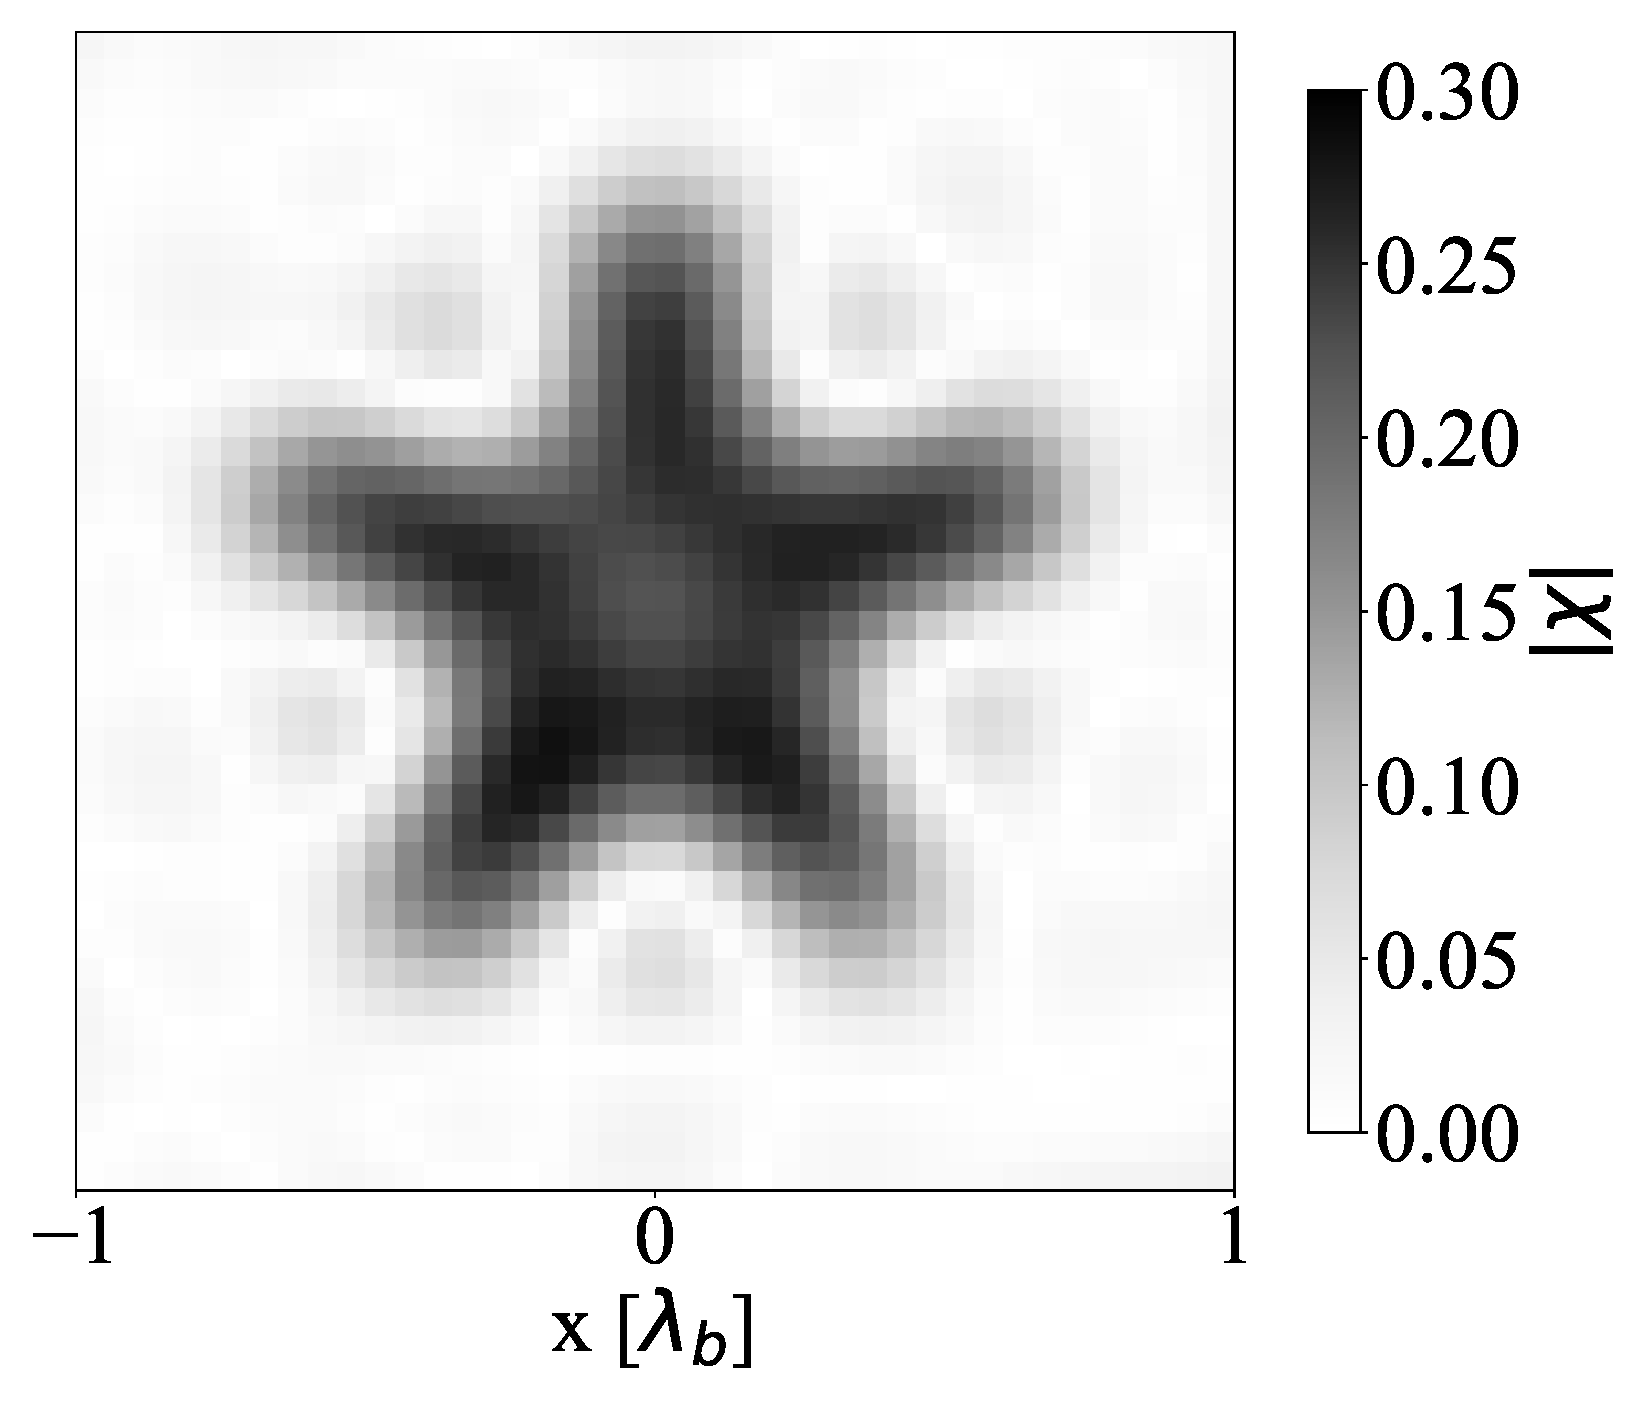
\includegraphics[width=.232\textwidth]{./experiments/indicatorcomparison/shape/figs/som100.eps}\label{fig:shape:indicatorcomparison:som:100}}
                \caption{Shape recovery study, indicator comparison: (a) ground-truth and images recovered by SOM in (b) 10, (c) 20, (d) 30, and (e) 100 iterations.}
                \label{fig:shape:indicatorcomparison:recons}
            \end{figure*}

            Fig. \ref{fig:shape:indicatorcomparison:recons} displays the ground-truth image and the images reconstructed by SOM at iterations 10, 20, 30, and 100. As the number of iterations increases, some observable changes occur in the reconstructed images. The contrast estimation rises slightly with each iteration, with the estimated values remaining moderately above the true contrast value. The star edges become gradually more defined as iterations increase. However, the most significant changes occur in the background medium characteristics. Variations in the vicinity of the star become progressively more pronounced with increasing iterations, while regions farther from the star exhibit a significantly more homogeneous background medium as the iterative process continues.

            \begin{figure}
                \centering
                \subfigure[]{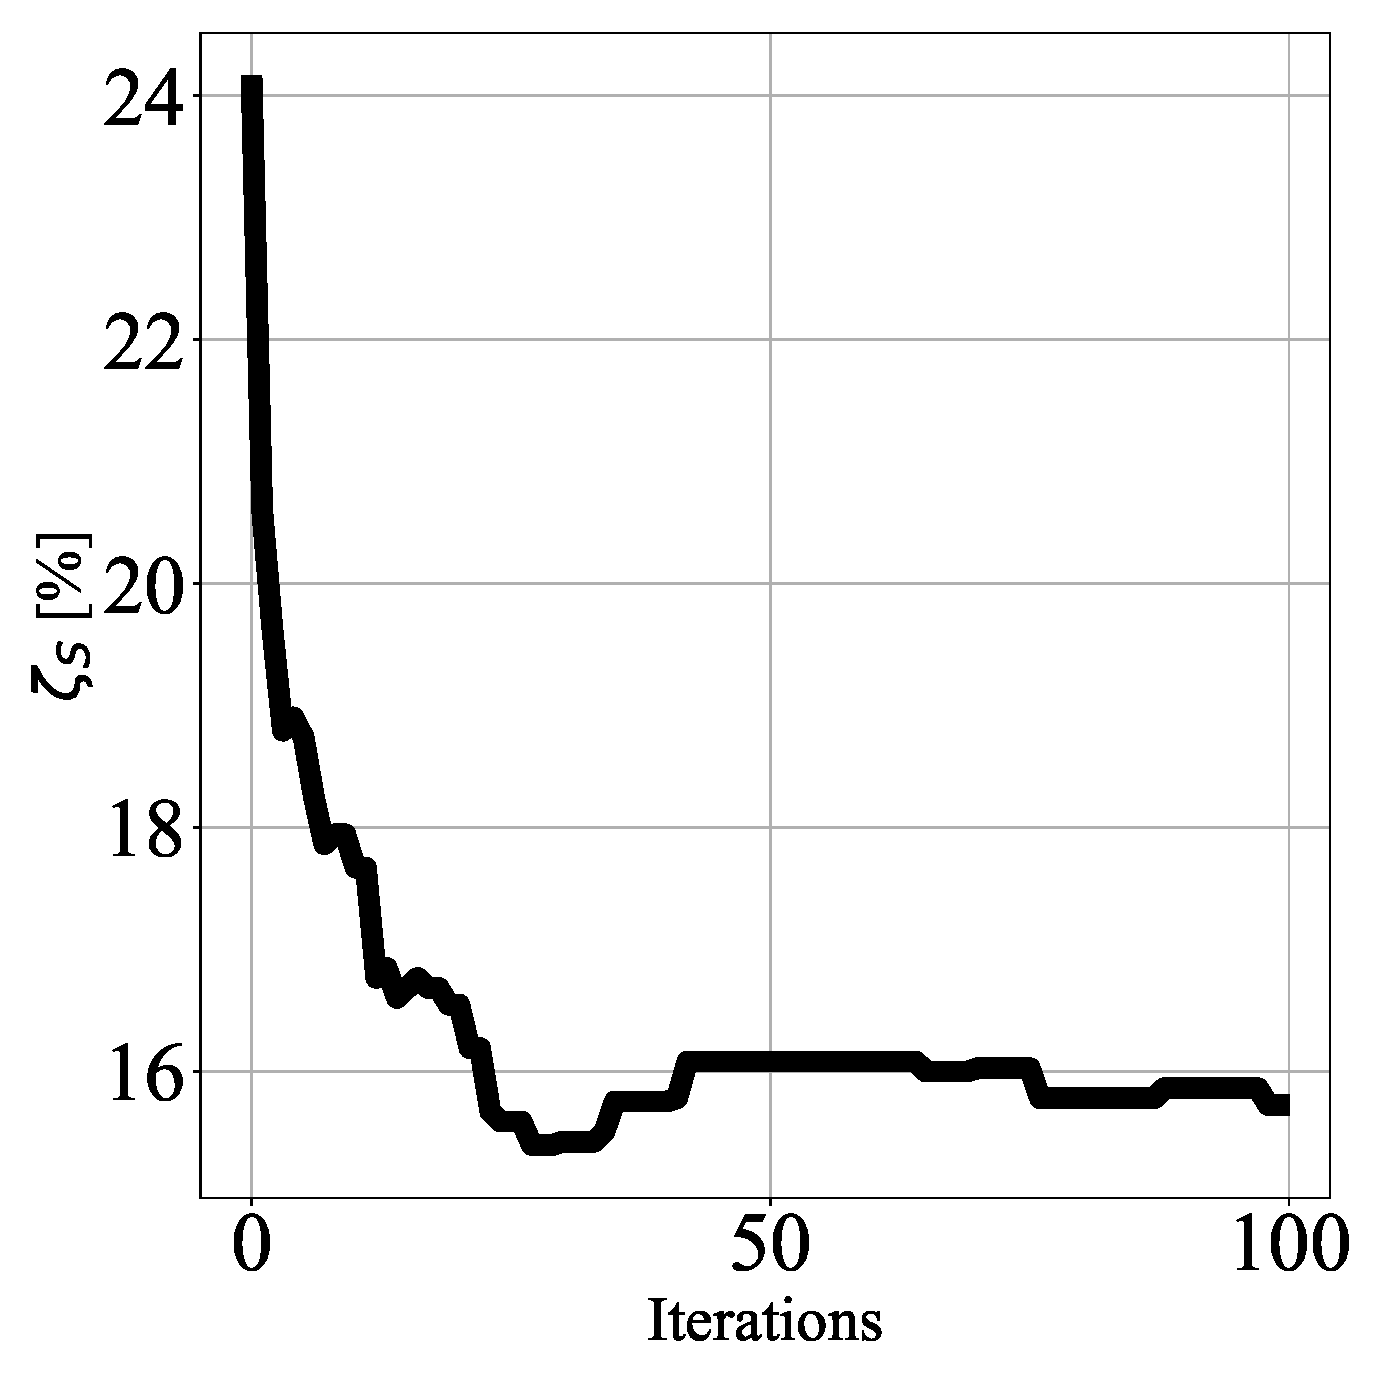
\includegraphics[width=.45\columnwidth]{./experiments/indicatorcomparison/shape/figs/zeta_s.eps}\label{fig:shape:indicatorcomparison:zeta_s}} \hspace{0.05\columnwidth}
                \subfigure[]{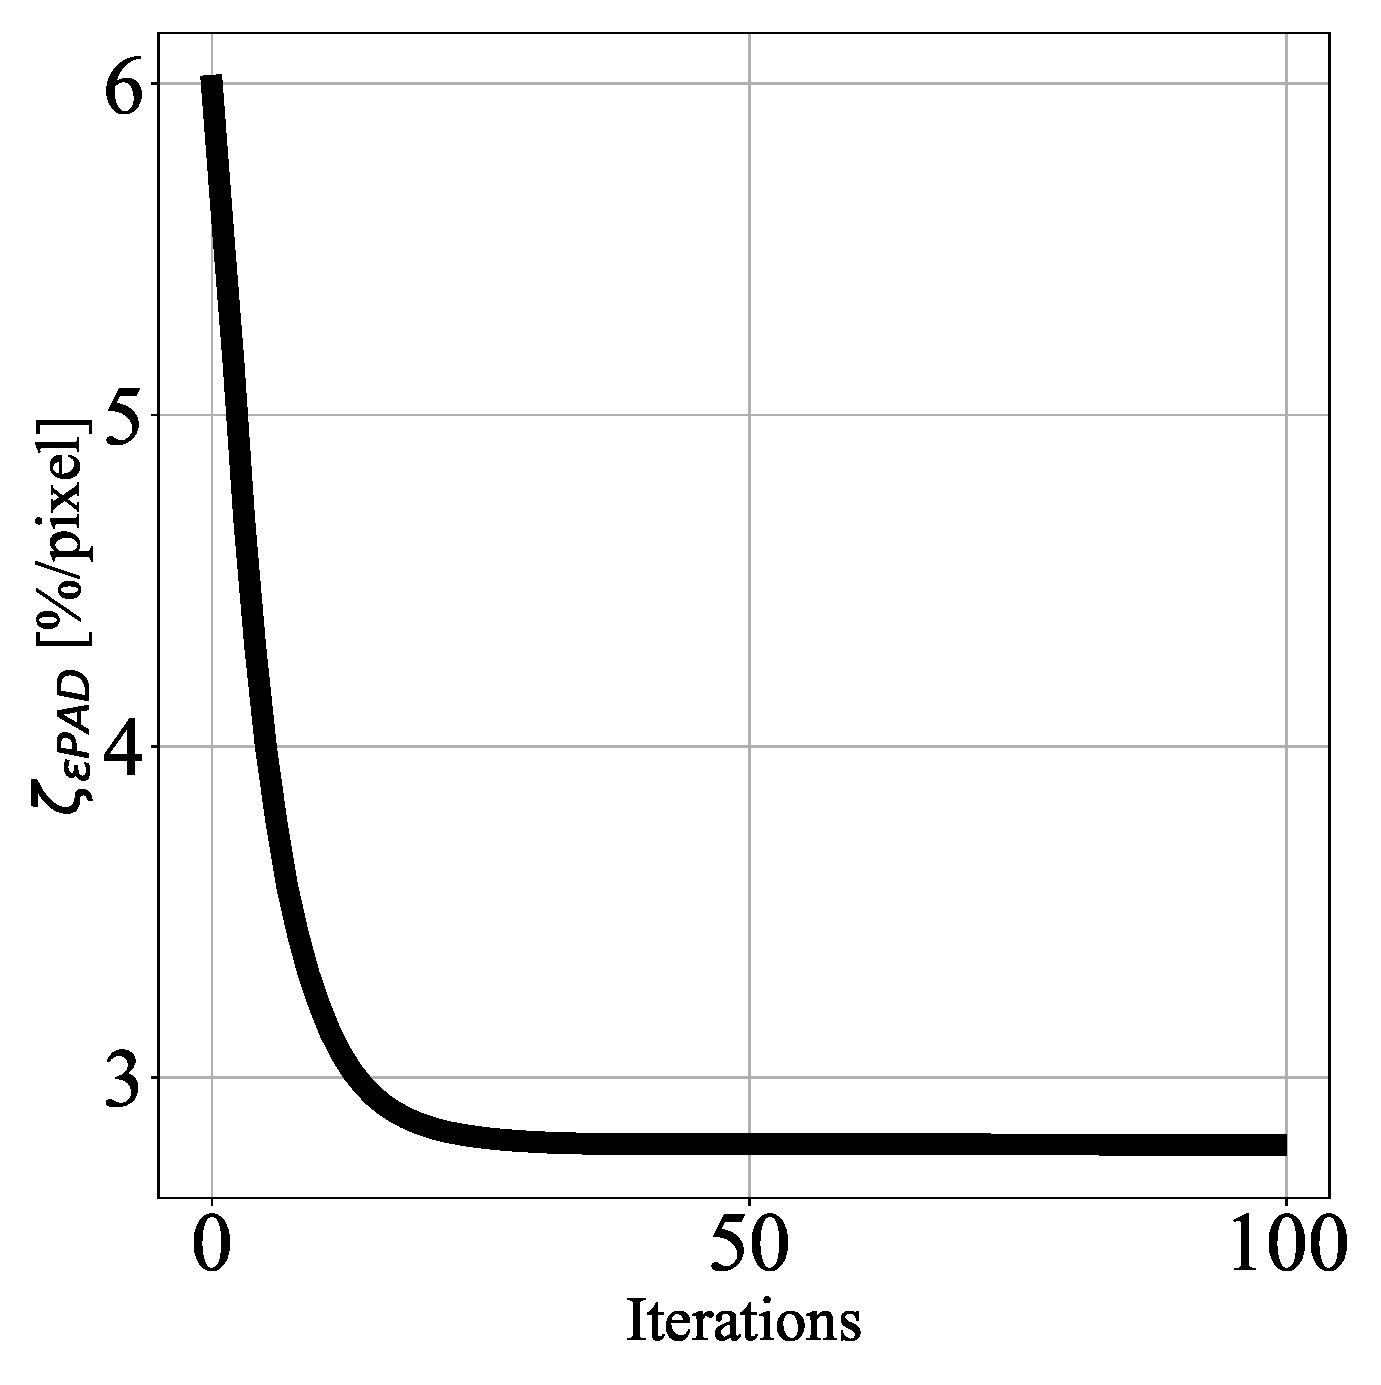
\includegraphics[width=.45\columnwidth]{./experiments/indicatorcomparison/shape/figs/zeta_epad.eps}\label{fig:shape:indicatorcomparison:rmse}} \\
                \subfigure[]{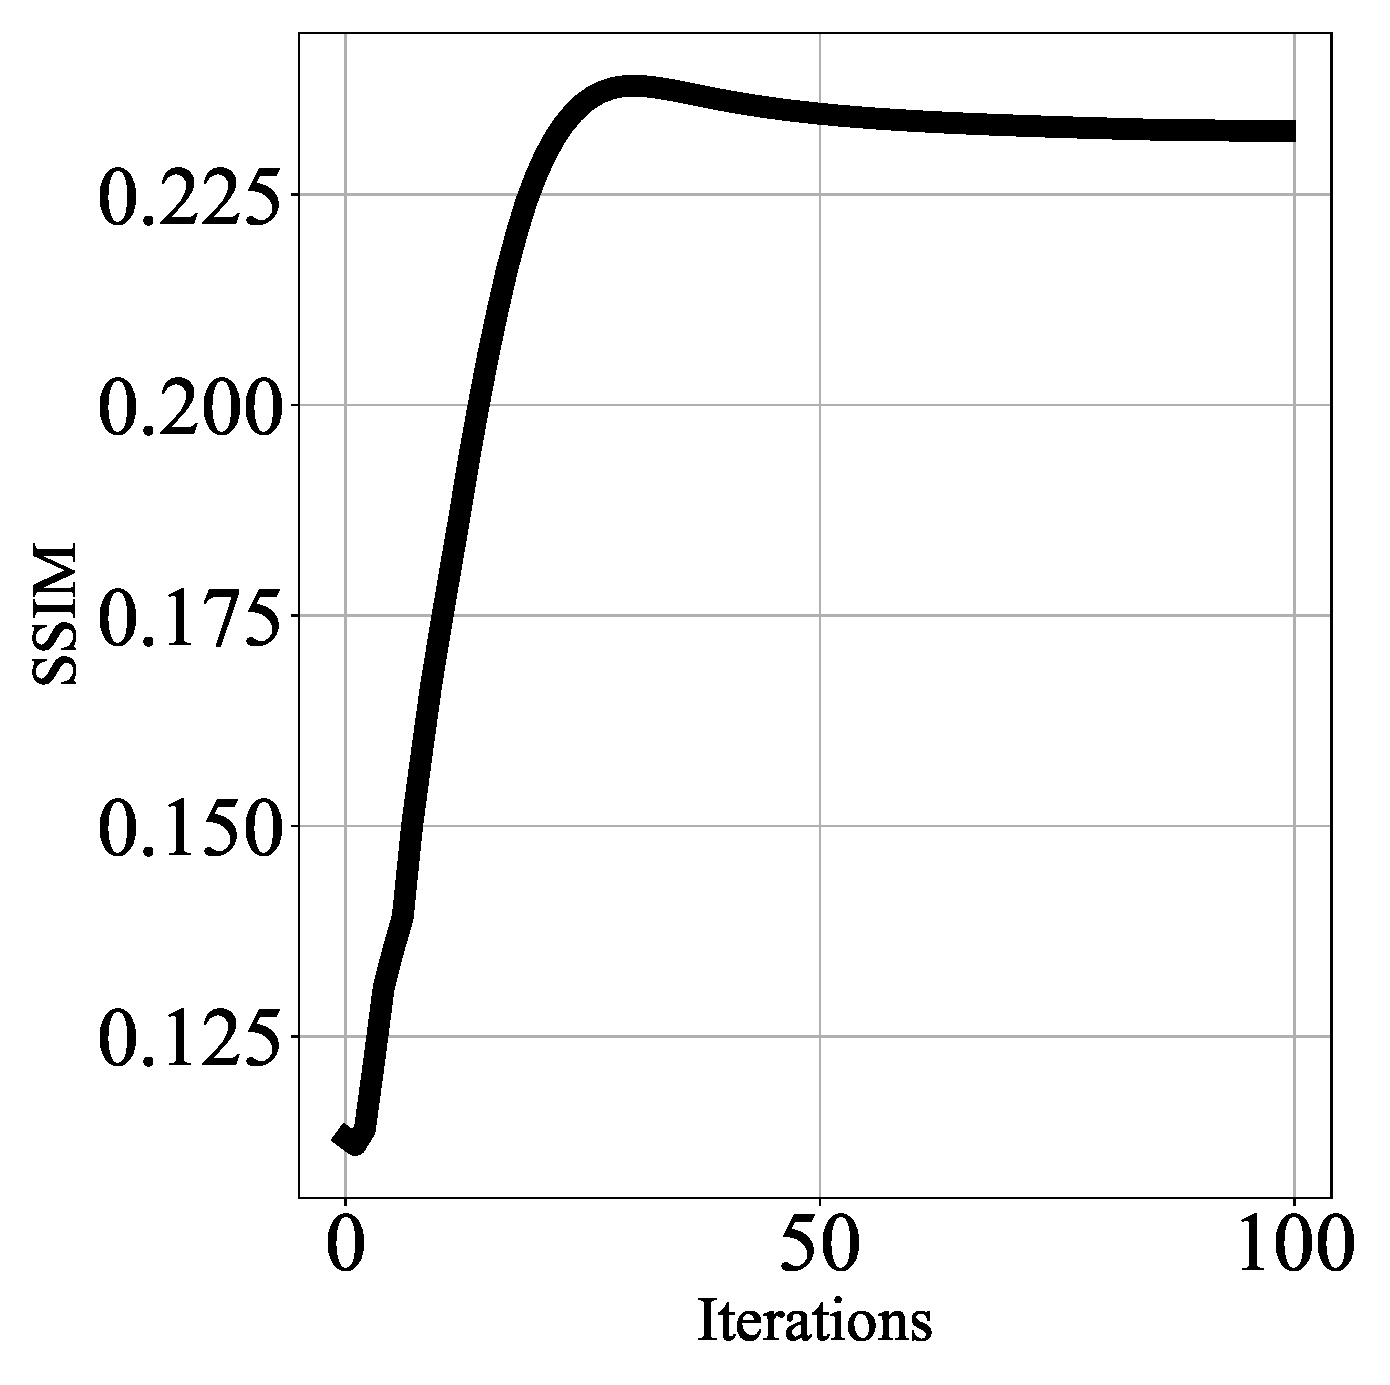
\includegraphics[width=.45\columnwidth]{./experiments/indicatorcomparison/shape/figs/ssim.eps}\label{fig:shape:indicatorcomparison:ssim}}
                \caption{Shape recovery study, indicator comparison: (a) shape error indicator $\zeta_S$, (b) $\zeta_{\epsilon PAD}$ (RMSE), and (c) SSIM for images recovered by SOM in 100 iterations.}
                \label{fig:shape:indicatorcomparison:indicators}
            \end{figure}

            Fig. \ref{fig:shape:indicatorcomparison:indicators} presents the values of the three indicators for the reconstructed images at each iteration. It is important to note that the ideal value of SSIM is 1, indicating identical images, while the ideal values of both $\zeta_S$ and $\zeta_{\epsilon PAD}$ are 0, indicating the absence of error. Consequently, SSIM increases with image quality improvement, whereas the other two indicators decrease. The results reveal a tendency toward stability in the indicator values starting from iteration 30 or 50. Notably, the SSIM value remains considerably distant from 1. Furthermore, both $\zeta_S$ and $\zeta_{\epsilon PAD}$ exhibit smooth variations throughout the iterative process. However, $\zeta_S$ displays small irregularities in the decay, which can be attributed to the discrete nature of the thresholding operation inherent to its calculation methodology.

            The distance of the SSIM indicator from the ideal level (1) can be explained by the influence that background medium variations exert on the indicator calculation. This also occurs in the RMSE ($\zeta_{\epsilon PAD}$) calculation, although the impact is less pronounced due to the way the error is computed. On the other hand, the $\zeta_S$ indicator is less affected by these background medium variations, since the thresholding process tends to eliminate these small fluctuations, focusing primarily on the recovery of the scatterer geometry. This represents an advantage of the proposed indicator, especially in scenarios where accurate recovery of the scatterer geometry is the primary objective.

    \subsection{Position Detection Study}\label{sec:results:position}

        In many scenarios where algorithms can adequately reconstruct the geometry of scatterers, the error in detecting scatterer positions tends to be low. For example, in the study described in Section \ref{sec:results:shape:star}, the $\zeta_P$ indicator values obtained by LSM, OSM, BIM, CSI, and SOM were 0.049\%, 0.057\%, 0.25\%, 0.31\%, and 0.14\%, respectively. This occurs because geometry and position are scatterer characteristics that algorithms typically do not handle separately.

        An exception would be algorithms that solve the imaging problem as an optimization problem, where the decision variables are the position, vertices (or other characteristics of a predefined geometry), and contrast of the scatterers \cite{michalski2000electromagnetic,salucci2022learned,zardi2025physics}. Additionally, in scenarios involving strong scatterers with small size compared to the wavelength, traditional methods generally struggle to recover scatterer geometry effectively due to the increased problem hardness. In such scenarios, studying position detection becomes more relevant.

        Considering this, the experiments in this section were designed for scenarios involving strong scatterers with small dimensions, where traditional methods cannot adequately recover scatterer geometry. Therefore, the position error indicator $\zeta_P$ serves as a relevant metric for comparing algorithm performance in such challenging scenarios. In addition, the DOI discretization for data synthesis was performed using a finer grid with $160 \times 160$ pixels.

        For all subsequent experiments, LSM was removed and an other method was introduced. Since the analytical solution for scattering from an infinite dielectric cylinder is well-established \cite{harrington2001time}, it becomes possible to determine the optimal circular approximation (defined by radius, $x$-$y$ center position, and contrast) that best fits the scattered field of any single scatterer.

        To optimize these four parameters, we employ a two-stage approach \cite{virtanen2020SciPy}:
        \begin{enumerate}
            \item Global optimization: The Differential Evolution (DE) algorithm \cite{storn1997differential} with 50 generations, 15 individuals, crossover rate of 0.7, and mutation factor ranging from 0.5 to 1.
            \item Local refinement: The L-BFGS-B algorithm \cite{zhu1997algorithm} for improved accuracy.
        \end{enumerate}

        While DE is inherently stochastic and would typically require multiple executions for robust analysis, the problem structure and subsequent refinement step allow for single execution per instance based on previous experimental validation. This methodology is referred to as Circle Approximation (CA) throughout this work.

        It should be noted that \cite{michalski2000electromagnetic} employed a similar DE-based approach for circular fitting, though their work focused specifically on perfect electric conductor cylinders under cylindrical scatterer assumptions.

        \subsubsection{Single scatter}\label{sec:results:position:single}

            The first scenario for studying the position indicator utilized a star-shaped scatterer, similar to the experiments described in Sections \ref{sec:results:shape:star} and \ref{sec:results:shape:varying}. However, this configuration featured the scatterer positioned in the upper-right corner and rotated by 30 degrees, as illustrated in Fig. \ref{fig:position:single:ground_truth}. The scatterer contrast was set to 7, while the radius from the center to the farthest vertices was reduced to 0.15$\lambda_b$. Under these configurations, the DNL for this experiment reaches 1.7, which is slightly above the threshold of 1.

            Fig. \ref{fig:position:single:recons} shows the images reconstructed by each algorithm. As expected, given the high contrast and small scatterer size, the methods reconstruct small blobs in the scatterer region. The way these blobs are reconstructed is relevant, as this information directly impacts the measurement of scatterer position. 

            In this regard, CSI experienced the greatest reconstruction difficulty, with contrast concentrated in a very small region and significantly lower contrast levels compared to the other quantitative methods. It is also notable that CA most closely approximated the actual scatterer contrast.

            \begin{figure*}[!htb]
                \centering
                \subfigure[Ground-Truth]{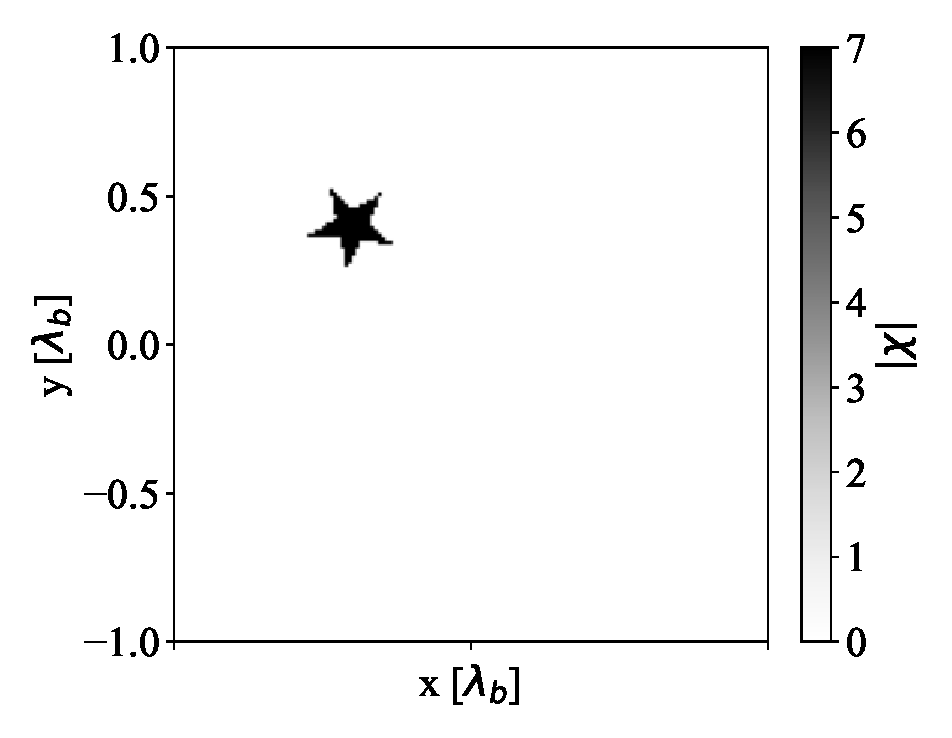
\includegraphics[height=0.5\columnwidth]{../experiments/position/single/figs/0.eps}\label{fig:position:single:ground_truth}}
                \subfigure[OSM]{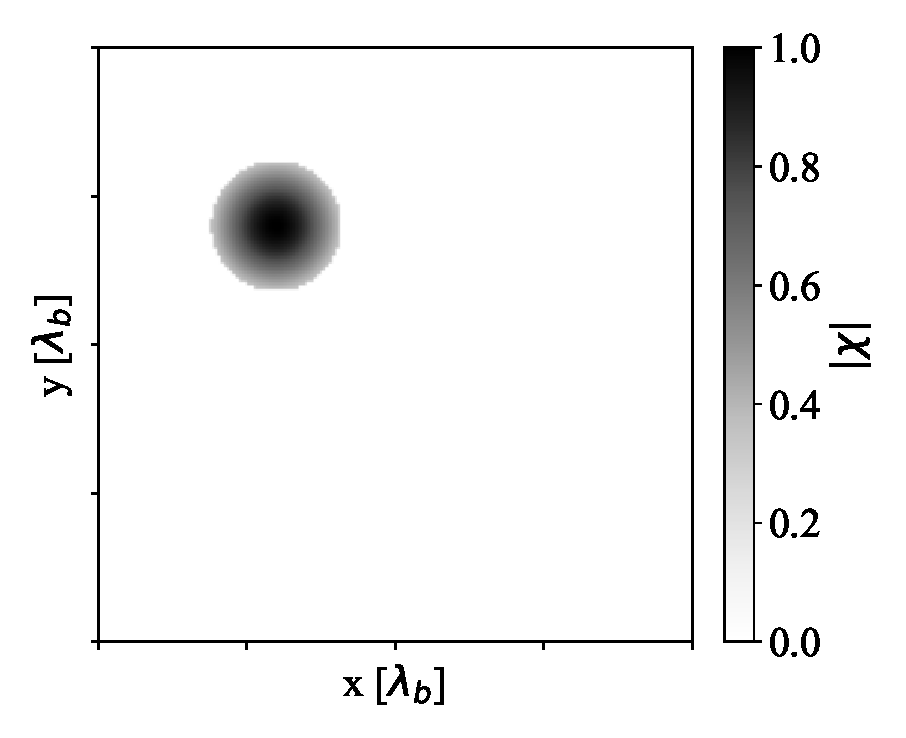
\includegraphics[height=0.5\columnwidth]{../experiments/position/single/figs/1.eps}}
                \subfigure[BIM]{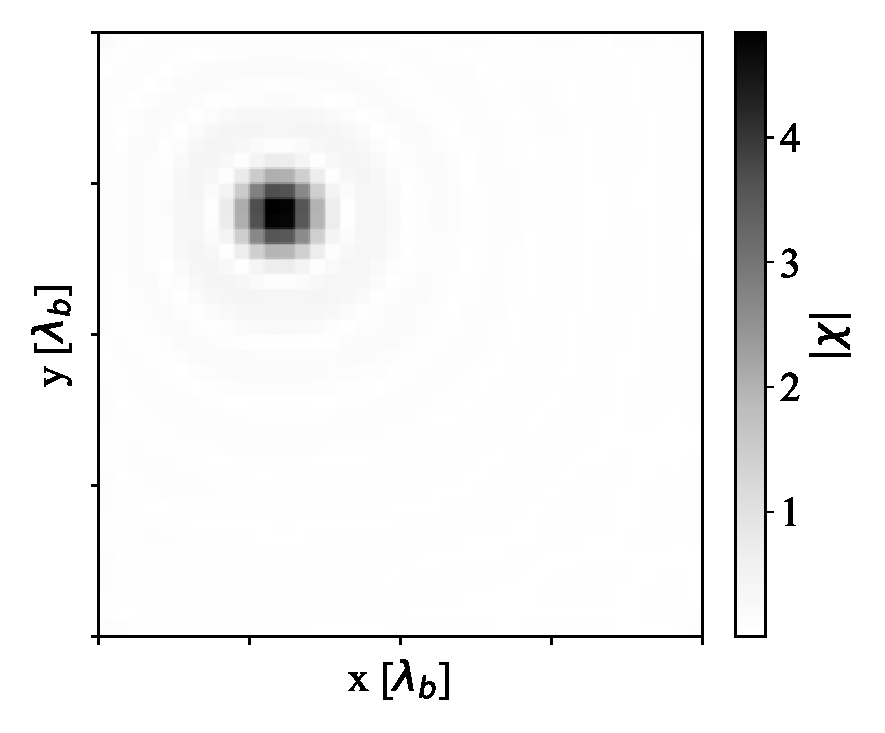
\includegraphics[height=0.5\columnwidth]{../experiments/position/single/figs/2.eps}} \\
                \subfigure[CSI]{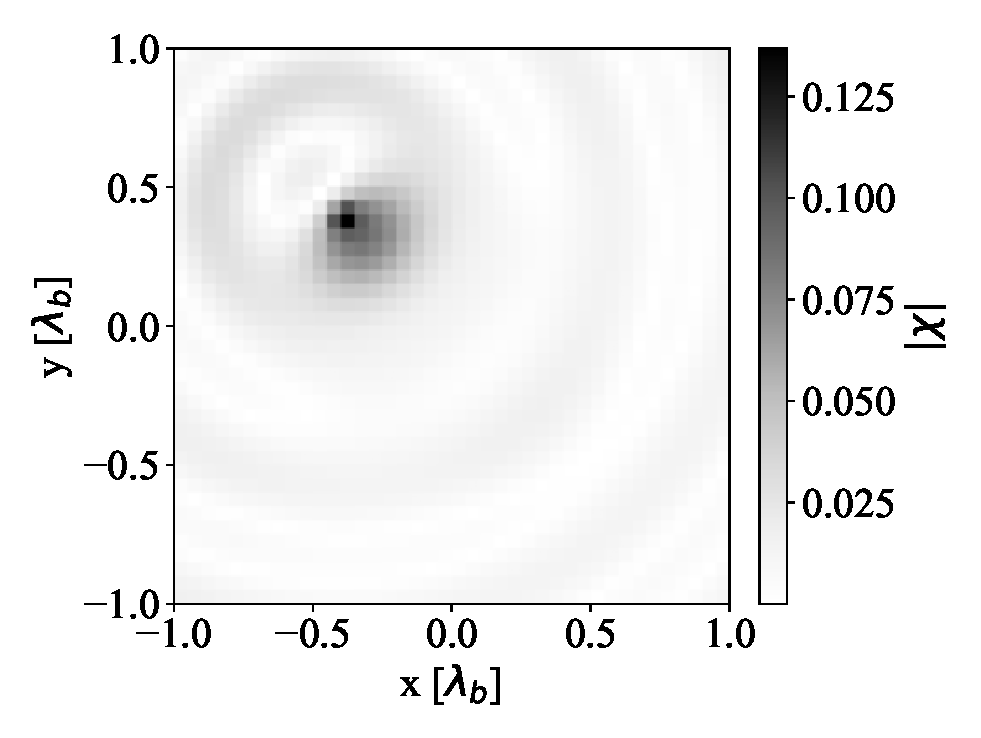
\includegraphics[height=0.5\columnwidth]{../experiments/position/single/figs/3.eps}}
                \subfigure[SOM]{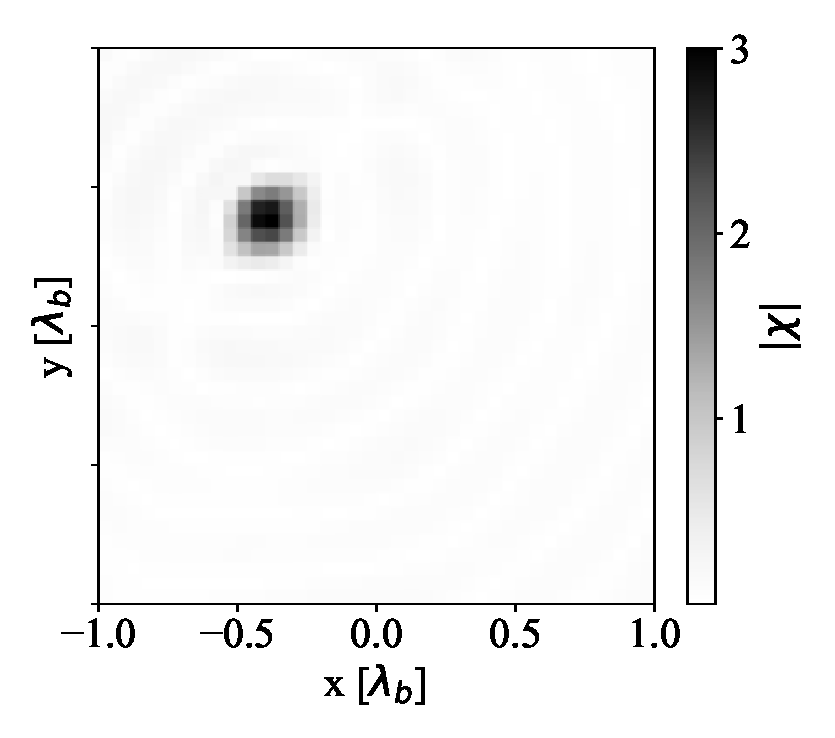
\includegraphics[height=0.5\columnwidth]{../experiments/position/single/figs/4.eps}}
                \subfigure[CA]{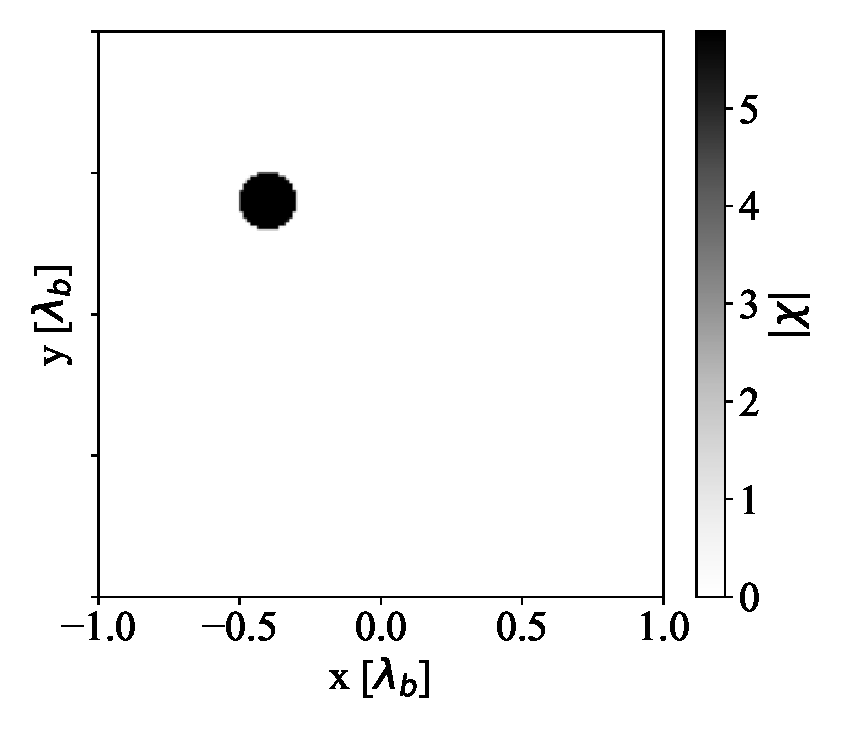
\includegraphics[height=0.5\columnwidth]{../experiments/position/single/figs/5.eps}}
                \caption{Position detection study, single scatterer: ground-truth and reconstructed images by each algorithm.}
                \label{fig:position:single:recons}
            \end{figure*}

            Table \ref{tab:position:single:zeta_p} summarizes the results of the position error indicator for each algorithm. The results indicate that OSM, BIM, and CA achieved the best performance, while SOM performed similarly. The largest error was observed for CSI, which, due to its greater difficulty in quantifying the object's contrast, had more difficulty in capturing the object's position. Generally, the position detection errors for most algorithms were low. However, there may be applications where precision in position detection is critical, such as in tumor detection, for example.

            \begin{table}[!htb]
                \centering
                \renewcommand{\arraystretch}{1.5}
                \caption{Position detection study, single scatterer: position error indicator $\zeta_P$ for each algorithm.}
                \label{tab:position:single:zeta_p}
                \begin{tabular}{cccccc}
                    Method & OSM & BIM & CSI & SOM & CA \\\hline
                    $\zeta_P$ (\%) & 0.08 & 0.04 & 4.68 & 0.53 & 0.04 \\
                \end{tabular}   
            \end{table}
        
        \subsubsection{Multiple scatterers}\label{sec:results:position:multiple}

            Although the proposed indicator for measuring position error was designed for scenarios with a single scatterer, it can also be applied in scenarios with multiple scatterers. In these cases, the centroid of the arrangement as a whole serves as the reference point for measuring position error. This type of investigation can be useful for applications such as through-wall imaging, for example.

            Based on this approach, this experiment considers three scatterers: the star from the previous experiment, a square, and a cross. The contrasts of the three scatterers were set to 4, 3.5, and 2.5, respectively. These values were chosen to be lower than in the previous experiment, since the presence of multiple scatterers inherently increases problem hardness due to mutual current induction between the scatterers.

            The square has a side length of 0.15$\lambda_b$, while the cross has dimensions of 0.3$\lambda_b$ × 0.3$\lambda_b$ with a thickness of 0.15$\lambda_b$. The scatterers were positioned such that their collective arrangement is located in the upper corner of the DOI, as illustrated in Fig. \ref{fig:position:multiple:ground_truth}. Under this configuration, the DNL for this experiment is 0.3.

            Fig. \ref{fig:position:multiple:recons} presents the reconstructions obtained by each algorithm for the multiple scatterer scenario. As expected in this small-size configuration, the algorithms produce blob-like structures that are generally larger than the actual object geometries. The CA method positioned its circular approximation close to the square's location. Although the quantitative methods could not accurately estimate the individual scatterer contrasts, they consistently assigned higher contrast values to the square region rather than the star region. This behavior suggests that the square's larger cross-sectional area compared to the star may have influenced the algorithms' reconstruction process.

            \begin{figure*}[!htb]
                \centering
                \subfigure[Ground-Truth]{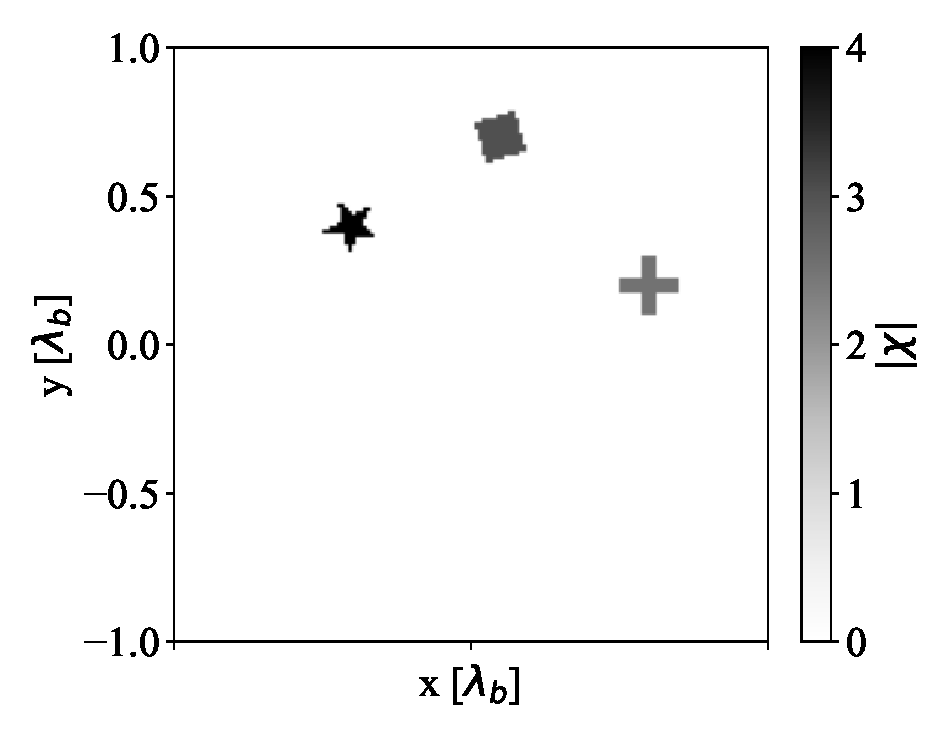
\includegraphics[height=0.5\columnwidth]{../experiments/position/multiple/figs/0.eps}\label{fig:position:multiple:ground_truth}}
                \subfigure[OSM]{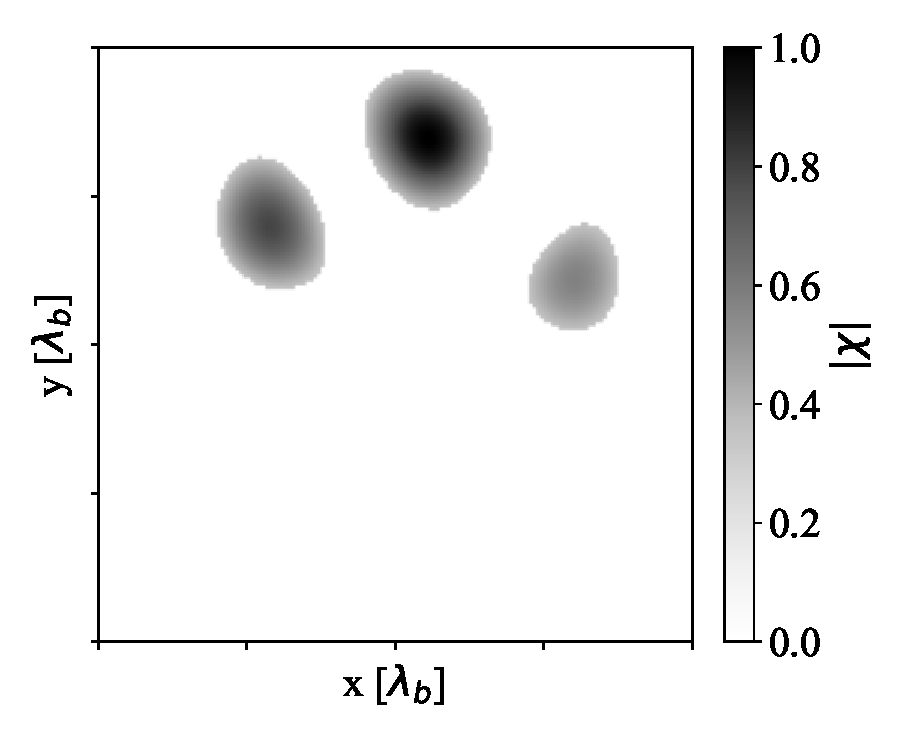
\includegraphics[height=0.5\columnwidth]{../experiments/position/multiple/figs/1.eps}}
                \subfigure[BIM]{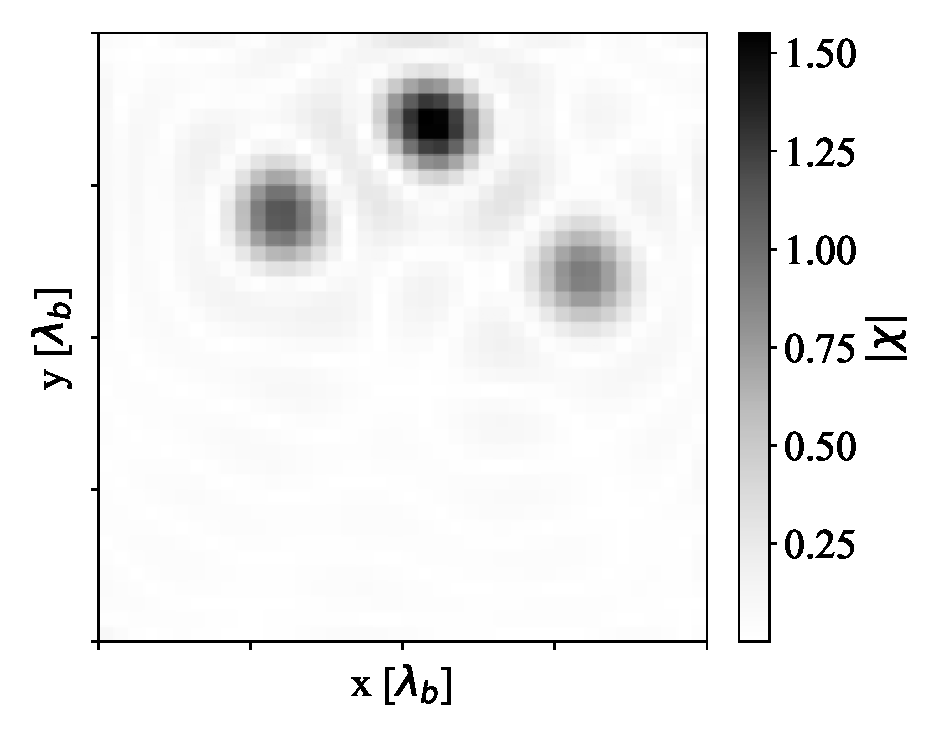
\includegraphics[height=0.5\columnwidth]{../experiments/position/multiple/figs/2.eps}} \\
                \subfigure[CSI]{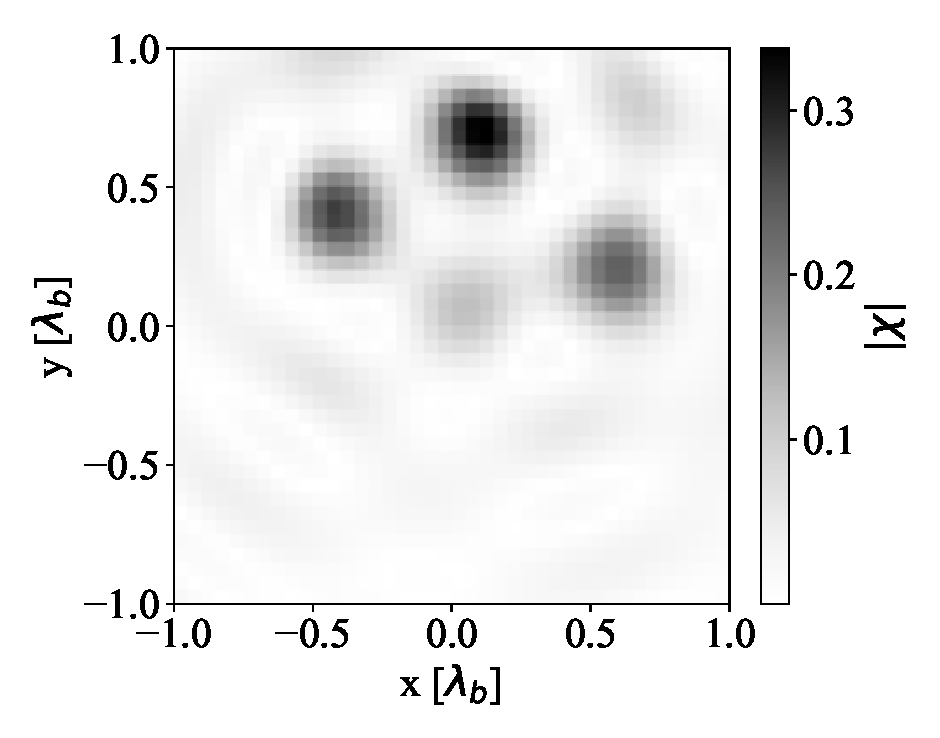
\includegraphics[height=0.5\columnwidth]{../experiments/position/multiple/figs/3.eps}}
                \subfigure[SOM]{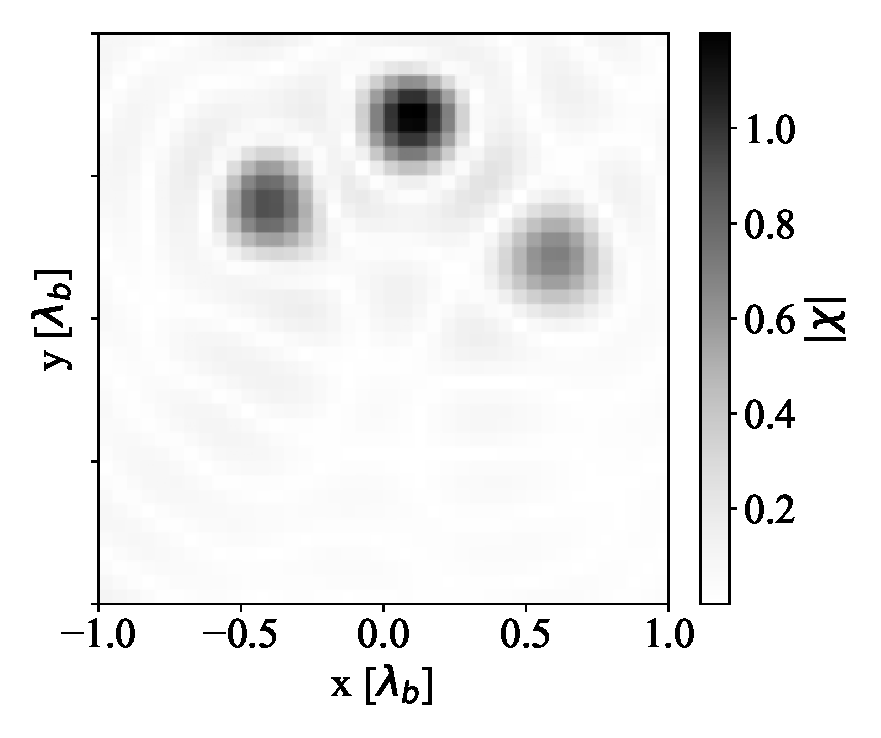
\includegraphics[height=0.5\columnwidth]{../experiments/position/multiple/figs/4.eps}}
                \subfigure[CA]{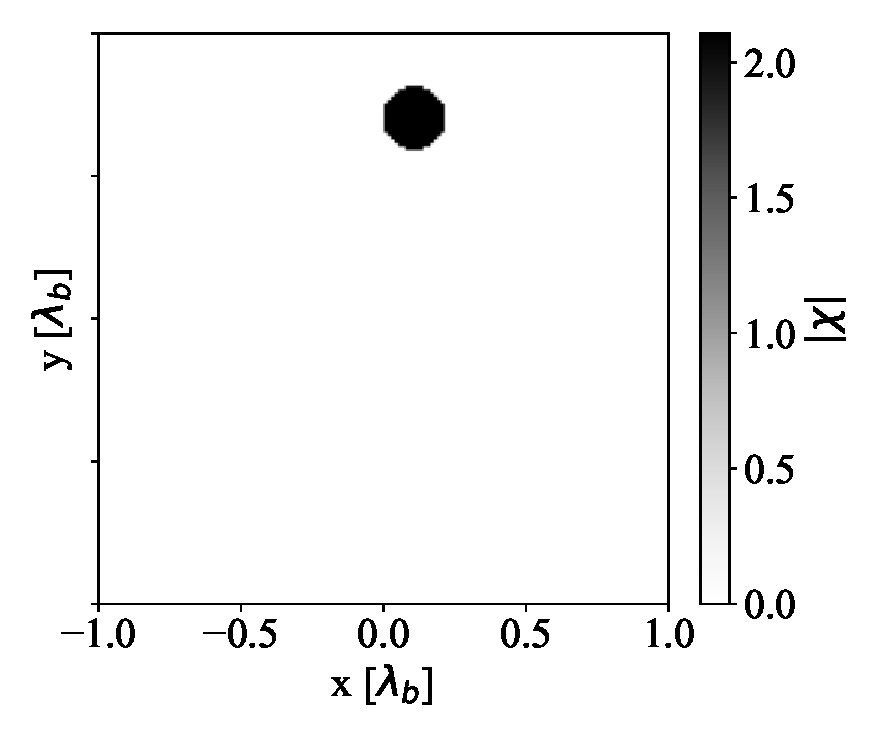
\includegraphics[height=0.5\columnwidth]{../experiments/position/multiple/figs/5.eps}}
                \caption{Position detection study, multiple scatterer: ground-truth and reconstructed images by each algorithm.}
                \label{fig:position:multiple:recons}
            \end{figure*}

            Table \ref{tab:position:multiple:zeta_p} presents the position error results for each algorithm. Interestingly, CSI achieved the best performance in this multi-scatterer scenario, despite its poor performance in the single scatterer case. This suggests that the algorithm's behavior may be different when dealing with multiple targets. BIM and SOM showed similar intermediate performance, while OSM and CA exhibited higher position errors, indicating greater difficulty in accurately localizing the overall scatterer arrangement.

            \begin{table}[!htb]
                \centering
                \renewcommand{\arraystretch}{1.5}
                \caption{Position detection study, multiple scatterers: position error indicator $\zeta_P$ for each algorithm.}
                \label{tab:position:multiple:zeta_p}
                \begin{tabular}{cccccc}
                    Method & OSM & BIM & CSI & SOM & CA \\\hline
                    $\zeta_P$ (\%) & 10.24 & 8.30 & 4.86 & 8.27 & 12.85 \\
                \end{tabular}   
            \end{table}
            
        \subsubsection{Average performance}\label{sec:results:position:benchmark}

            Similar to the shape recovery study, an average performance analysis was conducted to compare the position detection capabilities of OSM, BIM, CSI, SOM, and CA algorithms. This experiment employed 30 scatterer instances with configurations similar to those described in Section \ref{sec:results:position:single}. The scatterer contrast was fixed at 7, and the radius from the center to the farthest vertices was set to 0.15$\lambda_b$. Following the approach from Section \ref{sec:results:shape:average}, the scatterers were randomly generated as polygons with 4 to 15 vertices.

            The DNL distribution is shown in Fig. \ref{fig:position:average:dnl}. The values range from below 1 to above 4, with a median close to 2. The high contrast level and geometric variations contributed to the wide distribution of DNL values. However, as shown in Fig. \ref{fig:position:average:zeta_s}, the algorithm performance within each instance remained within a similar range. CSI clearly exhibited the worst performance, followed by SOM. The best performance in each instance varied between OSM and CA. These results are coherent with the findings from Section \ref{sec:results:position:single}.

            \begin{figure}[!htb]
                \centering
                \subfigure[]{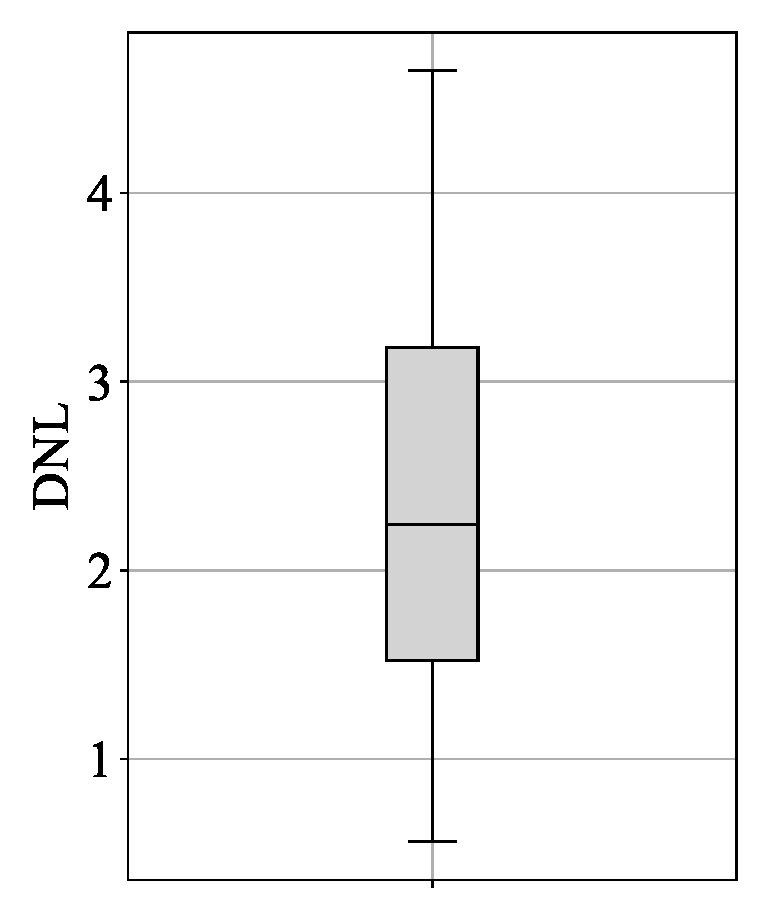
\includegraphics[width=.5\columnwidth]{./experiments/position/average/figs/dnl.eps}\label{fig:position:average:dnl}} \\
                \subfigure[]{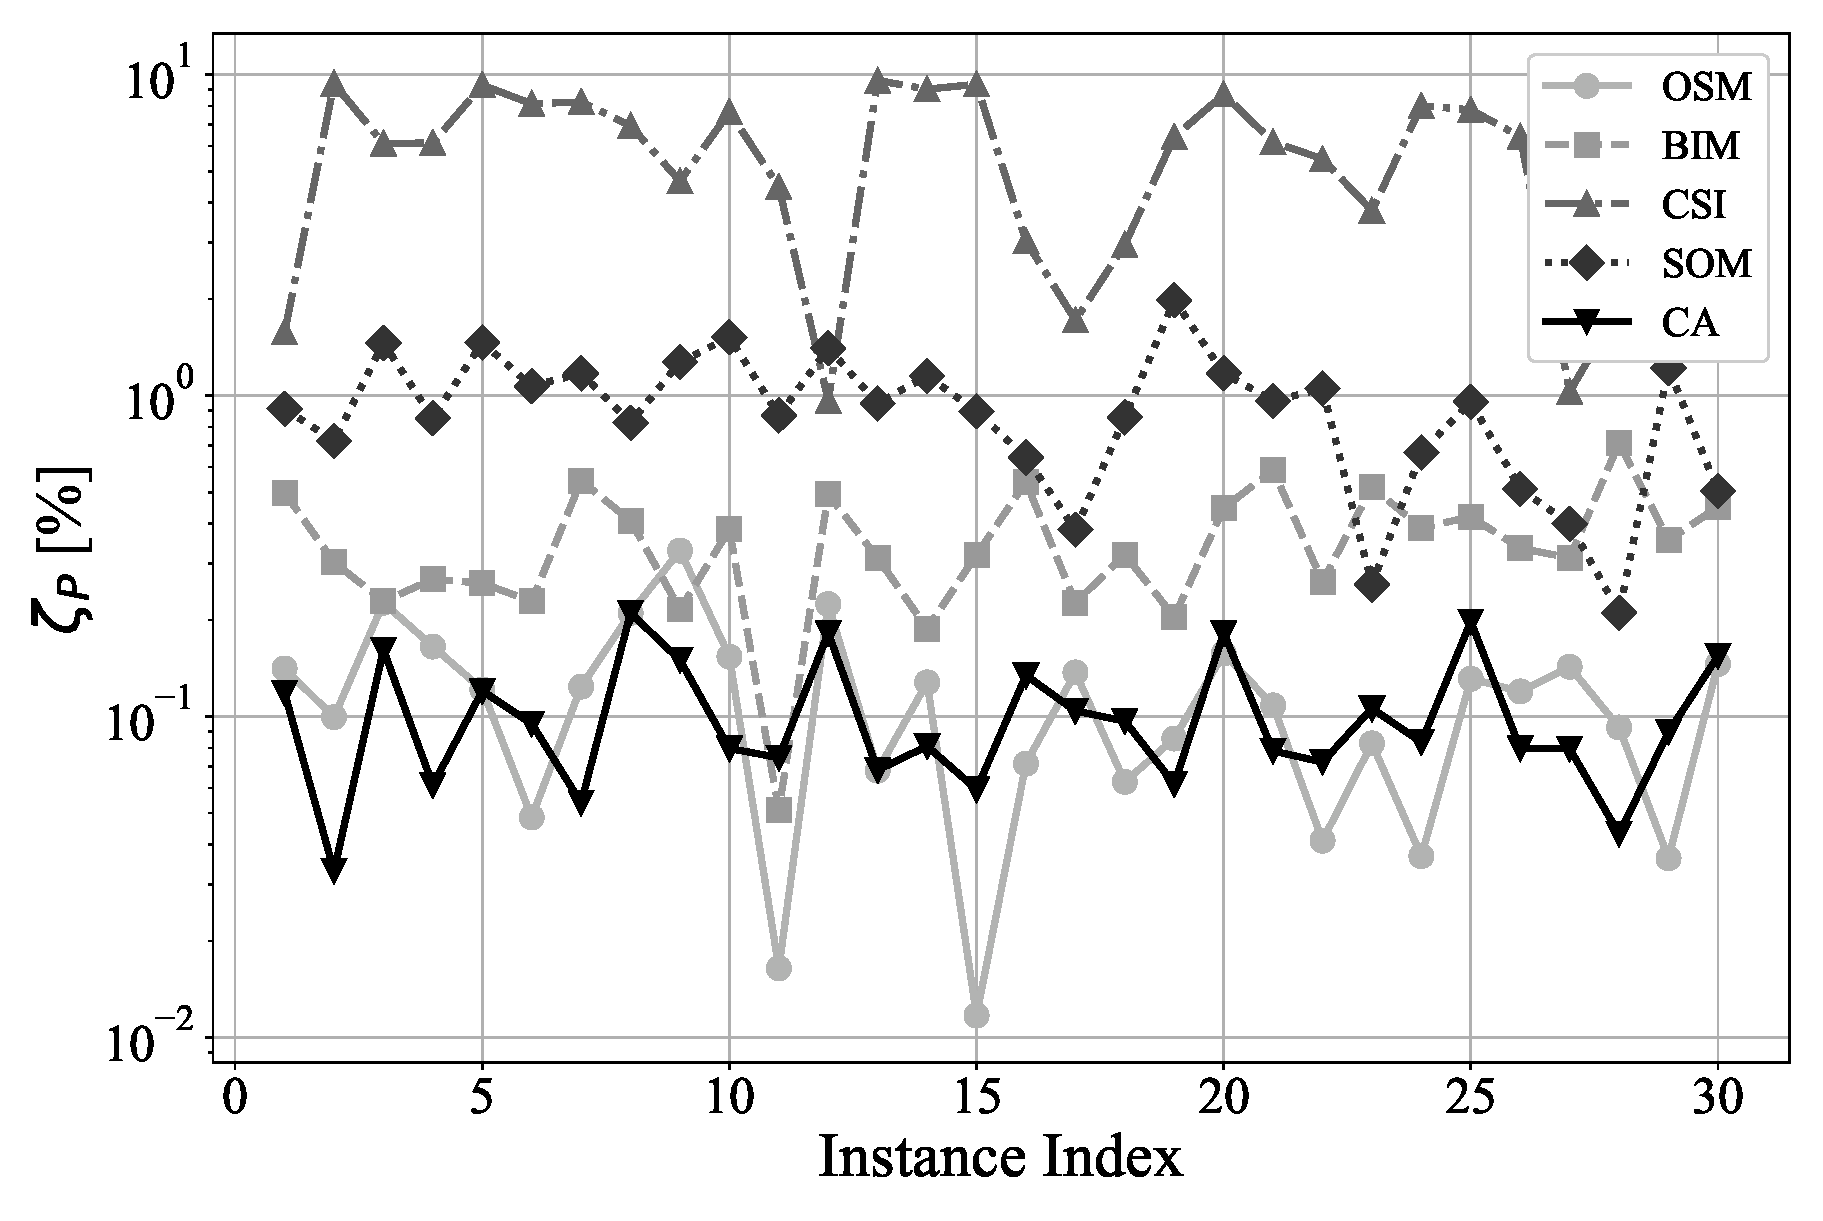
\includegraphics[width=\columnwidth]{./experiments/position/average/figs/plot.eps}\label{fig:position:average:zeta_s}}
                \caption{Position detection study, average performance: (a) Degree of Nonlinearity (DNL) for each scatterer; (b) position error indicator $\zeta_P$ for each algorithm in each instance.}
                \label{fig:position:average}   
            \end{figure}

            While Fig. \ref{fig:position:average:zeta_s} clearly suggests differences in average algorithm performance, RCBD was applied to provide statistical evidence. CSI was excluded from this analysis due to its significantly inferior performance compared to other algorithms. 

            After validating the normality assumption, the RCBD yielded a p-value less than $10^{-30}$, indicating significant differences among algorithms. Multiple paired T-tests with Bonferroni correction revealed p-values less than $10^{-6}$ for all algorithm pairs, except for the OSM-CA comparison. The null hypothesis of equal average performance was rejected for all pairs except OSM-CA, indicating that these two methods demonstrate statistically equivalent performance. The complete p-values are presented in Table \ref{tab:position:average:pvalue}.

            \begin{table*}
                \centering
                \renewcommand{\arraystretch}{1.5}
                \caption{Position detection study, average performance: $p$-values for the paired T-Test with Bonferroni correction.}
                \label{tab:position:average:pvalue}
                \begin{tabular}{ccccccc}
                    Pairs & OSM-BIM & OSM-SOM & OSM-CA & BIM-SOM & BIM-CA & SOM-CA \\\hline
                    $p$-value & $<10^{-9}$ & $<10^{-13}$ & 0.95 & $<10^{-6}$ & $<10^{-10}$ & $<10^{-17}$ \\  
                \end{tabular}
            \end{table*}

            Fig. \ref{fig:position:average:confidence_intervals} shows the 95\% confidence intervals for the mean paired differences of the position error indicator $\zeta_P$ for each algorithm pair. The results demonstrate that OSM and CA achieve superior performance compared to BIM and SOM, while BIM outperforms SOM. However, the mean differences do not exceed 1\% in any case, indicating that although statistically significant differences exist, these differences would only be practically relevant in applications requiring high precision in position detection.

            \begin{figure}
                \centering
                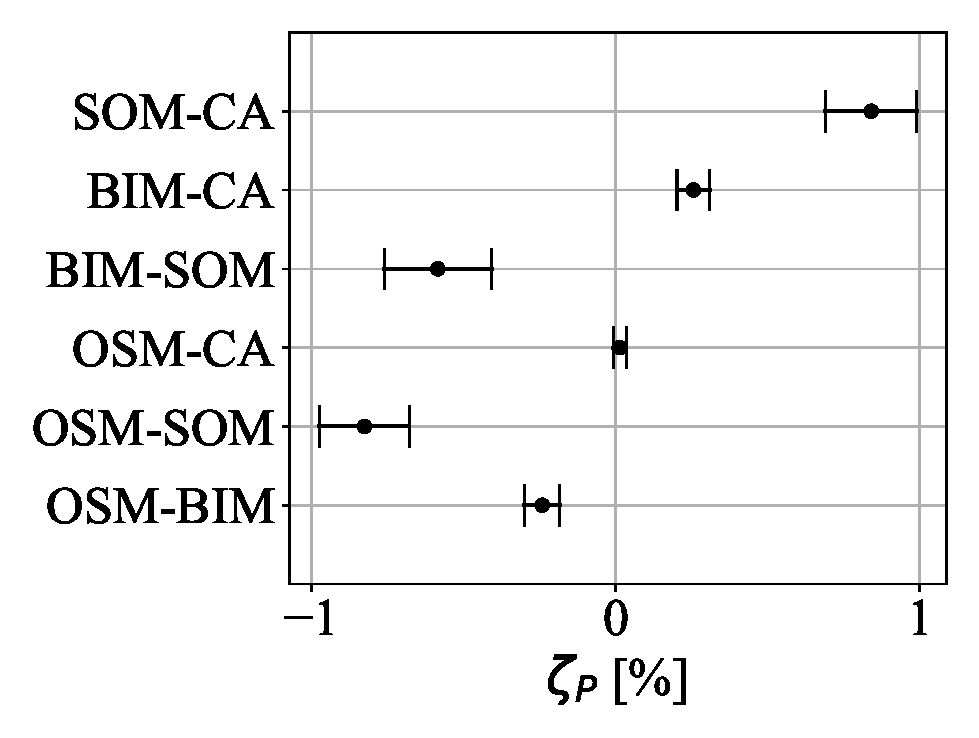
\includegraphics[width=.8\columnwidth]{./experiments/position/average/figs/confidence_intervals.eps}
                \caption{Position detection study, average performance: Confidence intervals (95\%) for the position error indicator $\zeta_P$ for each pair of algorithms.}
                \label{fig:position:average:confidence_intervals}
            \end{figure}

        \subsubsection{Indicator Comparison}\label{sec:results:position:indicatorcomparison}

            Similar to the shape recovery study in Section \ref{sec:results:shape:indicatorcomparison}, an experiment was conducted to compare the proposed position error indicator with commonly used metrics in the literature: RMSE ($\zeta_{\epsilon PAD}$) and SSIM. 

            The experiment employed a star-shaped scatterer with contrast 5 and radius $0.6\lambda_b$, positioned in the upper-right corner as shown in Fig. \ref{fig:position:indicatorcomparison:groundtruth}. The CA algorithm was applied using the same configuration described in Section \ref{sec:results:position:single}. This configuration was chosen because strong scatterers represent a more challenging scenario for algorithms, and CA demonstrates effective position localization capabilities in such scenarios.

            Fig. \ref{fig:position:indicatorcomparison:ca} presents the reconstruction obtained by CA. The contrast was estimated at 5.54 and the circle position is very close to the actual object position. The circle radius was estimated at 0.36$\lambda_b$, significantly smaller. However, this behavior is expected due to differences between the actual geometry and the assumed (circular) geometry in the approximation.

            \begin{figure}
                \centering
                \subfigure[Ground-Truth]{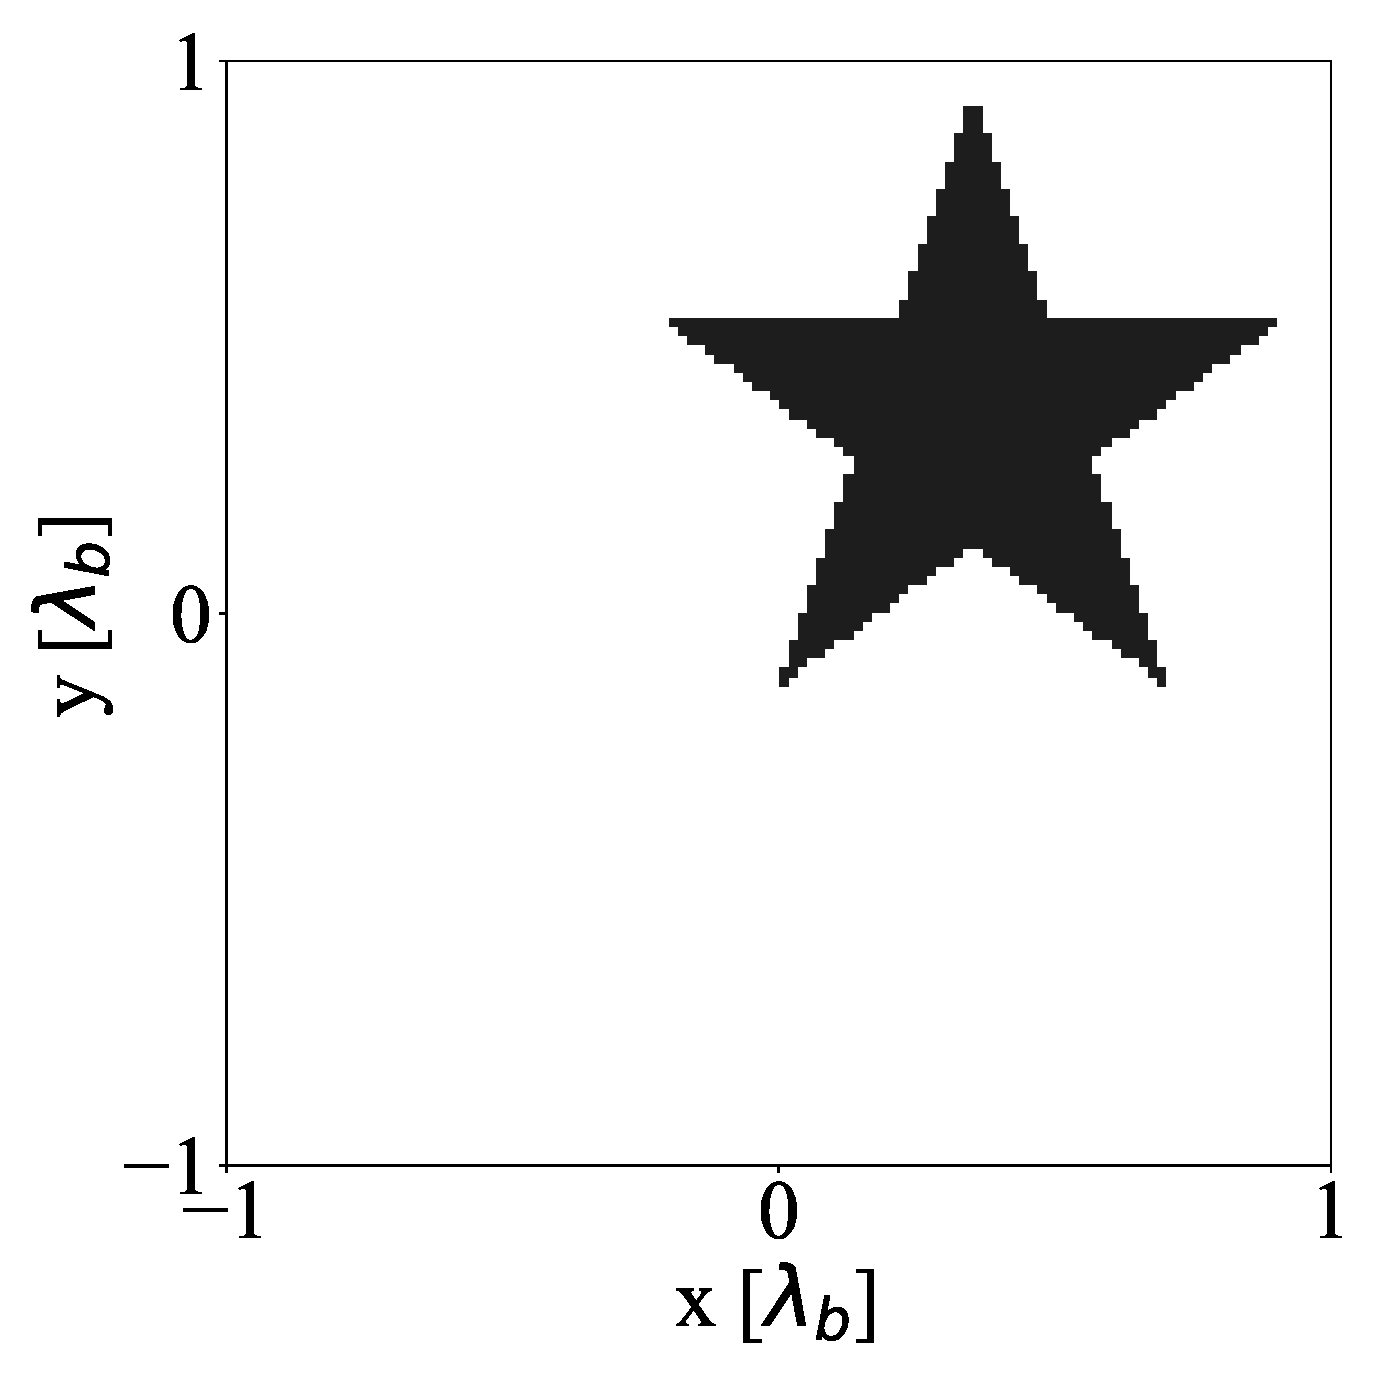
\includegraphics[width=.42\columnwidth]{../experiments/indicatorcomparison/position/figs/groundtruth.eps}\label{fig:position:indicatorcomparison:groundtruth}} \hspace{0.05\columnwidth}
                \subfigure[CA]{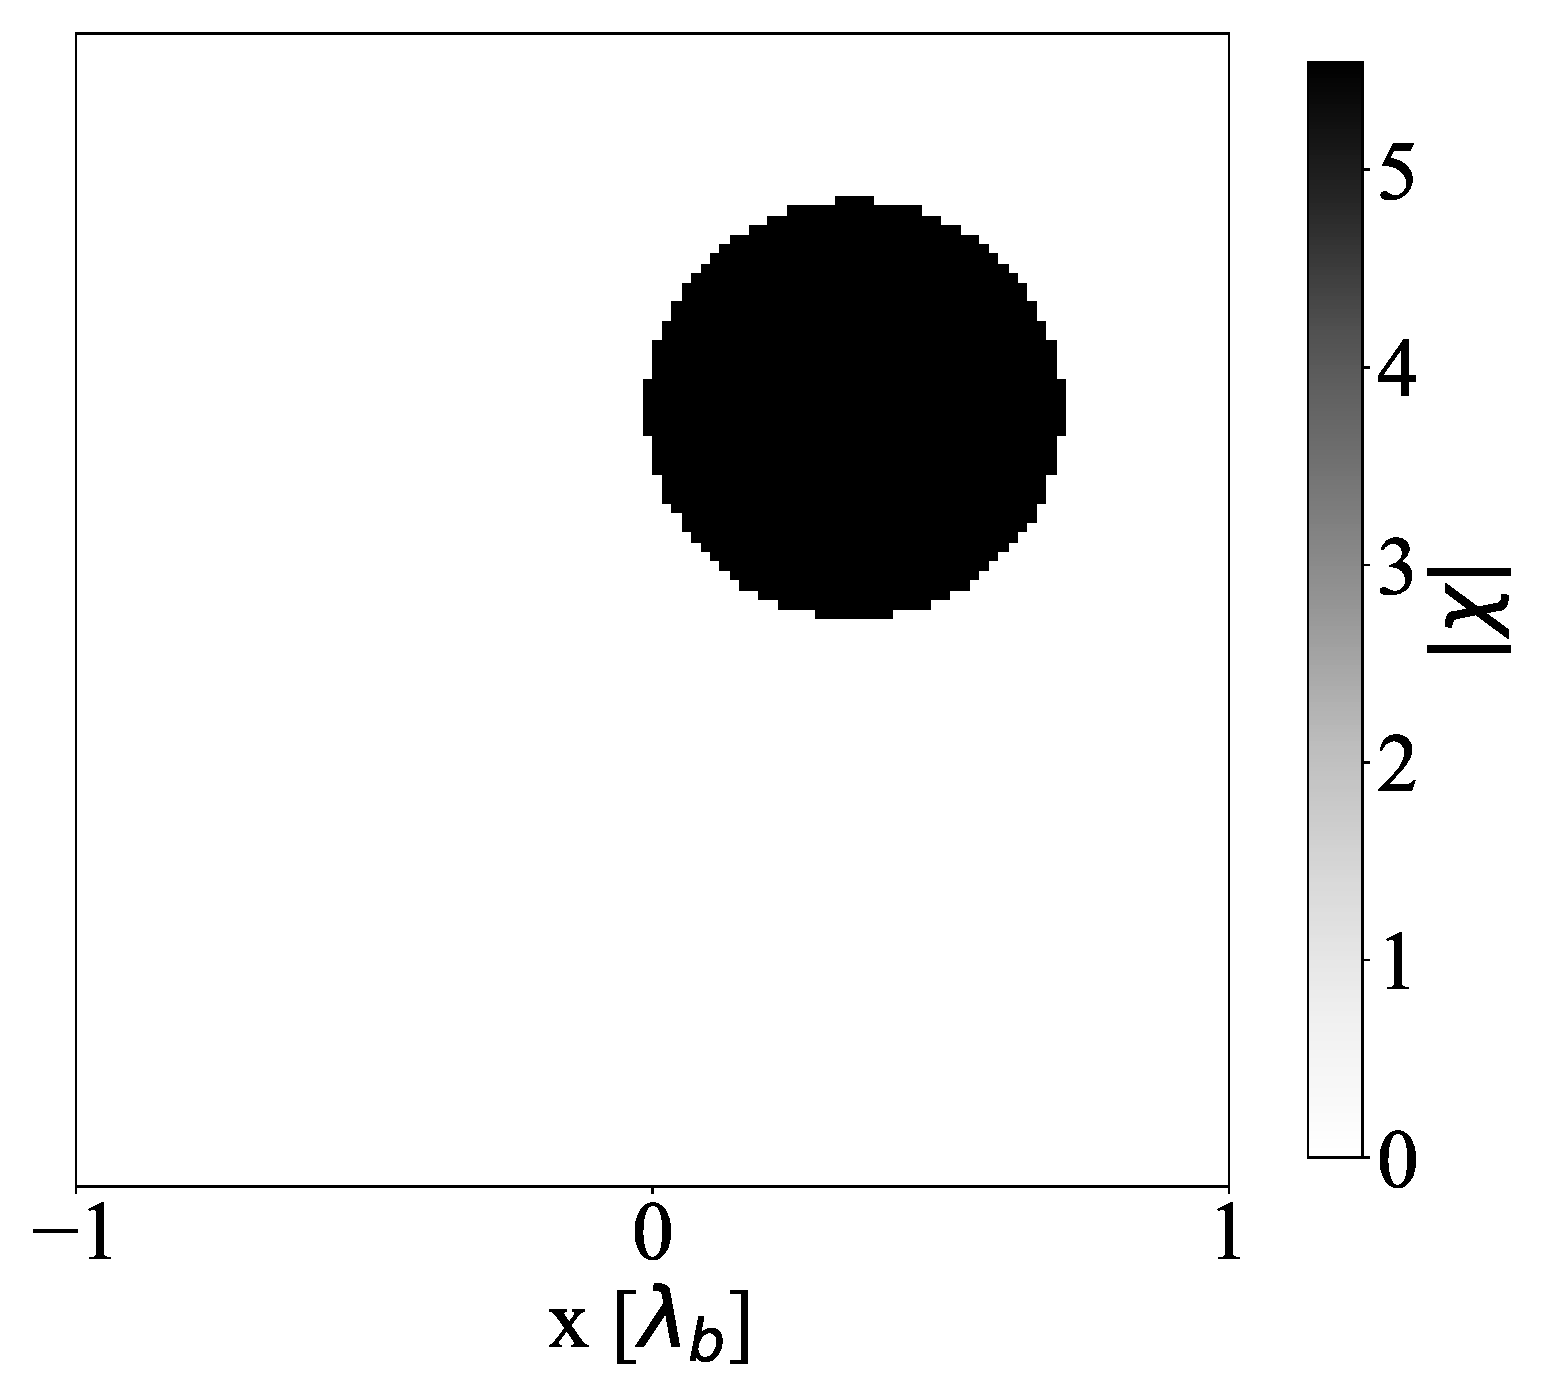
\includegraphics[width=.45\columnwidth]{../experiments/indicatorcomparison/position/figs/ca.eps}\label{fig:position:indicatorcomparison:ca}}
                \caption{Position detection study, indicator comparison: (a) ground-truth and (b) image recovered by CA.}
                \label{fig:position:indicatorcomparison:indicators}
            \end{figure}

            Table \ref{tab:position:indicatorcomparison} summarizes the three indicators for this reconstruction. The $\zeta_P$ indicator achieved a very low value (0.04\%), indicating accurate position detection, as it is suggested by the image recovered. However, both RMSE and SSIM suggest moderate reconstruction quality, with RMSE at 17.13\% and SSIM at 0.8426. This discrepancy occurs because RMSE and SSIM are sensitive to contrast estimation errors and shape approximation, while $\zeta_P$ focuses exclusively on centroid localization, making it more suitable for applications where position accuracy is the primary concern.

            \begin{table}[!htb]
                \centering
                \renewcommand{\arraystretch}{1.5}
                \caption{Position detection study, indicator comparison: position error indicator $\zeta_P$, $\zeta_{\epsilon PAD}$ (RMSE), and SSIM for the image recovered by CA.}
                \label{tab:position:indicatorcomparison}
                \begin{tabular}{ccc}
                    $\zeta_P~(\%)$  & $\zeta_{\epsilon PAD}~(\%/pixel)$ & SSIM \\\hline
                    0.04 & 17.13 & 0.8426 \\
                \end{tabular}   
            \end{table}

    \subsection{Breast Phantom Study}\label{sec:results:breast}

        Finally, a case study using a realistic breast phantom demonstrates the application of the proposed indicators in clinical scenarios. This phantom was obtained from the UWCEM Numerical Breast Phantom Repository \cite{burfeindt2012mri} and corresponds to the Scattered Fibroglandular type (ACR class 2). 

        Since the repository provides three-dimensional phantoms while our scattering model is two-dimensional, a representative cross-section focusing on the breast interior was extracted, as shown in Fig. \ref{fig:breast:recons:ground_truth}. Even though this approach does not capture the complete three-dimensional nature of the breast, it still offers a challenging scenario for evaluating the reconstruction capabilities of the algorithms and it was previously used in related studies \cite{contzano2023fast,wu2024physics,shah2018fast,batista2025eispy2d}. The resulting image contains 328 $\times$ 212 pixels with a spatial resolution of 0.5 mm $\times$ 0.5 mm per pixel. 

        The phantom includes four tissue types: fatty, transitional, fibroconnective/glandular, and skin. The breast is immersed in a homogeneous background medium with relative permittivity $\epsilon_{rb} = 10$ and conductivity $\sigma = 0$ S/m. The operating frequency was set to 1 GHz, with electrical properties (both relative permittivity and conductivity) of breast tissues determined using the Debye model.

        The experimental configuration follows the previous studies: 80 incident sources, 80 measurement points, and 5\% noise level. Under these conditions, the DNL for this experiment is 0.013. Since the interior of the breast is a complex structure, keeping a low DNL value is an important strategy to facilitate the reconstruction. The resolution of the recovered image was set to 80 $\times$ 80 pixels.

        Since fibroglandular tissue represents the region of primary interest within the breast, an adjustment to the indicator calculation methodology was necessary. This modification was required because fatty tissue does not exhibit zero contrast (as it is not homogeneous like the immersion medium). Therefore, object classification based solely on an absolute contrast threshold greater than zero would be inadequate. Consequently, the threshold for object classification in the original image was set as 70\% of the value between the maximum and minimum contrast values. Through this approach, the fibroglandular tissue region was effectively isolated, allowing for relevant shape and position error calculations.

        It is important to emphasize that the proposed indicators are designed as physics-based quantitative metrics for evaluating algorithmic performance in image reconstruction, rather than as clinical diagnostic tools. They are intended to facilitate algorithm development, benchmarking studies, and performance assessment in controlled scenarios where ground truth is known. While the indicators show promise for various applications including medical imaging, their correlation with clinical expert assessments in real-world medical scenarios remains a subject for future investigation.

        The algorithm parameters were readjusted as follows:
        \begin{itemize}
            \item Linear Sampling Method (LSM):
            \begin{itemize}
                \item Threshold: 0.95;
                \item Regularization Method: Tikhonov with $\alpha = 1$.
            \end{itemize}
            \item Orthogonality Sampling Method (OSM):
            \begin{itemize}
                \item Threshold: 0.9;
            \end{itemize}
            \item Born Iterative Method (BIM):
            \begin{itemize}
                \item Regularization Method: Tikhonov with $\alpha = 10$
                \item Stopping Criterion: 10 iterations.
            \end{itemize}
            \item Contrast Source Inversion (CSI):
            \begin{itemize}
                \item Stopping Criterion: 1500 iterations.
            \end{itemize}
            \item Subspace Optimization Method (SOM):
            \begin{itemize}
                \item Stopping Criterion: 100 iterations.
                \item Eigenvalue Cutoff Index: 15.
            \end{itemize}
        \end{itemize}

        Fig. \ref{fig:breast:recons} presents the reconstruction results obtained by each algorithm. All methods successfully detected the fibroglandular tissue region, although the quantitative algorithms varied in their contrast estimations. CSI and SOM underestimated the contrast values, while BIM had the closest estimation. As expected, the algorithms struggled to reconstruct the thin skin layer. However, the boundary between the fatty tissue and the immersion medium is observable in several reconstructions.

        \begin{figure*}[!htb]
            \centering
            \subfigure[Ground-Truth]{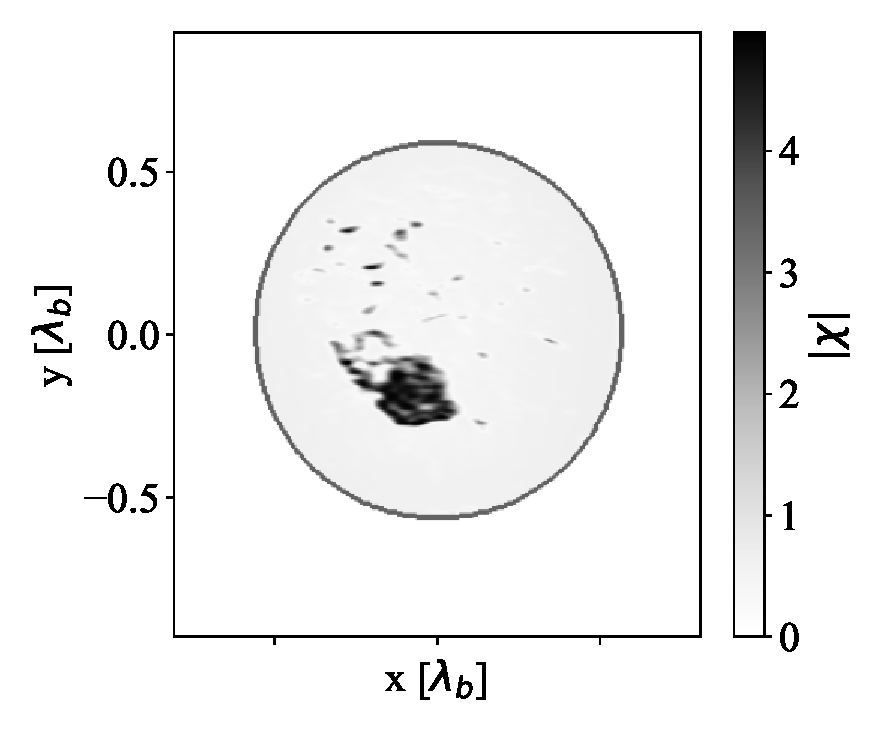
\includegraphics[height=0.55\columnwidth]{../experiments/breast/figs/0.eps}\label{fig:breast:recons:ground_truth}}
            \subfigure[LSM]{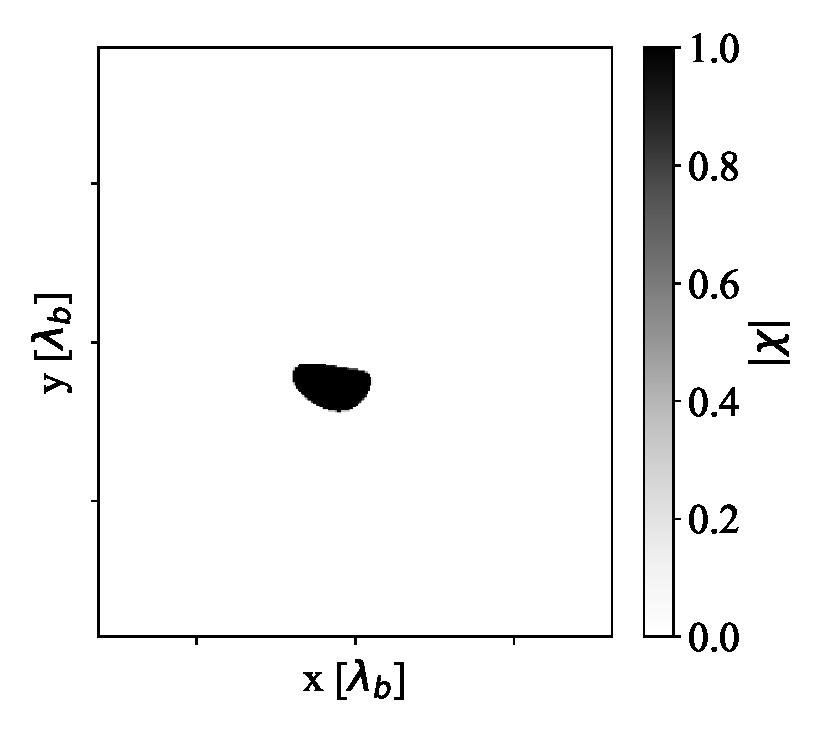
\includegraphics[height=0.55\columnwidth]{../experiments/breast/figs/1.eps}}
            \subfigure[OSM]{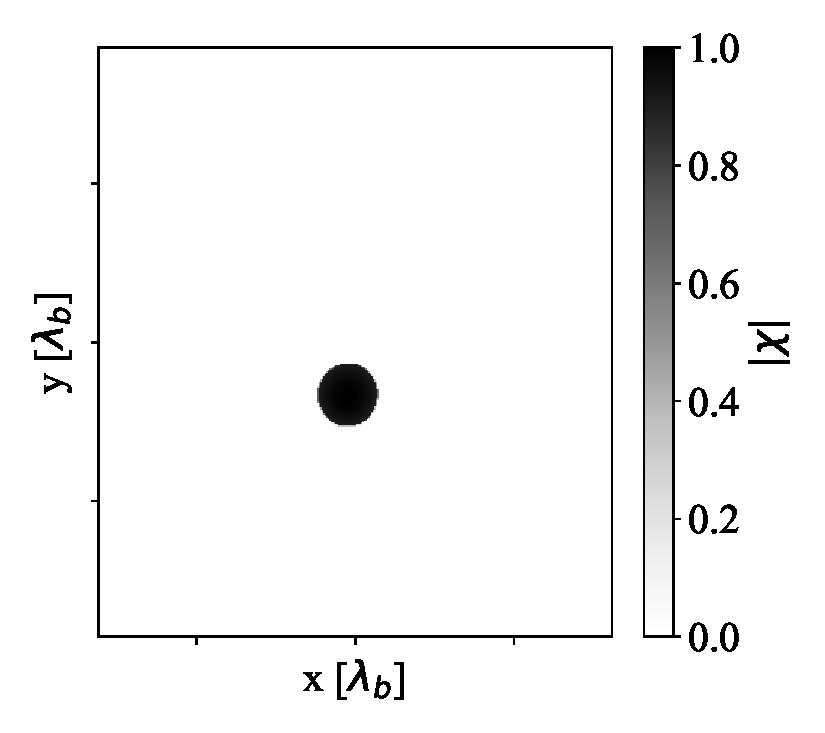
\includegraphics[height=0.55\columnwidth]{../experiments/breast/figs/2.eps}} \\
            \subfigure[BIM]{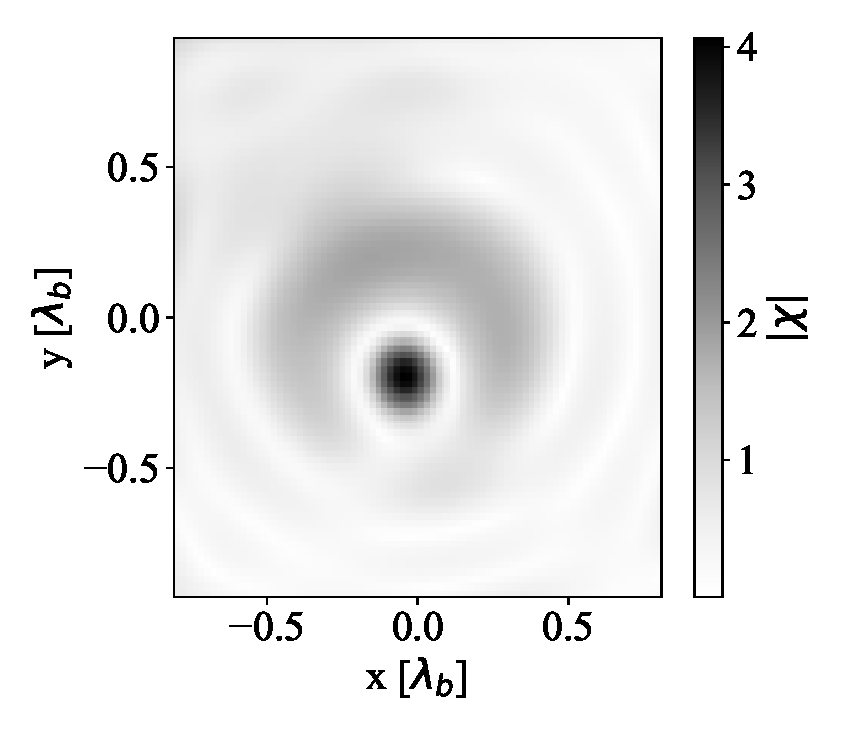
\includegraphics[height=0.55\columnwidth]{../experiments/breast/figs/3.eps}} 
            \subfigure[CSI]{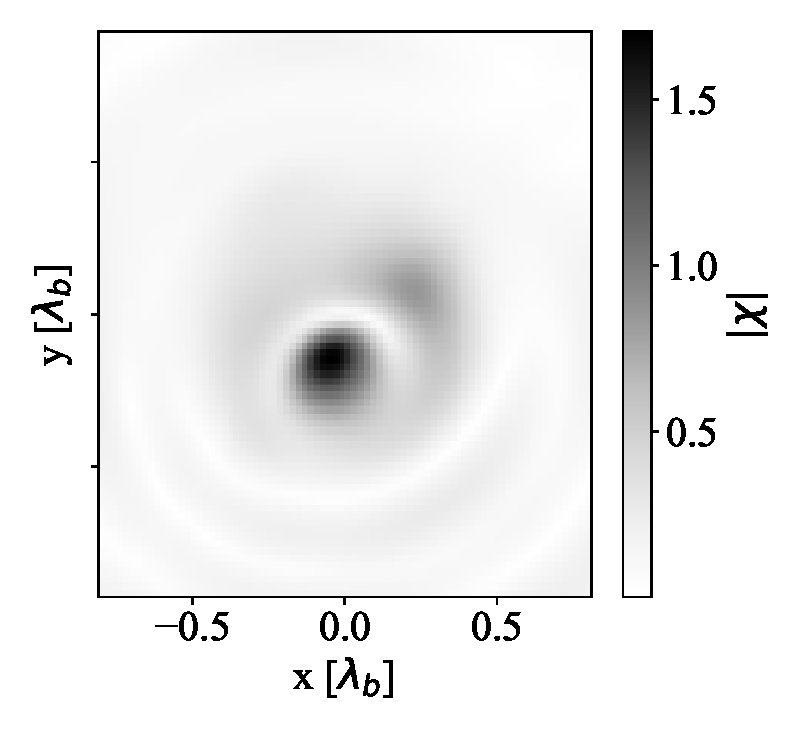
\includegraphics[height=0.55\columnwidth]{../experiments/breast/figs/4.eps}}
            \subfigure[SOM]{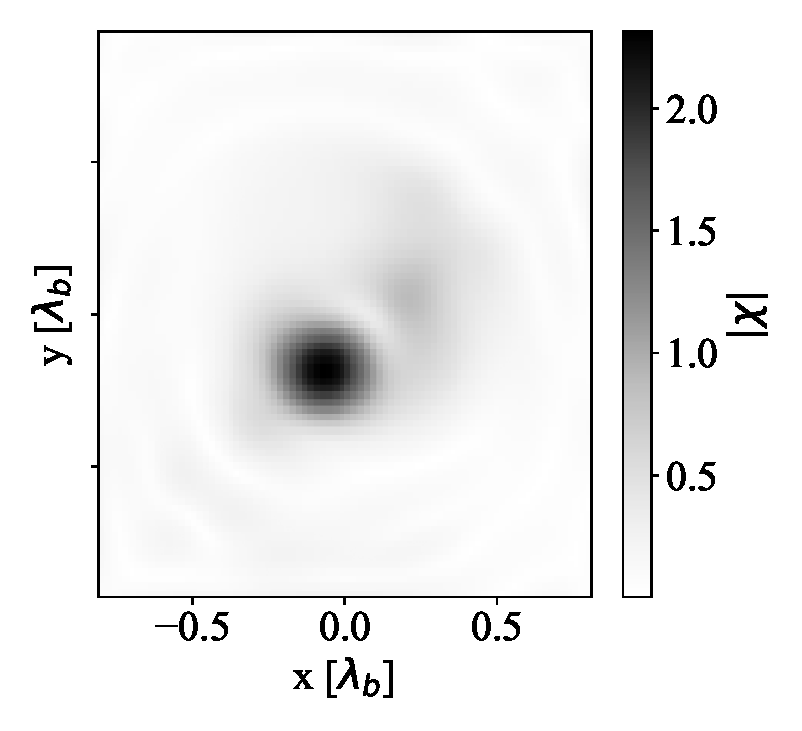
\includegraphics[height=0.55\columnwidth]{../experiments/breast/figs/5.eps}}
            % \subfigure[CA]{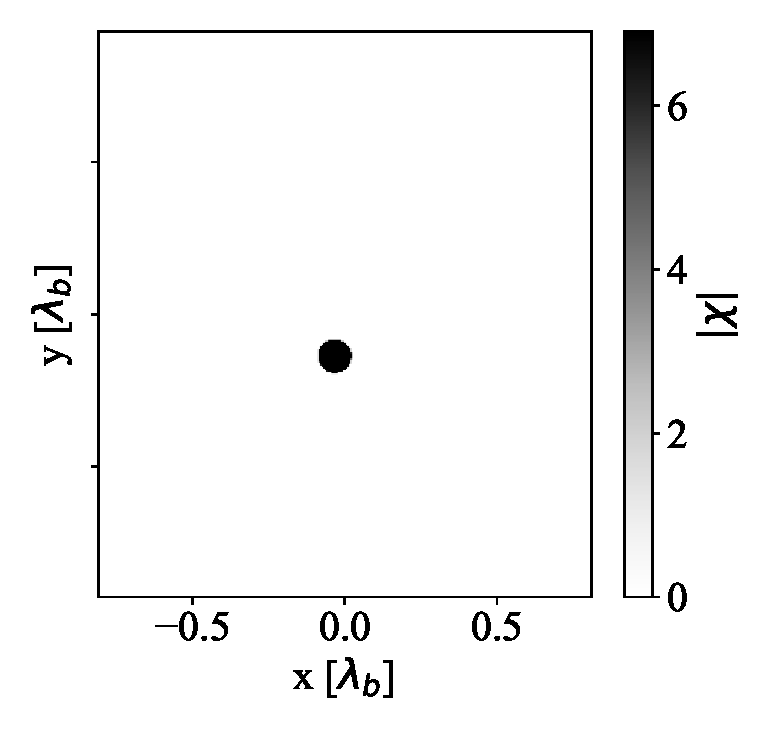
\includegraphics[height=0.4\columnwidth]{../experiments/breast/figs/6.eps}}
            \caption{Breast phantom study: ground-truth and reconstructed images by each algorithm.}
            \label{fig:breast:recons}
        \end{figure*}

        Table \ref{tab:breast:indicators} presents the shape and position error indicators for each algorithm. The shape error values exceed 57\% for all methods, indicating significant challenges in accurately reconstructing the glandular tissue structure. Since this tissue size is small compared to the image dimensions, variations in the size and shape of the tissue reconstruction can significantly impact the shape indicator. Regarding position detection, all algorithms achieved relatively low position errors (below 5\%), with SOM demonstrating the best performance at 1.6\%.

        \begin{table}[!htb]
            \centering
            \renewcommand{\arraystretch}{1.5}
            \caption{Breast phantom study: shape and position error indicators for each algorithm.}
            \label{tab:breast:indicators}
            \begin{tabular}{cccccc}
                Method & LSM & OSM & BIM & CSI & SOM \\\hline %  & CA \\\hline
                $\zeta_S$ (\%) & 83.6 & 78.6 & 57.2 & 81.4 & 118.8 \\ % & 86.5 \\
                $\zeta_P$ (\%) & 2.2 & 4.3 & 3.1 & 3.5 & 1.6 %% & 4.2 \\
            \end{tabular}   
        \end{table}

\section{Conclusion}\label{sec:conclusion}

    Since many algorithms have been and continue to be proposed for the electromagnetic inverse scattering problem, and it is important to have indicators capable of measuring algorithm performance across different aspects, this work aimed to develop two novel indicators that can measure two relevant problem aspects in a more isolated manner: scatterer localization and geometry. These shape and position error indicators were developed using thresholding and contour detection tools to reduce the impact of contrast estimation precision, enabling more independent measurement of these aspects. Although the calculation of these indicators depends on threshold level selection, they enable adequate comparisons between qualitative and quantitative algorithms, particularly in single scatterer scenarios. Therefore, through standardized test sets, these indicators can serve as significant tools for evaluating and comparing the performance of methods proposed in the literature.

    It is also worth highlighting that, based on the proposed indicators, the computational experiments conducted through benchmarking studies were able to provide stronger conclusions about the performance of traditional algorithms in the literature when they are compared. The studies demonstrated that: (a) in scenarios with a single scatterer and low DNL, BIM achieves the best average performance in scatterer shape recovery compared to other considered algorithms; (b) in scenarios involving small, high-contrast scatterers, OSM and CA achieve the best average performance in scatterer localization. Moreover, experiments comparing the proposed indicators with commonly used metrics in the literature revealed that the new indicators are less sensitive to background medium variations and contrast estimation errors, making them more suitable for applications where shape and position accuracy are the primary concerns. Additional studies could be conducted to explore algorithm performance differences more thoroughly, though this was not the primary objective of this work.

    Future investigations may be undertaken to enhance the proposed indicators. One possibility would be to compare scatterer geometries through object vertices, which would require robust detection of corresponding objects (in multiple scatterer cases) between real and reconstructed images, and the handling of differences in contour point quantities. This could enable the creation of an indicator to measure geometry quality without considering scatterer size reconstruction precision. Others indicators can be explored as well, such as CNR (Contrast-to-Noise Ratio), Dice, IoU (Intersection over Union), Hausdorff Distance, among others. Another possible direction would be developing different test sets that explore various problem scenarios to serve as standards for algorithm comparison. Finally, adapting the indicators for three-dimensional problems represents another viable path for future research.

\appendices

\section*{Acknowledgment}
The authors would like to thank Lucas S. Batista for his guidance and manuscript review. They also thank the reviewers for their valuable comments and suggestions that helped improve the quality of this work.

\bibliographystyle{IEEEtran}
\bibliography{IEEEabrv,mybib.bib}

\begin{IEEEbiography}[{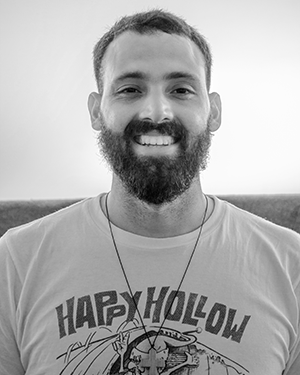
\includegraphics[width=1in,height=1.25in,clip,keepaspectratio]{./figs/batan.png}}]
    {André Costa Batista} was born in Ipatinga, MG, Brazil in 1994. He received the B.S. degree in Systems Engineering from the Universidade Federal de Minas Gerais (UFMG), in 2019. He received the Ph.D. degree in Electrical Engineering from the same university in 2023. His is currently an Assistant Professor with the Department of Electrical Engineering, UFMG, since 2024.
    
    His research interest includes microwave imaging, inverse problems. computational electromagnetism, optimization (linear, combinatorial, non-linear, multi-criteria), evolutionary computation, and systems engineering.
\end{IEEEbiography}

\begin{IEEEbiography}[{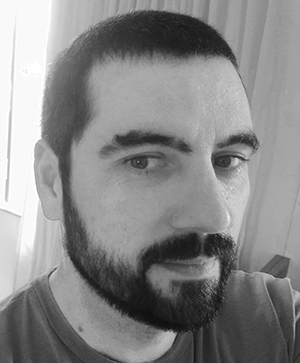
\includegraphics[width=1in,height=1.25in,clip,keepaspectratio]{./figs/adria.png}}]
    {Ricardo Adriano} was born in Belo Horizonte, Brazil in 1979. He received the bachelor's and Ph.D. degrees in electrical engineering from the Universidade Federal de Minas Gerais (UFMG), Belo Horizonte, Brazil, in 2003 and 2007, respectively.
	
	He is currently an Associate Professor with the Department of Electrical Engineering, UFMG. He has been directly involved with UFMG's undergraduate courses on Systems Engineering and Aerospace Engineering, and with the graduate course on Electrical Engineering. His current research involves computational electromagnetics as well as electro-magnetic compatibility and optimization of electromagnetic devices.
\end{IEEEbiography}

\EOD

\end{document}
